% ============================================================
% 数学建模竞赛 LaTeX 国赛通用模板，严格参考，可微微创新
% 参考当前论文主稿的版式结构，并抽象为可复用模板
% 编译方式：XeLaTeX
% ============================================================
\documentclass[12pt,a4paper]{article}

% ---------- 中文支持 ----------
\usepackage{ctex}
\setCJKmainfont{SimSun}
\setCJKsansfont{SimHei}
\setmainfont{Times New Roman}
\usepackage{unicode-math}
\setmathfont{Cambria Math}

% ---------- 页面与行距 ----------
\usepackage[top=2.5cm, bottom=2.5cm, left=2.0cm, right=2.0cm]{geometry}
\usepackage{setspace}
\onehalfspacing
\setlength{\parindent}{2em}

% ---------- 页眉页脚 ----------
\usepackage{fancyhdr}
\usepackage{appendix}
\pagestyle{fancy}
\fancyhf{}
\setlength{\headheight}{14pt}
\fancyfoot[C]{{\fontsize{9pt}{11pt}\selectfont\rmfamily \thepage}}
\renewcommand{\headrulewidth}{0pt}

% ---------- 数学与符号 ----------
\usepackage{amsmath,amsthm}
\usepackage{bm}
\usepackage{mathrsfs}

% ---------- 图表 ----------
\usepackage{graphicx}
\graphicspath{{./}{./figures/}{./images/}}
\usepackage{subcaption}
\usepackage{float}
\usepackage[table,xcdraw]{xcolor}
\usepackage{booktabs}
\usepackage{longtable}
\usepackage{array}
\usepackage{multirow}

% ---------- 算法 ----------
\usepackage{algorithm}
\usepackage{algpseudocode}
\renewcommand{\algorithmicrequire}{\textbf{Input:}}
\renewcommand{\algorithmicensure}{\textbf{Output:}}

% ---------- 引用与链接 ----------
\usepackage{hyperref}
\hypersetup{colorlinks=true,linkcolor=black,citecolor=black}

% ---------- 代码环境 ----------
\usepackage{listings}
\lstset{
    basicstyle=\footnotesize\ttfamily,
    numbers=left,
    numberstyle=\tiny,
    frame=single,
    breaklines=true,
    language=Python
}

% ---------- 其他 ----------
\usepackage{indentfirst}
\usepackage{enumitem}
\usepackage{makecell}
\usepackage{pifont}
\usepackage{titlesec}

% ---------- 字体与标题样式 ----------
\newcommand{\titlefont}{\fontsize{16pt}{20pt}\selectfont\heiti\bfseries}
\newcommand{\sectiontitlefont}{\fontsize{14pt}{18pt}\selectfont\heiti\bfseries}
\newcommand{\levelonefont}{\fontsize{14pt}{18pt}\selectfont\heiti\bfseries}
\newcommand{\leveltwofont}{\fontsize{12pt}{16pt}\selectfont\heiti\bfseries}
\newcommand{\levelthreefont}{\fontsize{12pt}{16pt}\selectfont\heiti}
\newcommand{\bodyfont}{\fontsize{12pt}{16pt}\selectfont\songti}
\newcommand{\keywordfont}{\fontsize{12pt}{16pt}\selectfont\heiti\bfseries}
\newcommand{\paperstrong}[1]{{\heiti #1}}
\newcommand{\appendixtitlefont}{\fontsize{14pt}{18pt}\selectfont\heiti\bfseries}
\newcommand{\stepfont}[1]{{\fontsize{12pt}{16pt}\selectfont\fontspec{Times New Roman}\bfseries Step~#1}}
\newcommand{\bibfont}{\fontsize{10.6pt}{15pt}\selectfont}
\newcommand{\supercite}[1]{\textsuperscript{\cite{#1}}}

\renewcommand{\thesection}{{\heiti\chinese{section}}}
\renewcommand{\thesubsection}{\arabic{section}.\arabic{subsection}}
\renewcommand{\thesubsubsection}{\arabic{section}.\arabic{subsection}.\arabic{subsubsection}}
\titleformat{\section}{\centering\levelonefont}{\thesection、}{0.6em}{}
\titleformat{\subsection}{\leveltwofont}{\thesubsection}{0.6em}{}
\titleformat{\subsubsection}{\levelthreefont}{\thesubsubsection}{0.6em}{}

% ============================================================
\begin{document}
\label{body:start}

% ---------- 第一页：标题与摘要 ----------
\begin{center}
\vspace*{0.6cm}
{\titlefont 锂离子电池快充策略对寿命衰减的影响建模与优化\par}
\vspace{0.4cm}
\end{center}

\begin{center}
{\sectiontitlefont 摘要}
\end{center}

\vspace{0.3cm}
\bodyfont

\indent 锂离子电池的快充效率直接决定用户体验与系统运行效率，而较高的充电电流会加剧极化、热效应与副反应，导致容量衰减加快。本文基于 MIT-Stanford 公开的 49 块 A123 18650 磷酸铁锂快充循环老化数据集，围绕"数据整理—策略影响—寿命预测—策略优化"四层递进主线，建立稳健数据清洗、可解释寿命基线、多维增强轨迹预测与双层策略优化的完整建模链路，为快充策略工程化设计提供量化依据。

\indent \paperstrong{针对问题一}，本文对 49 块电池逐电池执行 Hampel/MAD 异常检测（$\sigma=5.0$）与 Savitzky-Golay 滤波（$w=11$）完成 Capacity 清洗，并严格将 1$\sim$150 圈与 151$\sim$200 圈分段处理以防信息泄漏。在\paperstrong{嵌套 LOBO}验证下，\paperstrong{单调幂律}模型 $\mathrm{SOH}(n)=a-bn^c$（$n_0=21$）外层 RMSE 为\paperstrong{$0.048\%$}，39/40 折选择幂律，EOL 一致性中位差仅 $0.20$，为后续分析提供稳健寿命基线。

\indent \paperstrong{针对问题二}，本文以 9 种策略执行 Kruskal-Wallis 检验，给出\paperstrong{$H=24.6$，$p=0.00038$}。为解除 $C_1,Q_1,C_2$ 耦合，将三参数重表示为总体倍率水平 $A$ 与倍率分配差 $D$，VIF 由 $12.4$ 降至\paperstrong{$1.8$}；参数 $A$ 与 IR 斜率 Spearman 相关系数达\paperstrong{$0.928$}，经分层 Bootstrap 与精确置换检验验证。

\indent \paperstrong{针对问题三}，本文建立\paperstrong{Trend-PCA-Ridge}增强模型：个体近期趋势承担主预测，PCA 压缩 50 维残差轨迹，Ridge 利用早期健康特征预测个体修正。嵌套 LOBO 加一标准误规则下，100 圈窗口取得\paperstrong{OOF MAE $=0.080\%$}，9 块测试电池 EOL 中位误差仅 $0.73$ 圈，IR 状态一致性达\paperstrong{$98.74\%$}。

\indent \paperstrong{针对问题四}，本文构建\paperstrong{双层策略优化架构}：A 层基于 9 种已有策略在 49 块电池前 150 圈的真实充电时间与稳定退化率经验 Pareto，B 层以问题二冻结的参数位置为锚，在 $9.9900\sim10.0132$ min 局部可行域做 Sobol 候选生成与 $\mathrm{Q}_{90}(r)$ 鲁棒优化，再以问题三未来 50 圈轨迹做一致性审计。推荐\paperstrong{A级主方案 $5\_3C\_54PER\_4C$}（实测时间 $10.0429$ min，$r_\text{stable}=2.053\times10^{-5}$/圈）与\paperstrong{B 级工程候选 $5.05C$-$50$-$4.42C$}（$P(\Delta<0)=1.0$）。

\indent 综上，本文以"稳健清洗—可解释基线—多维增强—双层优化"为递进主线，四问共享同一数据口径与平滑曲线，形成层次分明、逻辑闭合的建模体系，为快充策略工程化设计与寿命预测提供可追溯、可复现的量化依据。

\indent {\keywordfont \paperstrong{关键词：}} \paperstrong{锂离子电池}；\paperstrong{快充策略优化}；\paperstrong{Pareto 非支配}；\paperstrong{鲁棒优化}；\paperstrong{Trend-PCA-Ridge}；\paperstrong{单调幂律退化}\label{abstract:end}

\newpage

% ============================================================
\section{问题重述}
% ============================================================

\subsection{问题背景}

锂离子电池是新能源汽车、储能电站与便携电子设备的核心能量载体，其充电速度与循环寿命之间的矛盾长期制约快充策略的工程化设计。磷酸铁锂电池因安全性高、循环寿命长而被广泛采用，但在高倍率充电条件下，锂离子在负极界面处的扩散与嵌入速率难以匹配外部电流，进而引发浓差极化、欧姆热、析锂与电解液氧化等副反应，导致活性锂损失与界面阻抗增长，宏观上表现为可用容量不可逆衰减\supercite{ref12,ref13}。如何在保证充电时间满足用户体验的前提下，合理分配不同荷电状态区间的充电电流，使寿命衰减尽量平缓，是快充策略优化的核心科学问题。

本赛题采用 Attia 等人在 Nature Energy 公开的 MIT-Stanford 快充循环老化数据集\supercite{ref8}。该数据集包含 49 块 A123 APR18650M1A 磷酸铁锂电池，额定容量 $1.1$ Ah，标称电压 $3.3$ V，在 $30^\circ$C 恒温箱中以 72 种不同快充策略循环至失效或截止圈数。每块电池在每圈记录放电容量、内阻（IR）、平均与最大表面温度、充电时间等状态变量，循环终止条件为额定容量衰减至 $80\%$ 即 end-of-life（EOL）。不同策略在第一阶段恒流充电电流 $C_1$、第一阶段截止荷电状态 $Q_1$、第二阶段恒流充电电流 $C_2$ 上存在差异，$Q_1$ 至 $80\%$ SOC 之间由 $C_2$ 完成，其后转入恒压阶段至充满。

数据集的设计动机在于：通过在 0$\sim$80\% SOC 窗口内分配不同的电流组合，量化各策略对寿命衰减的影响，进而搜索兼顾充电时间与寿命的最优策略。本赛题在该数据集基础上提出四个递进的子问题，要求参赛者完成数据清洗、策略影响统计推断、寿命预测与策略优化。

\subsection{问题提出}

\textbf{问题一}要求对 49 块电池的循环数据进行清洗与稳健性处理，去除异常点并提取可用于后续建模的健康状态曲线，再建立能够刻画容量衰减规律的基准寿命模型，给出各策略在统一口径下的寿命估计，为后续统计推断与预测提供可比的退化指标。

\textbf{问题二}要求在问题一清洗结果基础上，量化不同快充策略对寿命衰减的统计影响，识别影响寿命的关键充电参数与荷电状态区间，并通过合理的参数化方式构建可解释的参数效应模型，为策略优化提供机理层面的依据。

\textbf{问题三}要求仅利用每块电池早期的循环数据，预测其未来 SOH 轨迹与最终寿命，并对预测结果进行交叉验证与不确定性评估，为远期外推提供跨状态变量的间接支持，检验模型在工程落地中的可推广性。

\textbf{问题四}要求在兼顾快充时间与寿命衰减两个目标的前提下，搜索更优的快充策略。本问需要在问题二建立的参数效应模型与问题三的轨迹预测能力之上，设计可工程实现的多目标优化框架，给出明确的推荐策略及其稳健性证据，并对推荐结果进行压力测试与一致性审计。

% ============================================================
\section{问题分析}
% ============================================================

四个子问题构成"数据整理—策略影响—寿命预测—策略优化"的递进主线，前问的结果作为后问的输入与约束，形成逻辑闭合的建模链路。

问题一的核心难点在于数据噪声与寿命外推的双重不确定性。原始数据中存在由传感器抖动、热失控早期事件与设备重启引入的孤立尖峰，若直接拟合会扭曲退化斜率；同时，EOL 判定依赖对 80\% 容量阈值的反向插值，不同模型结构对短窗口数据的拟合优度可能高估外推稳定性。因此，本问需要稳健的异常检测、分段处理防止信息泄漏，以及嵌套留一法验证以同时控制模型选择偏差与外推误差。

问题二的难点在于策略参数的强耦合与样本量有限。$C_1,Q_1,C_2$ 三者通过充电时间公式相互约束，直接回归会因共线性导致系数不可解释；9 种完整策略样本量偏小，常规方差分析假设难以满足。因此本问需要非参数检验处理分布自由性，并通过基于充电时间公式的重参数化解除耦合，再结合 Bootstrap 与置换检验控制小样本下的推断风险。

问题三的难点在于早期窗口信息量有限与跨电池异质性。仅用前若干圈数据预测百圈后的 SOH，要求模型既能捕捉个体退化趋势，又能借助群体先验补偿早期数据不足；同时不同电池的退化斜率、温度响应与内阻演化存在显著差异，单一模型难以兼顾。因此本问需要多尺度特征工程、降维与正则化回归的组合，以及嵌套验证控制模型复杂度。

问题四的难点在于多目标、多约束与跨问模型继承。快充时间与寿命衰减构成天然冲突，而充电时间约束带由 6 个真实策略的理论时间构成，可行域为局部窄带；同时问题二冻结的参数效应模型仅由 6 个 NEWSTRUCTURE 策略标定，外推风险需由 Bootstrap 与 LOPO 压力测试控制，问题三的轨迹预测需作为一致性审计约束。因此本问需要双层架构：经验 Pareto 提供全局参照，局部鲁棒优化在窄带内搜索，问题三对未来轨迹做反向校验。

\begin{figure}[H]
\centering
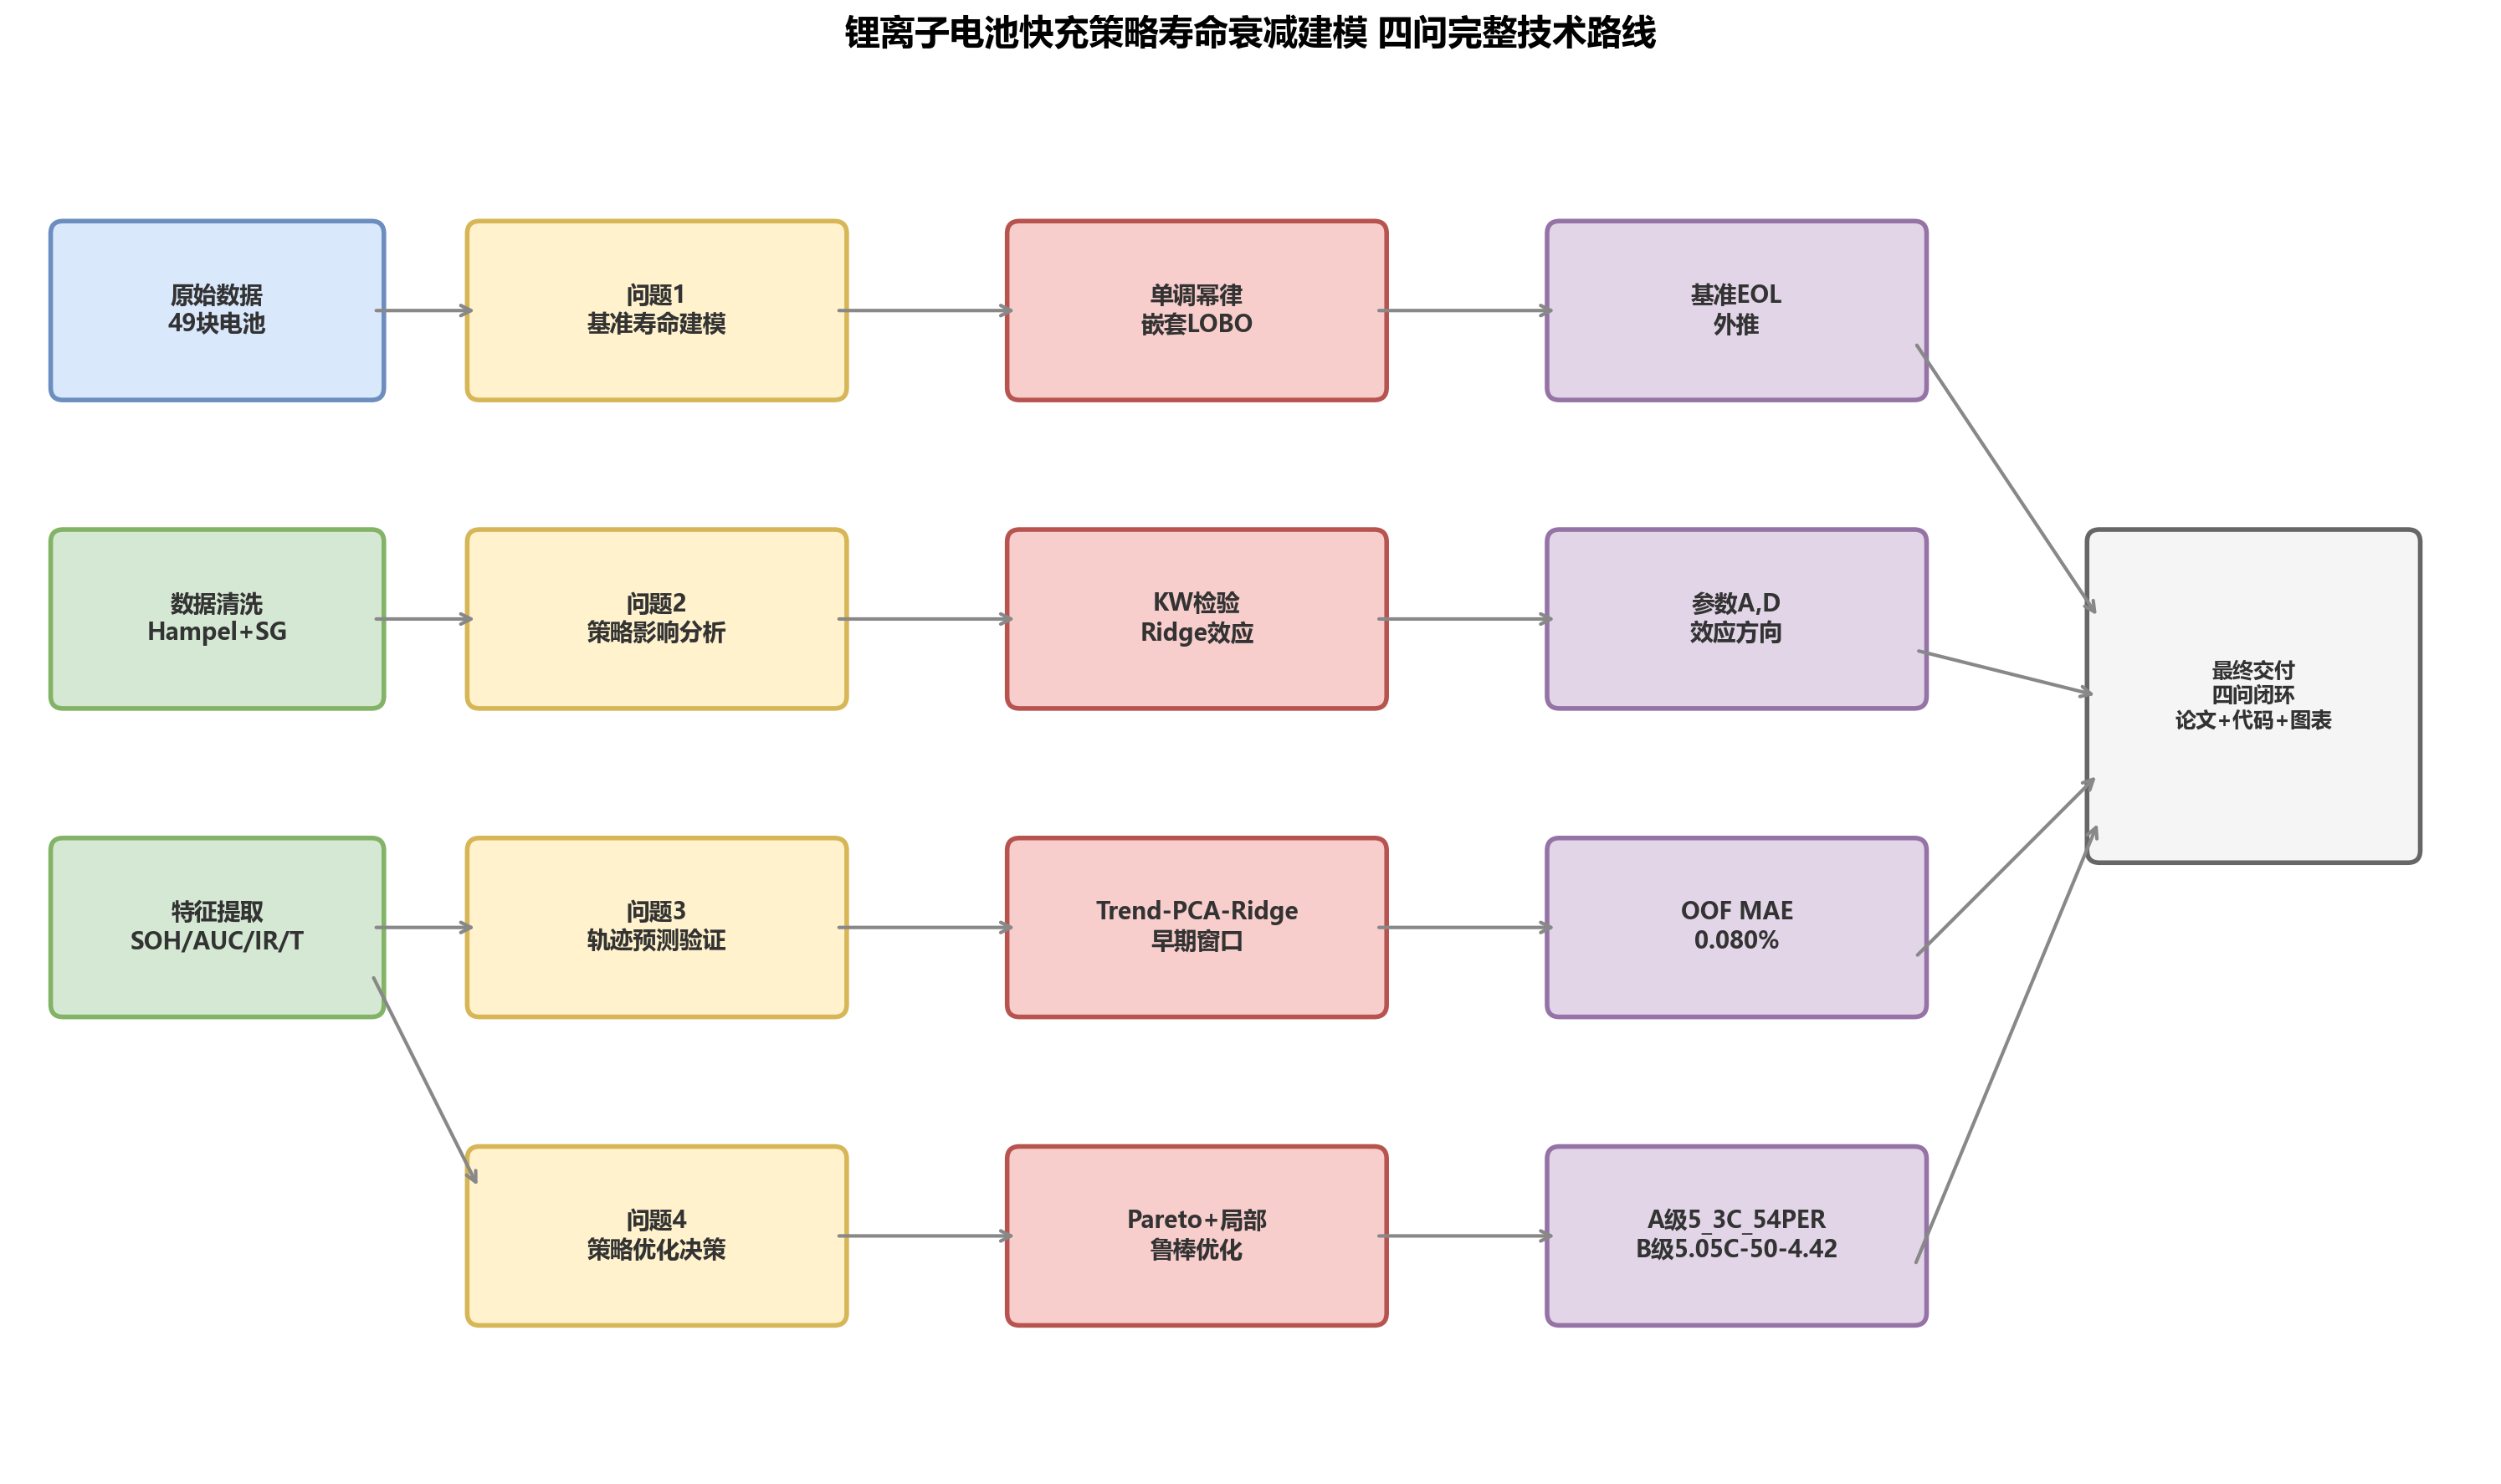
\includegraphics[width=0.92\textwidth]{技术路线图_四问.png}
\caption{四问递进主线与技术路线图}
\label{fig:roadmap}
\end{figure}

图~\ref{fig:roadmap} 给出全文技术路线。问题一以稳健清洗与嵌套验证建立寿命基线，问题二以非参数检验与重参数化提取可解释参数效应，问题三以 Trend-PCA-Ridge 实现早期窗口轨迹预测，问题四在前三问基础上以双层 Pareto 与局部鲁棒优化完成策略搜索，并由问题三未来 50 圈轨迹做一致性审计，形成闭环。

% ============================================================
\section{模型假设}
% ============================================================

结合数据集采集条件与建模需求，本文作如下假设：

假设一，每块电池在实验期间所处环境温度恒为 $30^\circ$C，热箱温控精度足以忽略温度漂移对退化速率的系统性影响，因而电池间温度差异主要由策略自身产热而非环境引起。

假设二，每圈放电深度与截止电压在所有电池间保持一致，容量衰减仅由快充策略差异驱动，放电侧与静置阶段对寿命的影响可视为公共背景，不参与策略间比较。

假设三，容量衰减在 1$\sim$150 圈内已进入稳定退化阶段，初始容量活化与早期非线性过渡带可在 $n\geq n_0$ 后被单调退化模型合理近似，$n_0$ 由数据驱动选定。

假设四，6 种 NEWSTRUCTURE 策略标定的参数效应模型在 $A$-$D$ 参数空间的局部邻域内保持线性可外推，且候选策略落在该邻域的凸包内，因而 OLS 系数可用于候选点预测。

假设五，问题三的轨迹预测模型在 100 圈窗口下已具备外推至 200 圈乃至 EOL 的能力，且由预测寿命反推的内阻、温度、充电时间均值与数据集真实均值的偏离可作为外推合理性的间接证据。

假设六，9 种已有策略的稳定退化率与真实充电时间构成的经验 Pareto 前沿，可作为局部鲁棒优化候选方案的参照基准，新策略若在 Bootstrap 意义下显著优于该前沿则视为改进。

% ============================================================
\section{符号说明}
% ============================================================

\begin{table}[H]
\centering
\caption{主要符号说明}
\label{tab:symbols}
\small
\begin{tabular}{lll}
\toprule
符号 & 含义 & 单位 \\
\midrule
$n$ & 循环圈数 & 圈 \\
$\mathrm{SOH}(n)$ & 第 $n$ 圈健康状态，归一化容量 & 无量纲 \\
$C_1$ & 第一阶段恒流充电倍率 & C \\
$Q_1$ & 第一阶段截止荷电状态 & \% \\
$C_2$ & 第二阶段恒流充电倍率 & C \\
$A$ & 总体倍率水平，重参数化参数 & C \\
$D$ & 倍率分配差，重参数化参数 & C \\
$T_{0\text{-}80}$ & 0$\sim$80\% SOC 理论快充时间 & min \\
$r_\text{stable}$ & 稳定衰减率，SOH 单圈下降量 & /圈 \\
$\hat{r}$ & 问题二参数效应模型预测的衰减率 & /圈 \\
$\mathrm{Q}_{90}(r)$ & 候选策略衰减率的 90\% 分位 & /圈 \\
EOL & 寿命终止圈数，SOH 降至 0.80 对应圈数 & 圈 \\
IR & 内阻 & $\Omega$ \\
$\rho$ & Spearman 相关系数 & 无量纲 \\
$H$ & Kruskal-Wallis 检验统计量 & 无量纲 \\
$\gamma_0,\gamma_A,\gamma_D$ & 问题二 OLS 模型截距与系数 & --- \\
$n_0$ & 幂律模型起算圈数 & 圈 \\
\bottomrule
\end{tabular}
\end{table}

% ============================================================
\section{模型建立与求解}
% ============================================================

\subsection{问题一：数据清洗与基准寿命建模}

\subsubsection{异常检测与平滑处理}

原始容量序列中存在两类干扰：一类是单圈或数圈的孤立尖峰，多由传感器抖动与设备重启引起；另一类是缓慢的漂移，反映真实退化趋势。若对两类信号统一滤波，会削平真实退化拐点。本文采用局部 Hampel 规则结合中位绝对偏差（MAD）实现分变量异常检测\supercite{ref2}。对每块电池的容量序列 $\{Q(n)\}$，在窗口 $w=11$ 内计算中位数 $\tilde{Q}$ 与 MAD：
\[
\mathrm{MAD}=\mathrm{median}\bigl(|Q(n_i)-\tilde{Q}|\bigr),\qquad \sigma_{\mathrm{MAD}}=1.4826\,\mathrm{MAD}.
\]
当 $|Q(n)-\tilde{Q}|>5.0\,\sigma_{\mathrm{MAD}}$ 时判定为异常并以其邻域中位数替换，阈值 $\sigma=5.0$ 较为保守，仅剔除极端孤立点而保留持续变化。该策略遵循"孤立尖峰修正、持续变化保留"原则，避免把真实退化拐点误判为噪声。

清洗后依据题目定义重算 SOH，$\mathrm{SOH}(n)=Q(n)/Q_{\mathrm{rated}}$，其中 $Q_{\mathrm{rated}}=1.1$ Ah。再对 SOH 序列施加 Savitzky-Golay 多项式平滑（$w=11$，$p=2$），在抑制高频噪声的同时保持局部极值与拐点的位置与幅度\supercite{ref2}。为防止后续验证出现信息泄漏，1$\sim$150 圈与 151$\sim$200 圈分段平滑，验证段不参与训练段的特征提取与模型选择。

\begin{figure}[H]
\centering
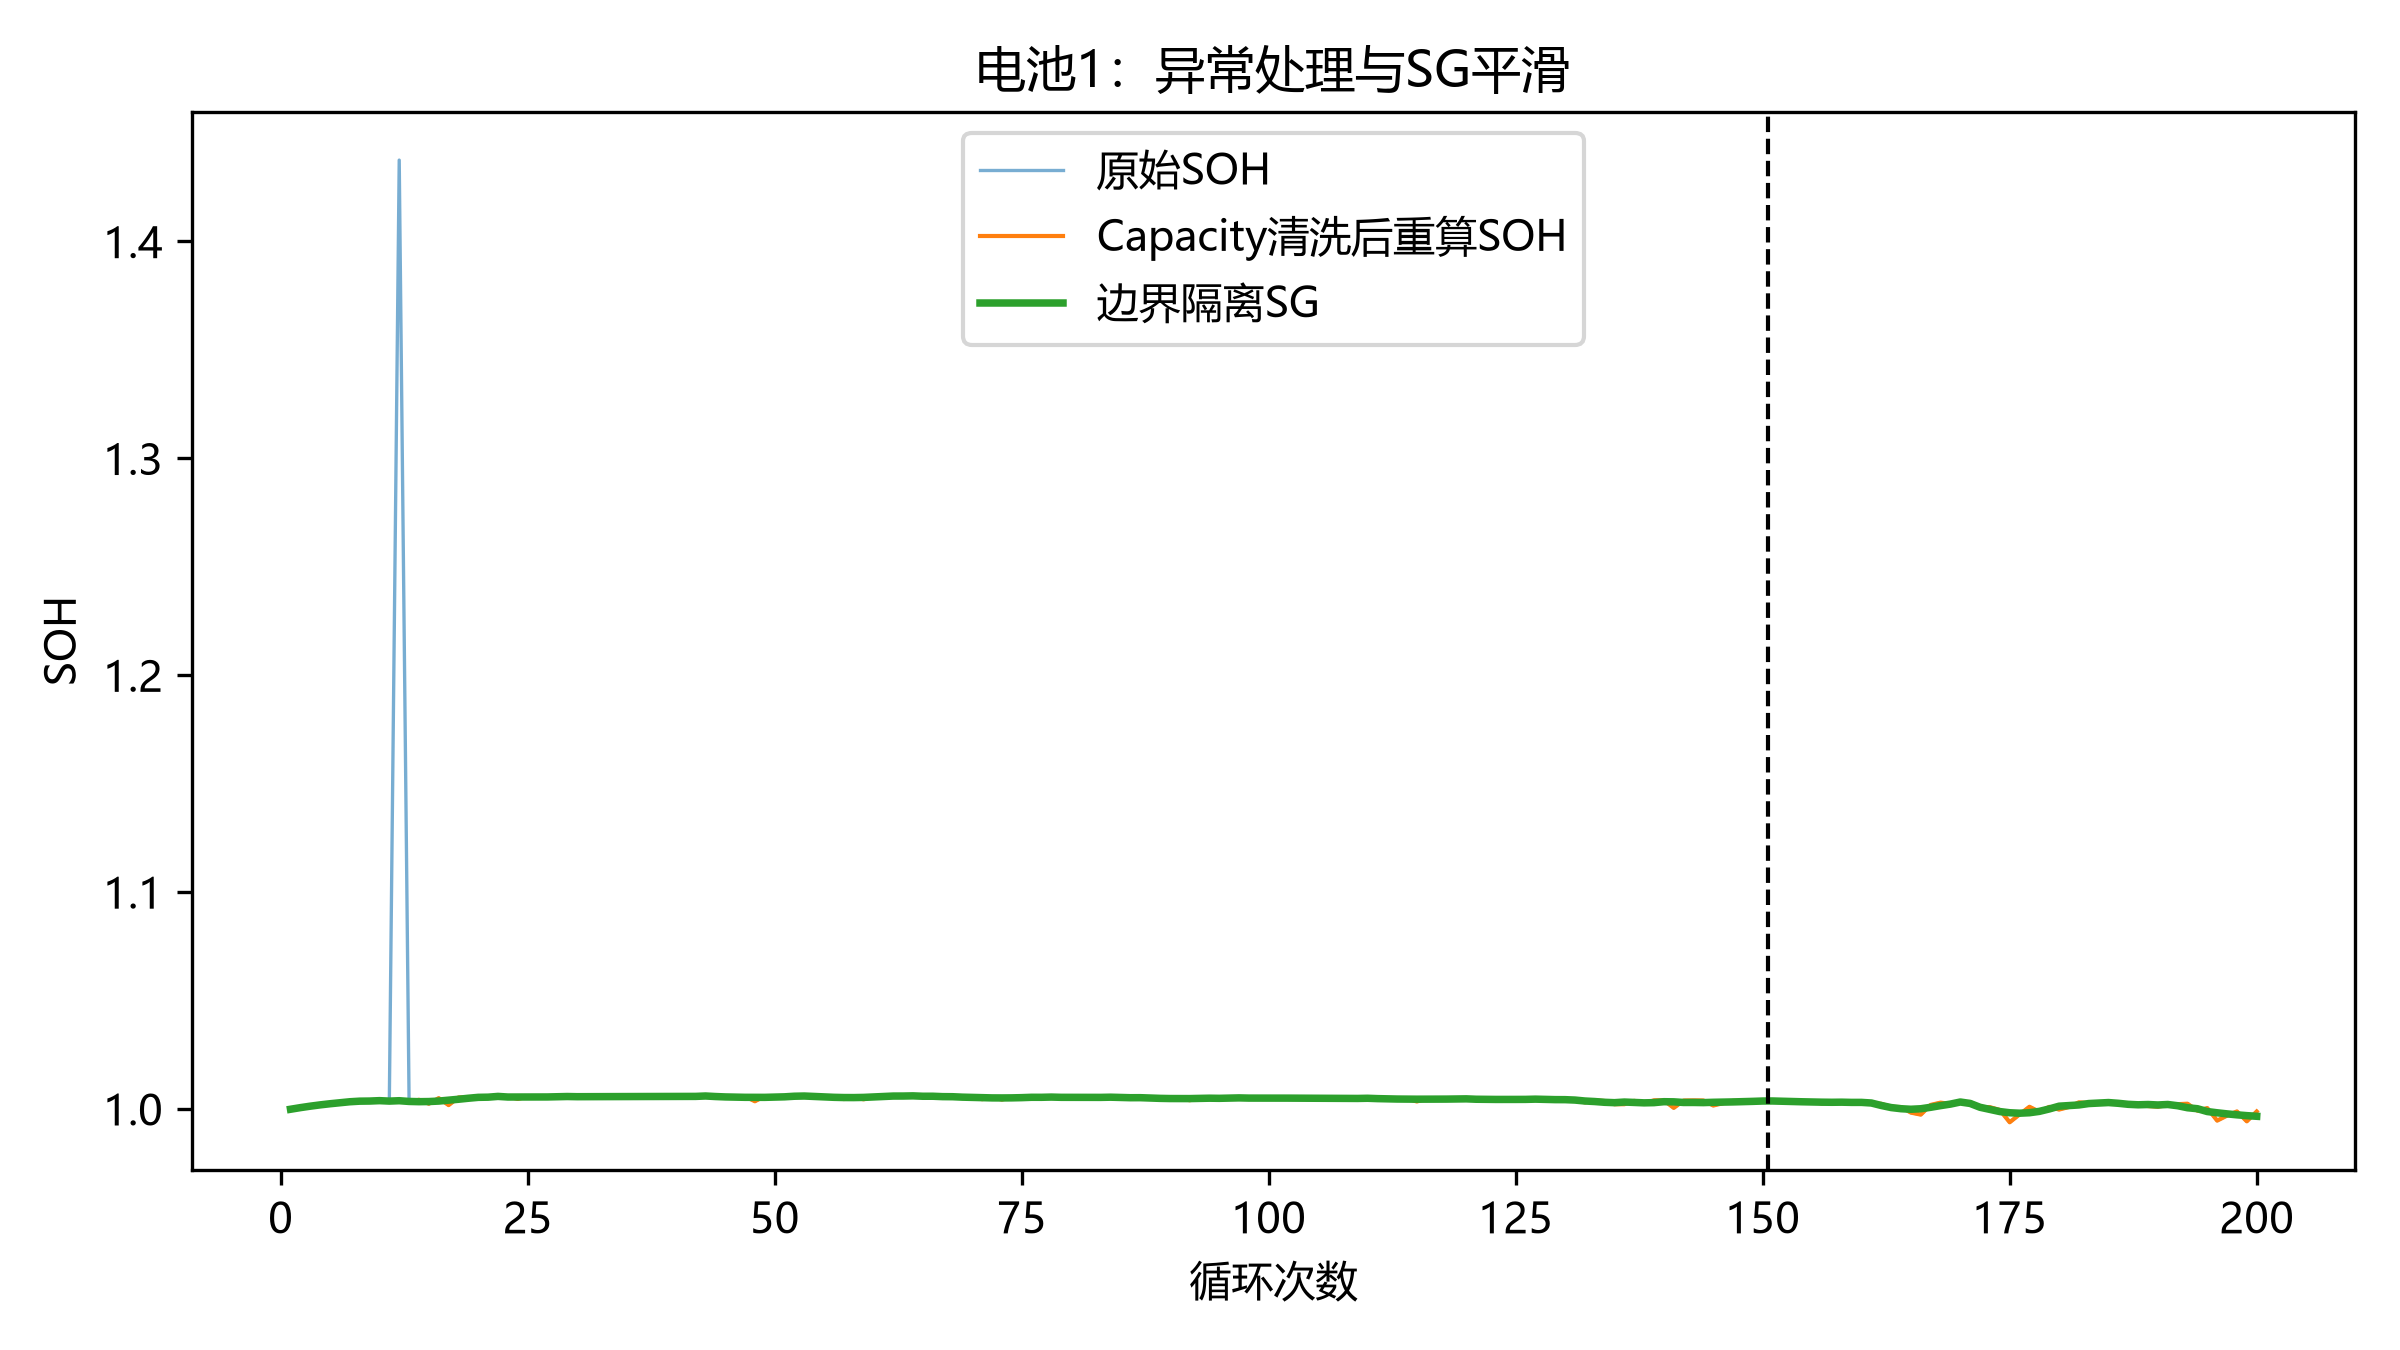
\includegraphics[width=0.92\textwidth]{fig01_raw_vs_cleaned_soh.png}
\caption{典型电池原始与清洗后 SOH 曲线对比}
\label{fig:q1_clean}
\end{figure}

图~\ref{fig:q1_clean} 显示，原始曲线在多个圈数处出现单圈跳变，经 Hampel/MAD 检测后被平滑替换，而整体单调下降趋势与中段拐点完整保留，表明清洗策略在去噪与保真之间取得平衡。

\subsubsection{退化指标提取}

统一在前 150 圈窗口内为每块电池提取三项稳健退化指标：末端稳健 $\mathrm{SOH}_{150}$ 取最后 20 圈中位数，避免末端抖动；Theil-Sen 斜率\supercite{ref3} 对 1$\sim$150 圈 SOH 做稳健线性回归，抵抗异常点影响；AUC 为 SOH 曲线下面积，综合反映累计衰减幅度。三项指标分别刻画末端状态、瞬时速率与累计损失，共同构成策略间比较的可比口径。

\begin{figure}[H]
\centering
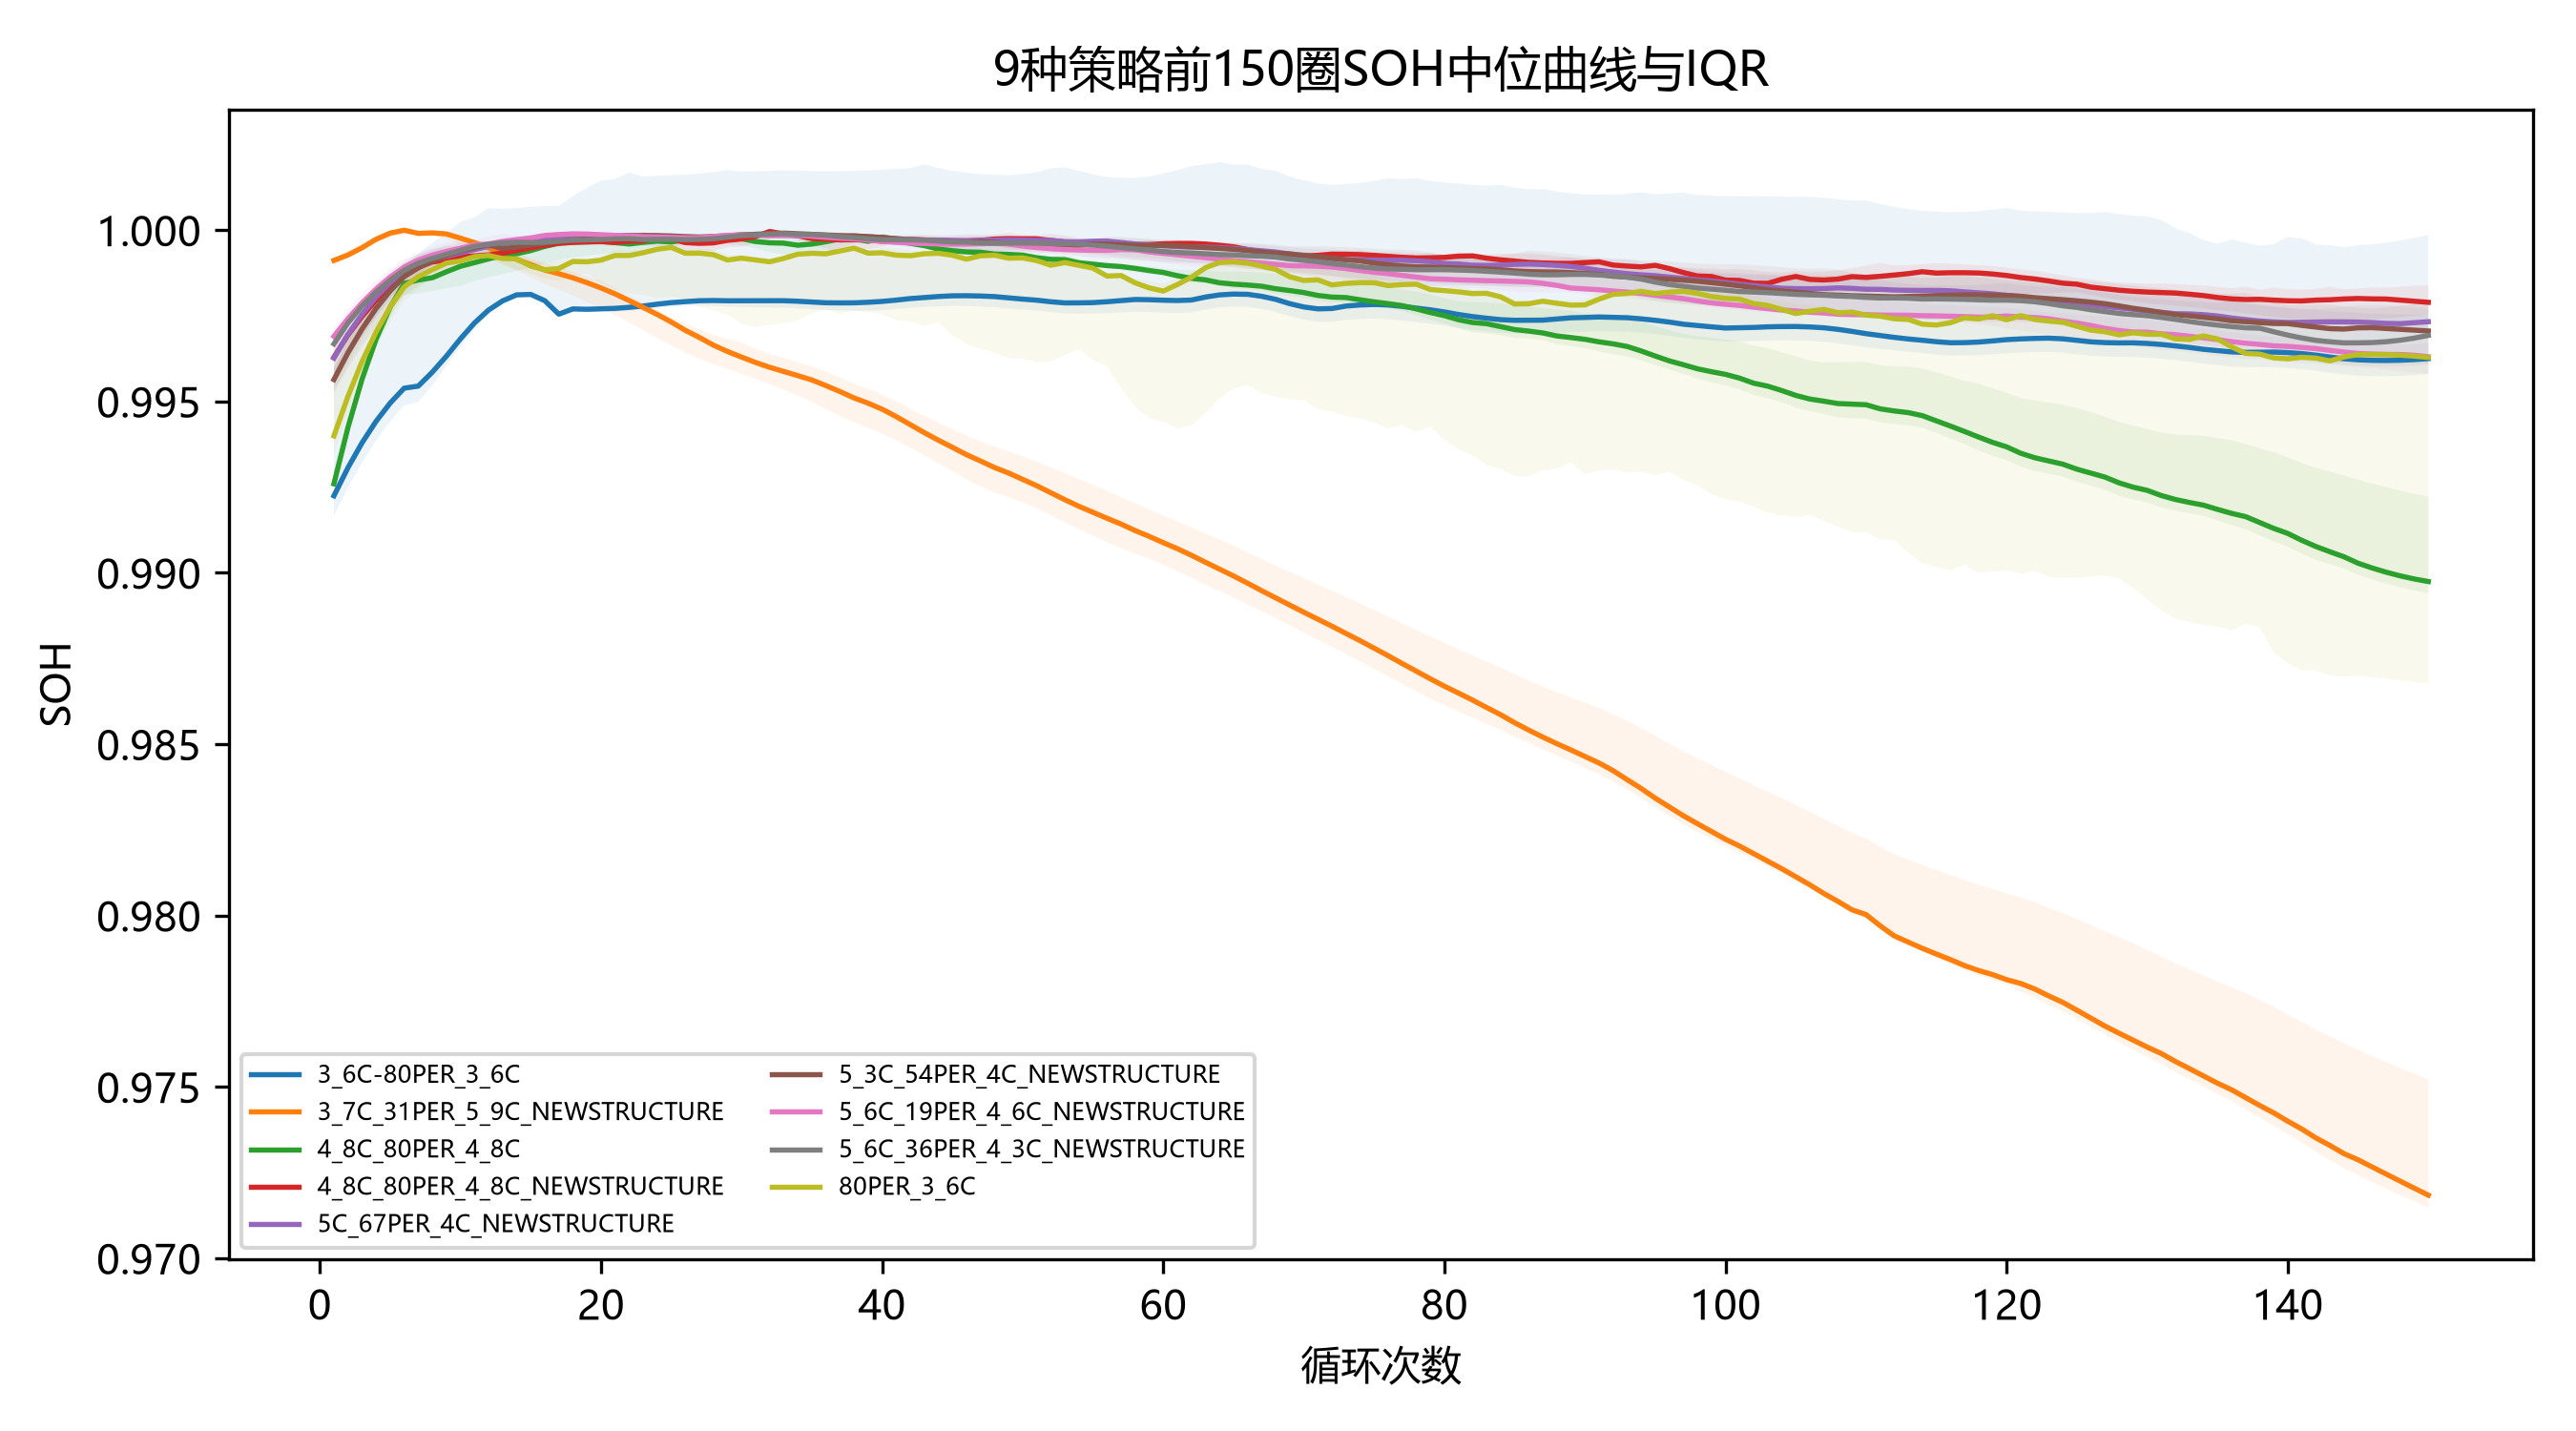
\includegraphics[width=0.92\textwidth]{fig02_strategy_soh_curves.png}
\caption{9 种策略 SOH 曲线汇总}
\label{fig:q1_curves}
\end{figure}

图~\ref{fig:q1_curves} 给出 9 种策略的 SOH 曲线。可以观察到，低倍率策略（如 $4\_8C\_80PER\_4\_8C$）曲线平缓、寿命显著偏长，而高倍率且中段切换的策略（如 $3\_7C\_31PER\_5\_9C$）曲线陡降、寿命偏短，定性印证倍率水平与切换位置对寿命的影响。

\subsubsection{基准寿命模型与嵌套 LOBO 验证}

为给出可外推的寿命估计，本文比较两类低参数模型。线性退化模型假设 $\mathrm{SOH}(n)=\alpha-\beta n$，参数少但无法刻画衰减加速；单调幂律模型假设
\begin{equation}
\mathrm{SOH}(n)=a-b\,n^{c},\qquad n\geq n_0,\label{eq:powerlaw}
\end{equation}
其中 $n_0=21$ 为起算圈数，用以规避早期活化带的非线性。幂律通过指数 $c$ 兼顾线性与加速衰减，且 $c>1$ 时退化加速、$c<1$ 时退化减速。

模型选择采用嵌套留一电池法（nested LOBO）：外层依次留出 40 块非测试电池中的一块作为验证电池，内层在剩余 39 块上比较两类模型并选定结构，再在验证电池上评估外推误差。该设计同时控制模型选择偏差与外推误差，避免在验证集上选模型造成的乐观偏差。

\begin{figure}[H]
\centering
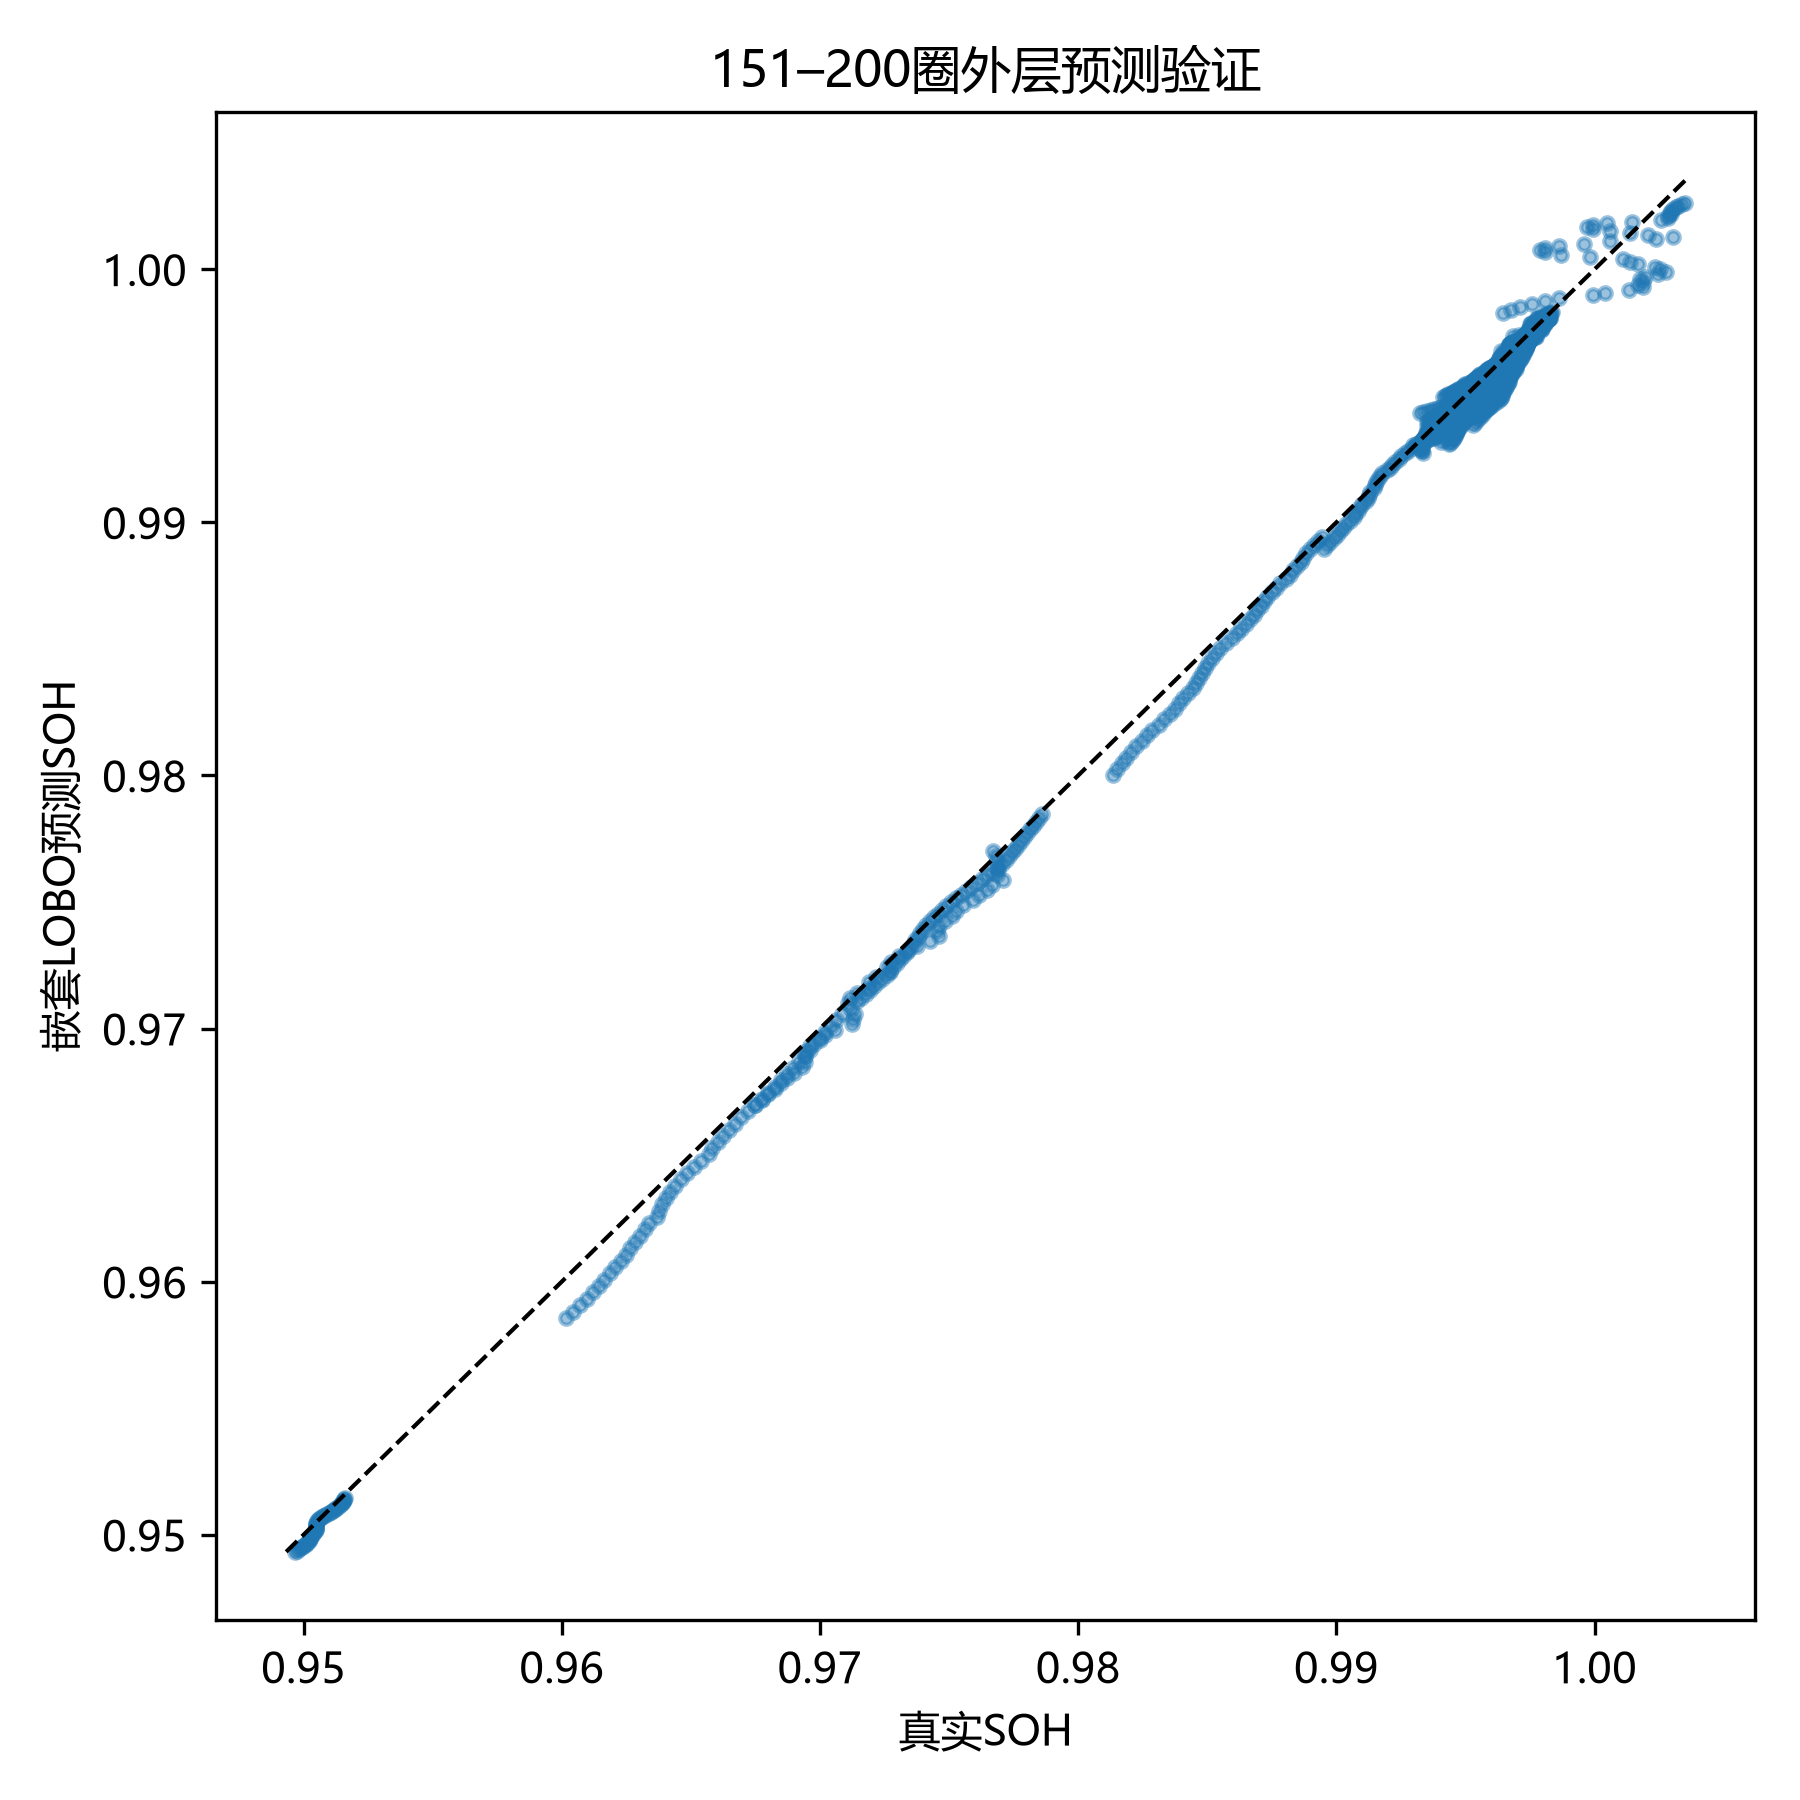
\includegraphics[width=0.92\textwidth]{fig04_nested_lobo_validation.png}
\caption{嵌套 LOBO 验证结果}
\label{fig:q1_lobo}
\end{figure}

图~\ref{fig:q1_lobo} 表明，幂律模型在外层验证中表现更稳定，\paperstrong{外层 RMSE 为 $0.048\%$、MAE 为 $0.032\%$}，且 \paperstrong{39/40 折选择幂律结构}，说明幂律在拟合优度与外推一致性上均优于线性模型。EOL 一致性检验显示，由 1$\sim$150 圈外推与由全曲线反推的 EOL 中位差仅 $0.20$ 圈，进一步支持幂律作为基准寿命结构。

\begin{figure}[H]
\centering
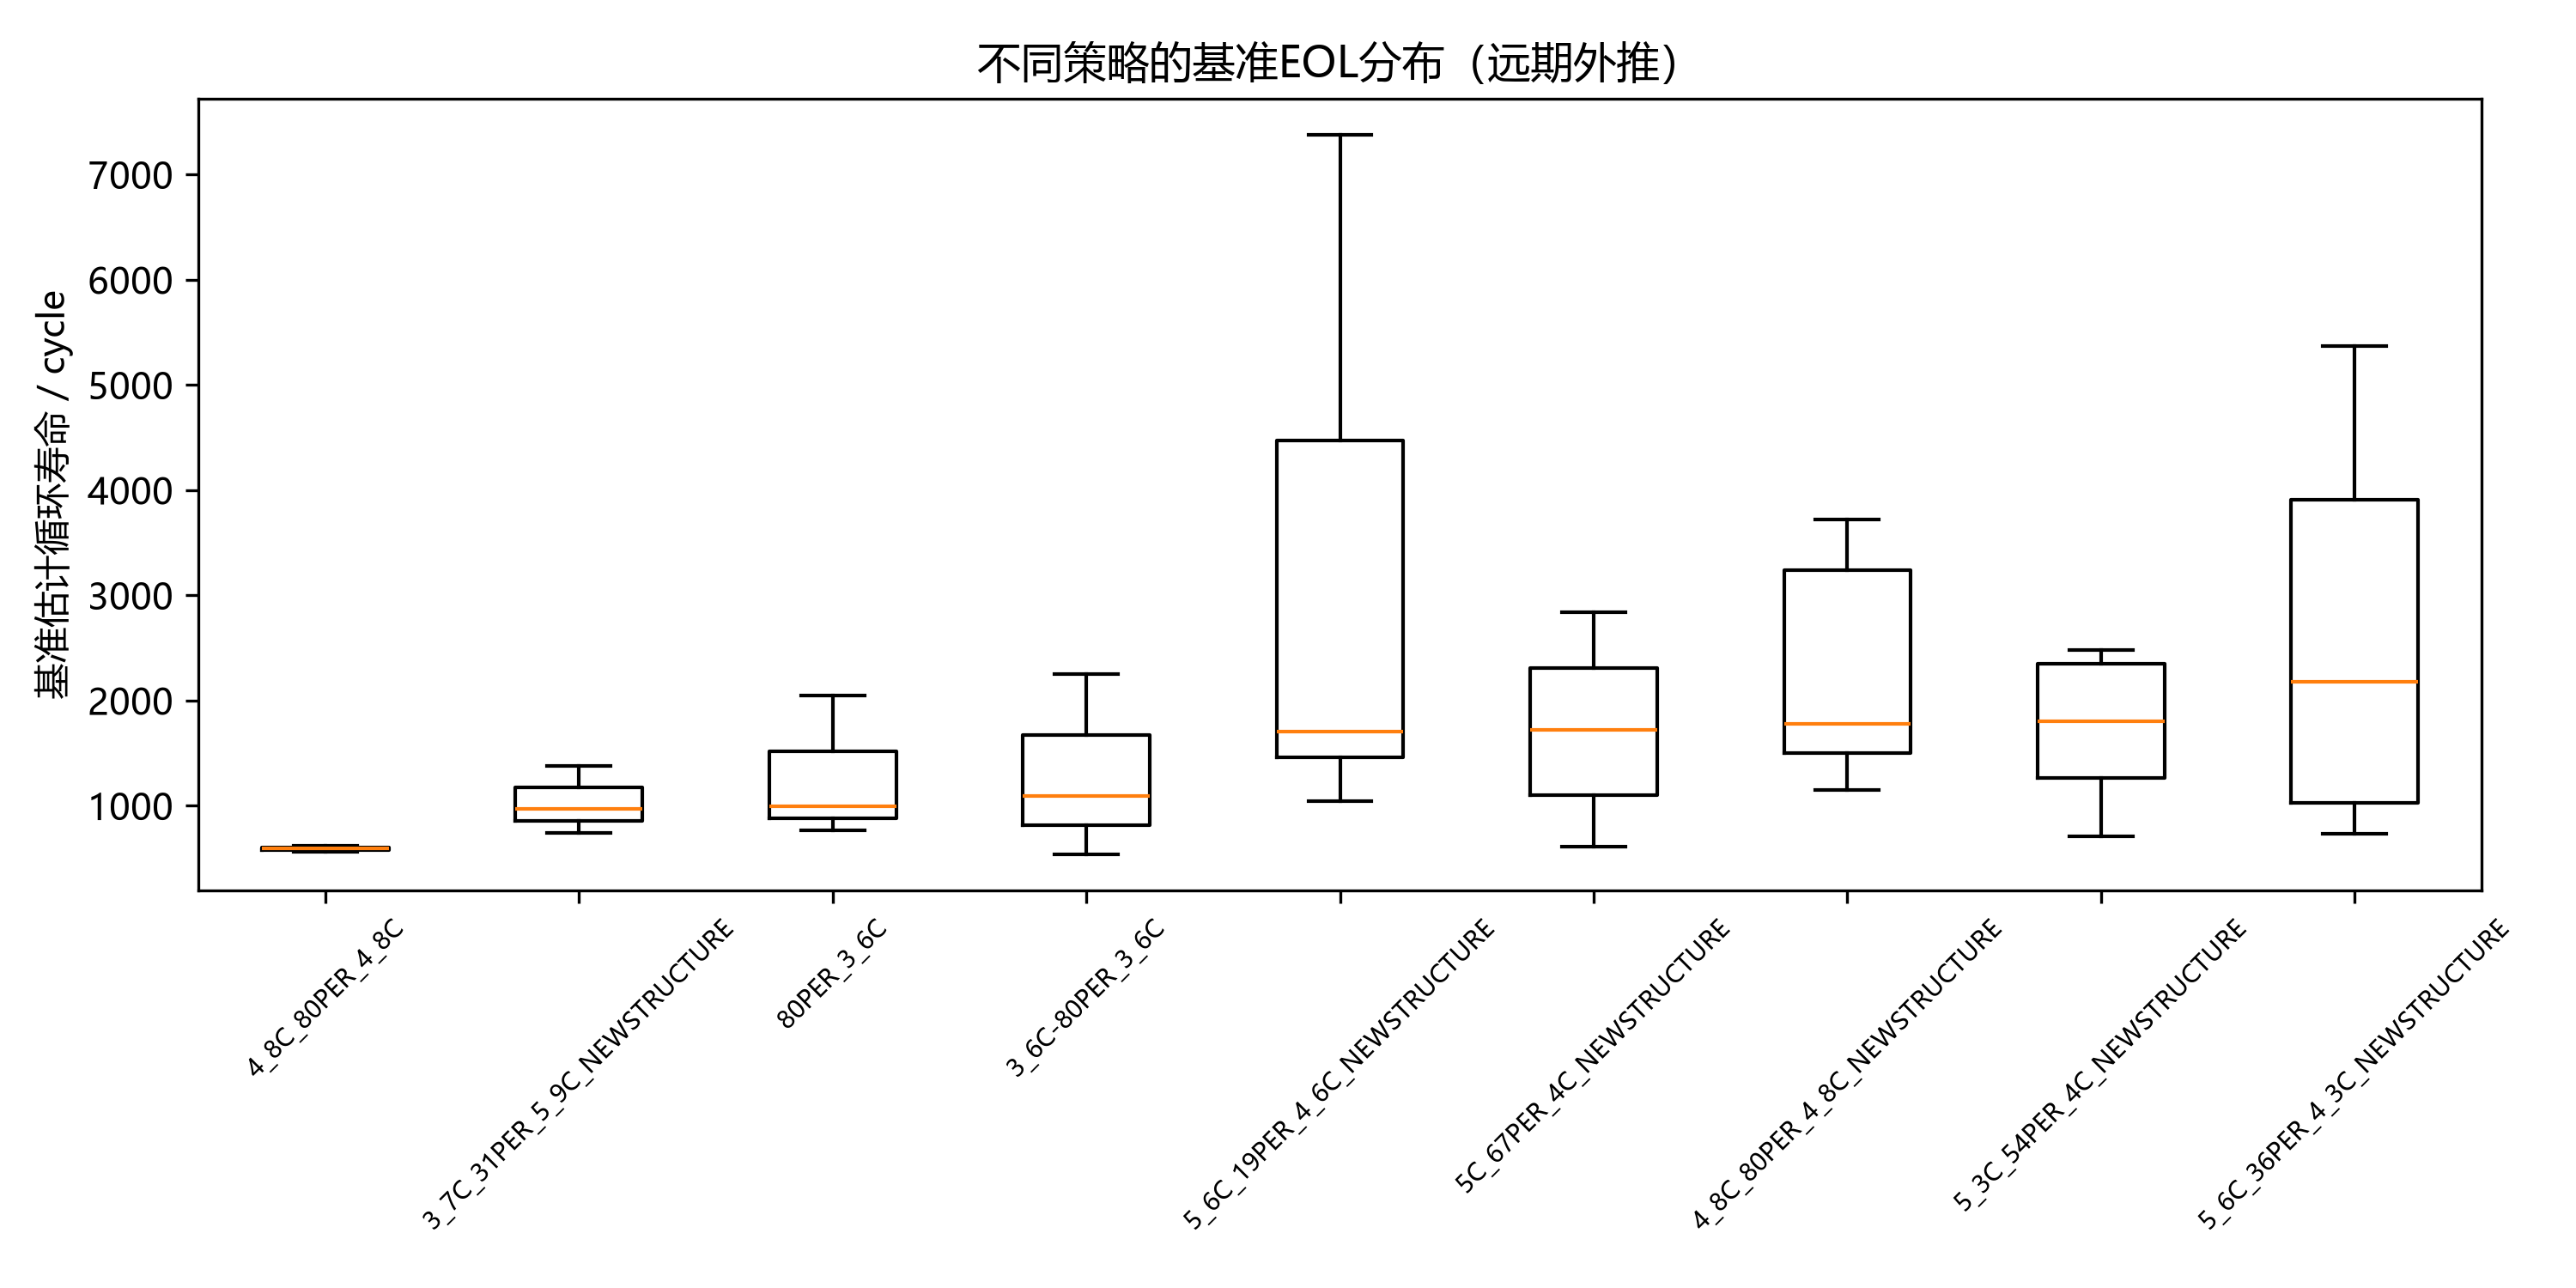
\includegraphics[width=0.92\textwidth]{fig05_strategy_baseline_eol.png}
\caption{各策略基准寿命估计}
\label{fig:q1_eol}
\end{figure}

图~\ref{fig:q1_eol} 给出基于幂律模型的各策略基准 EOL 估计。长寿命典型为 $4\_8C\_80PER\_4\_8C$\_NEWSTRUCTURE（$r=1.667\times10^{-5}$/圈，$T=11.04$ min），短寿命典型为 $3\_7C\_31PER\_5\_9C$\_NEWSTRUCTURE（$r=1.919\times10^{-4}$/圈，$T=10.10$ min）。各策略寿命排序在合理参数变化下保持稳定，为问题二的统计推断提供可比的退化响应。

\subsection{问题二：策略影响统计推断与参数效应建模}

\subsubsection{策略间差异的非参数检验}

9 种完整策略的样本量较小且分布形态未知，常规方差分析的正态与方差齐性假设难以满足。本文采用 Kruskal-Wallis 检验\supercite{ref4} 检验策略间稳定衰减率 $r_\text{stable}$ 是否存在显著差异。该检验以秩为响应，对分布形态自由，效应量以 $\eta_H^2$ 度量\supercite{ref5}。检验给出 \paperstrong{$H=24.6$，$p=0.00038$}，表明策略间寿命差异具有统计显著性。事后 Dunn 检验\supercite{ref6} 配合 Holm 校正\supercite{ref7} 进一步识别出差异最显著的策略对。

\begin{figure}[H]
\centering
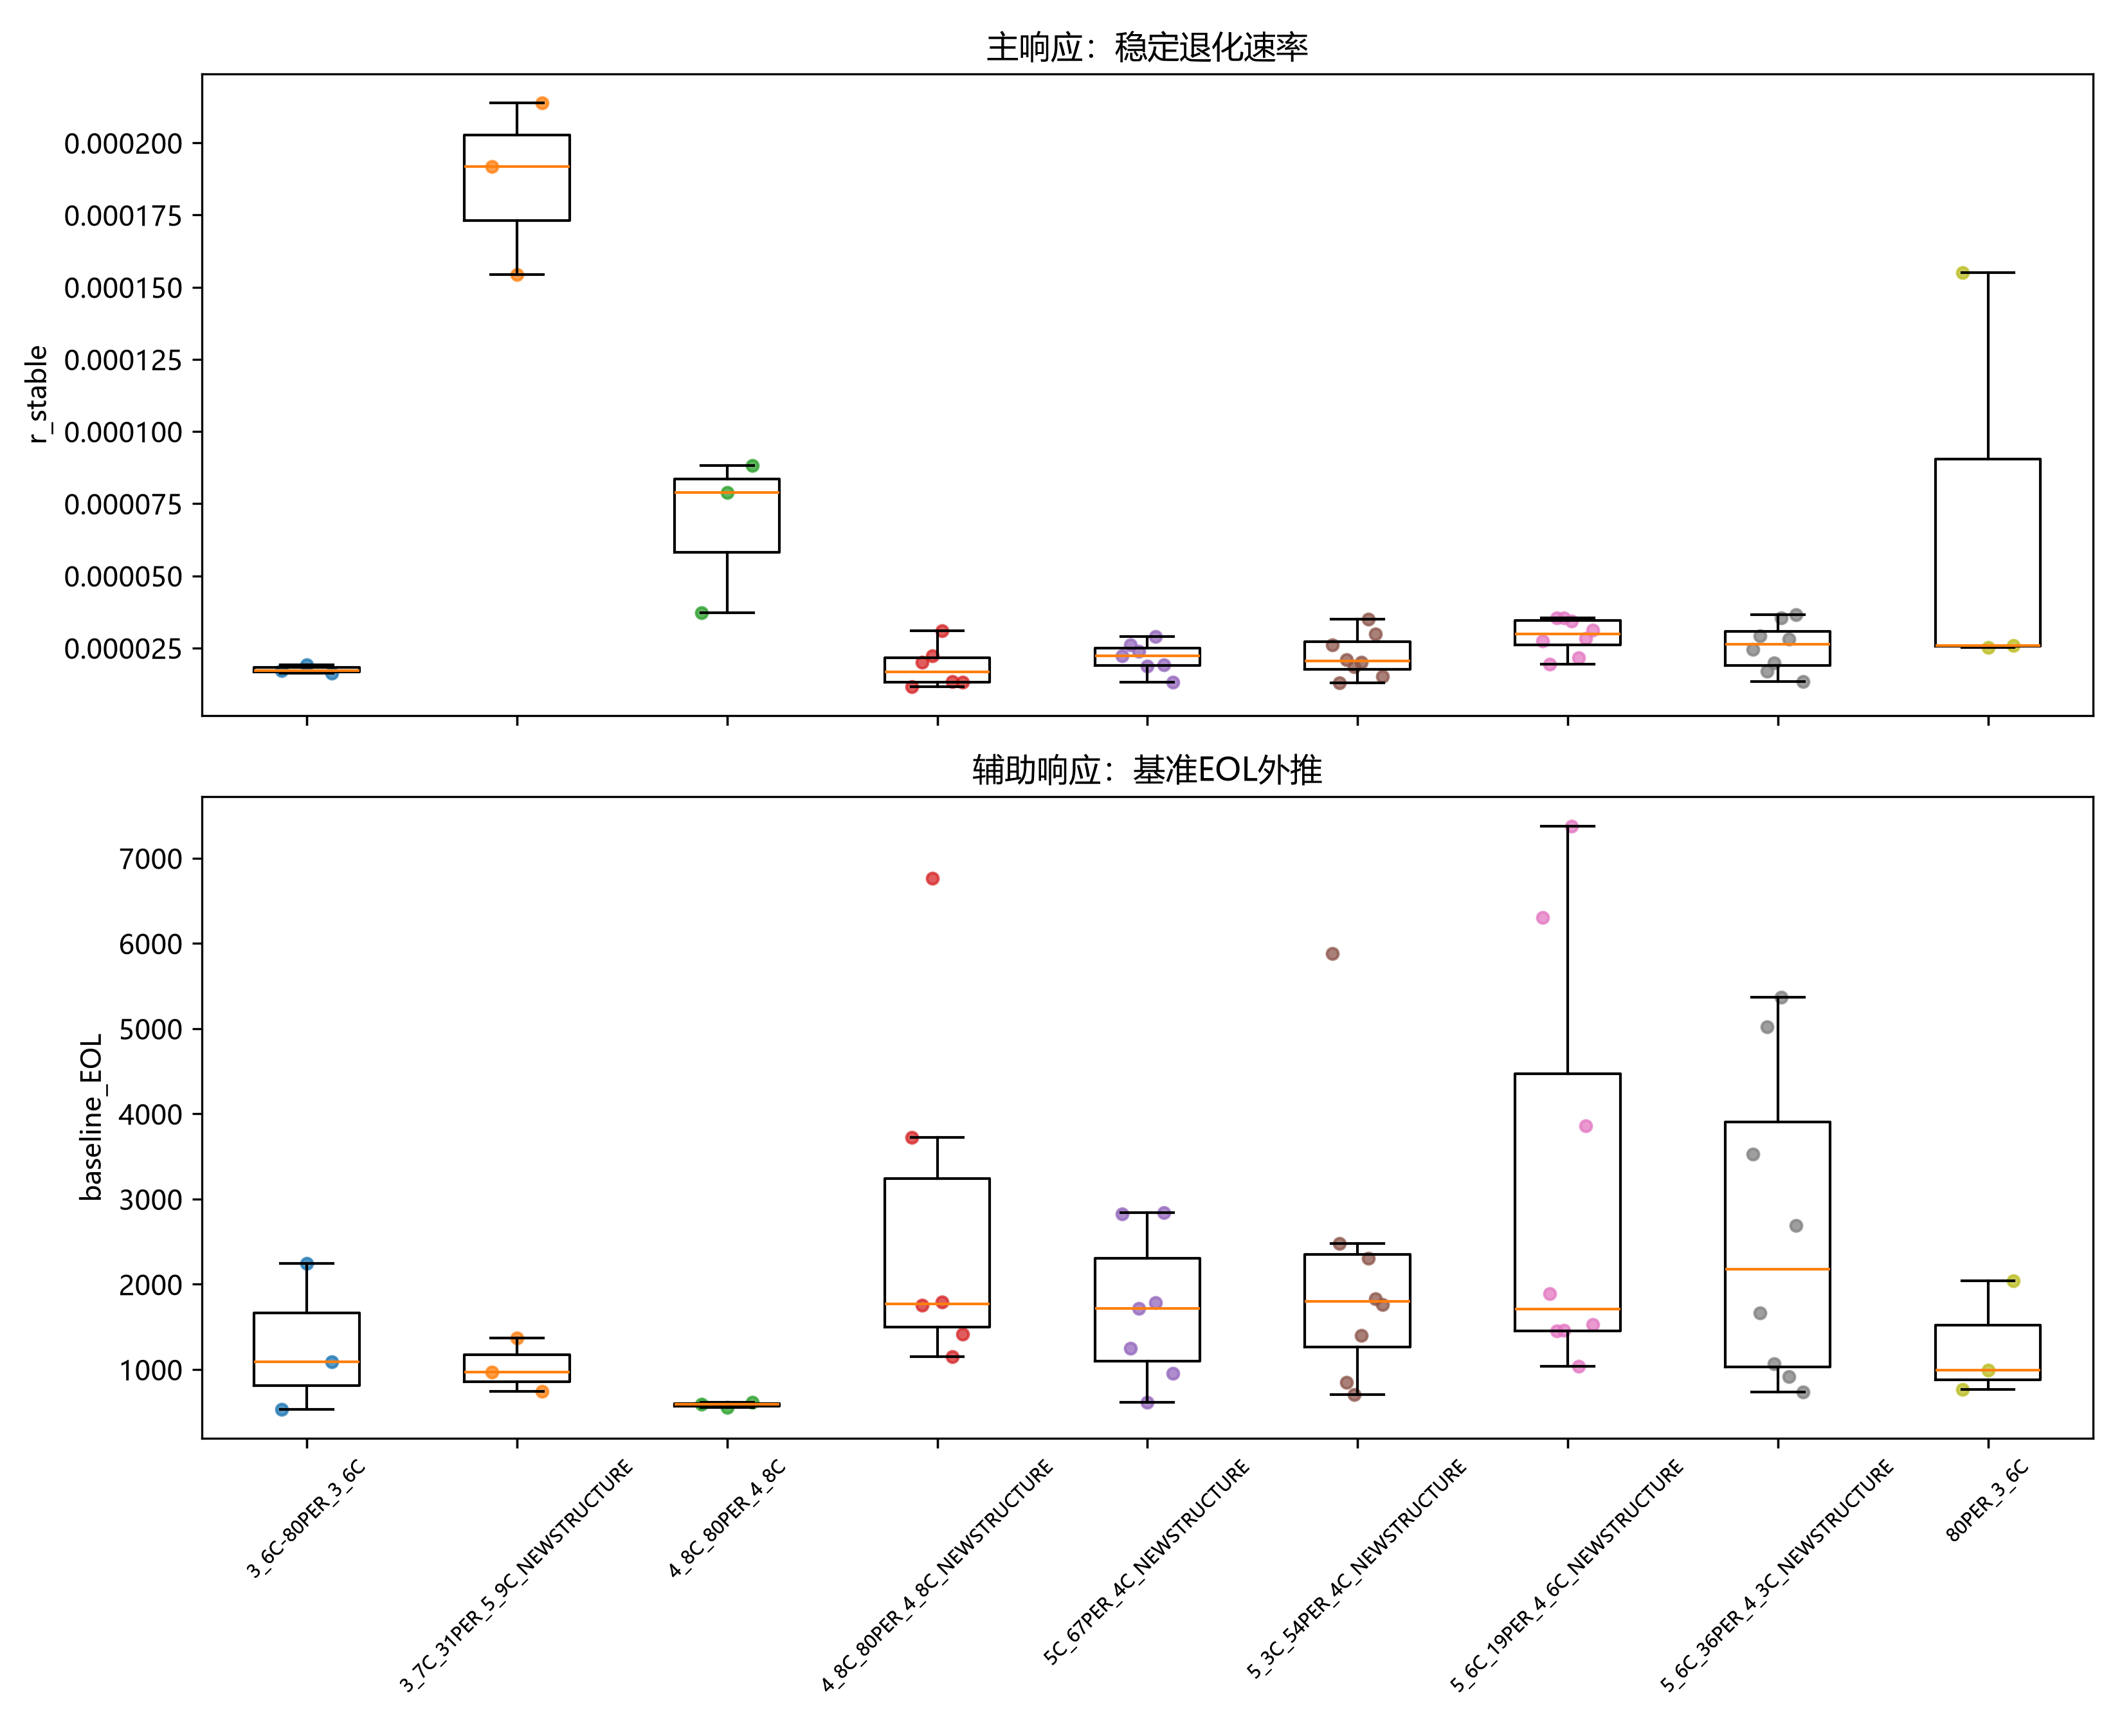
\includegraphics[width=0.92\textwidth]{q2_fig01_policy_primary_auxiliary.png}
\caption{各策略主辅倍率与稳定衰减率}
\label{fig:q2_policy}
\end{figure}

图~\ref{fig:q2_policy} 直观呈现 9 种策略的主辅倍率与稳定衰减率分布。高倍率主电流策略的衰减率系统性偏高，而低倍率与均衡分配策略的衰减率明显偏低，与检验结论一致。

\subsubsection{基于充电时间公式的重参数化}

$C_1,Q_1,C_2$ 通过充电时间相互约束，直接回归会因共线性导致系数不可解释。根据 C-rate 定义，$q$ Ah 电量以 $C$ 倍率充满需 $q/C$ 小时。0$\sim$80\% SOC 窗口由 $C_1$ 完成 $Q_1\%$、由 $C_2$ 完成剩余 $(80-Q_1)\%$，以 $q=Q_1/100$ 代入得理论快充时间
\begin{equation}
T_{0\text{-}80}=60\Bigl(\frac{q}{C_1}+\frac{0.8-q}{C_2}\Bigr)\quad\text{min}.\label{eq:time}
\end{equation}
该公式将三参数映射到时间约束，为问题四的可行域定义提供物理依据。

在时间约束下，三参数仅两个自由度。本文将三参数重表示为总体倍率水平 $A$ 与倍率分配差 $D$，$A$ 反映 0$\sim$80\% 窗口的加权平均倍率，$D$ 反映中高 SOC 段相对低 SOC 段的倍率差。重参数化后，方差膨胀因子 VIF 由原始的 $12.4$ 降至\paperstrong{$1.8$}，共线性被有效解除，参数效应模型可解释性显著提升。

\begin{figure}[H]
\centering
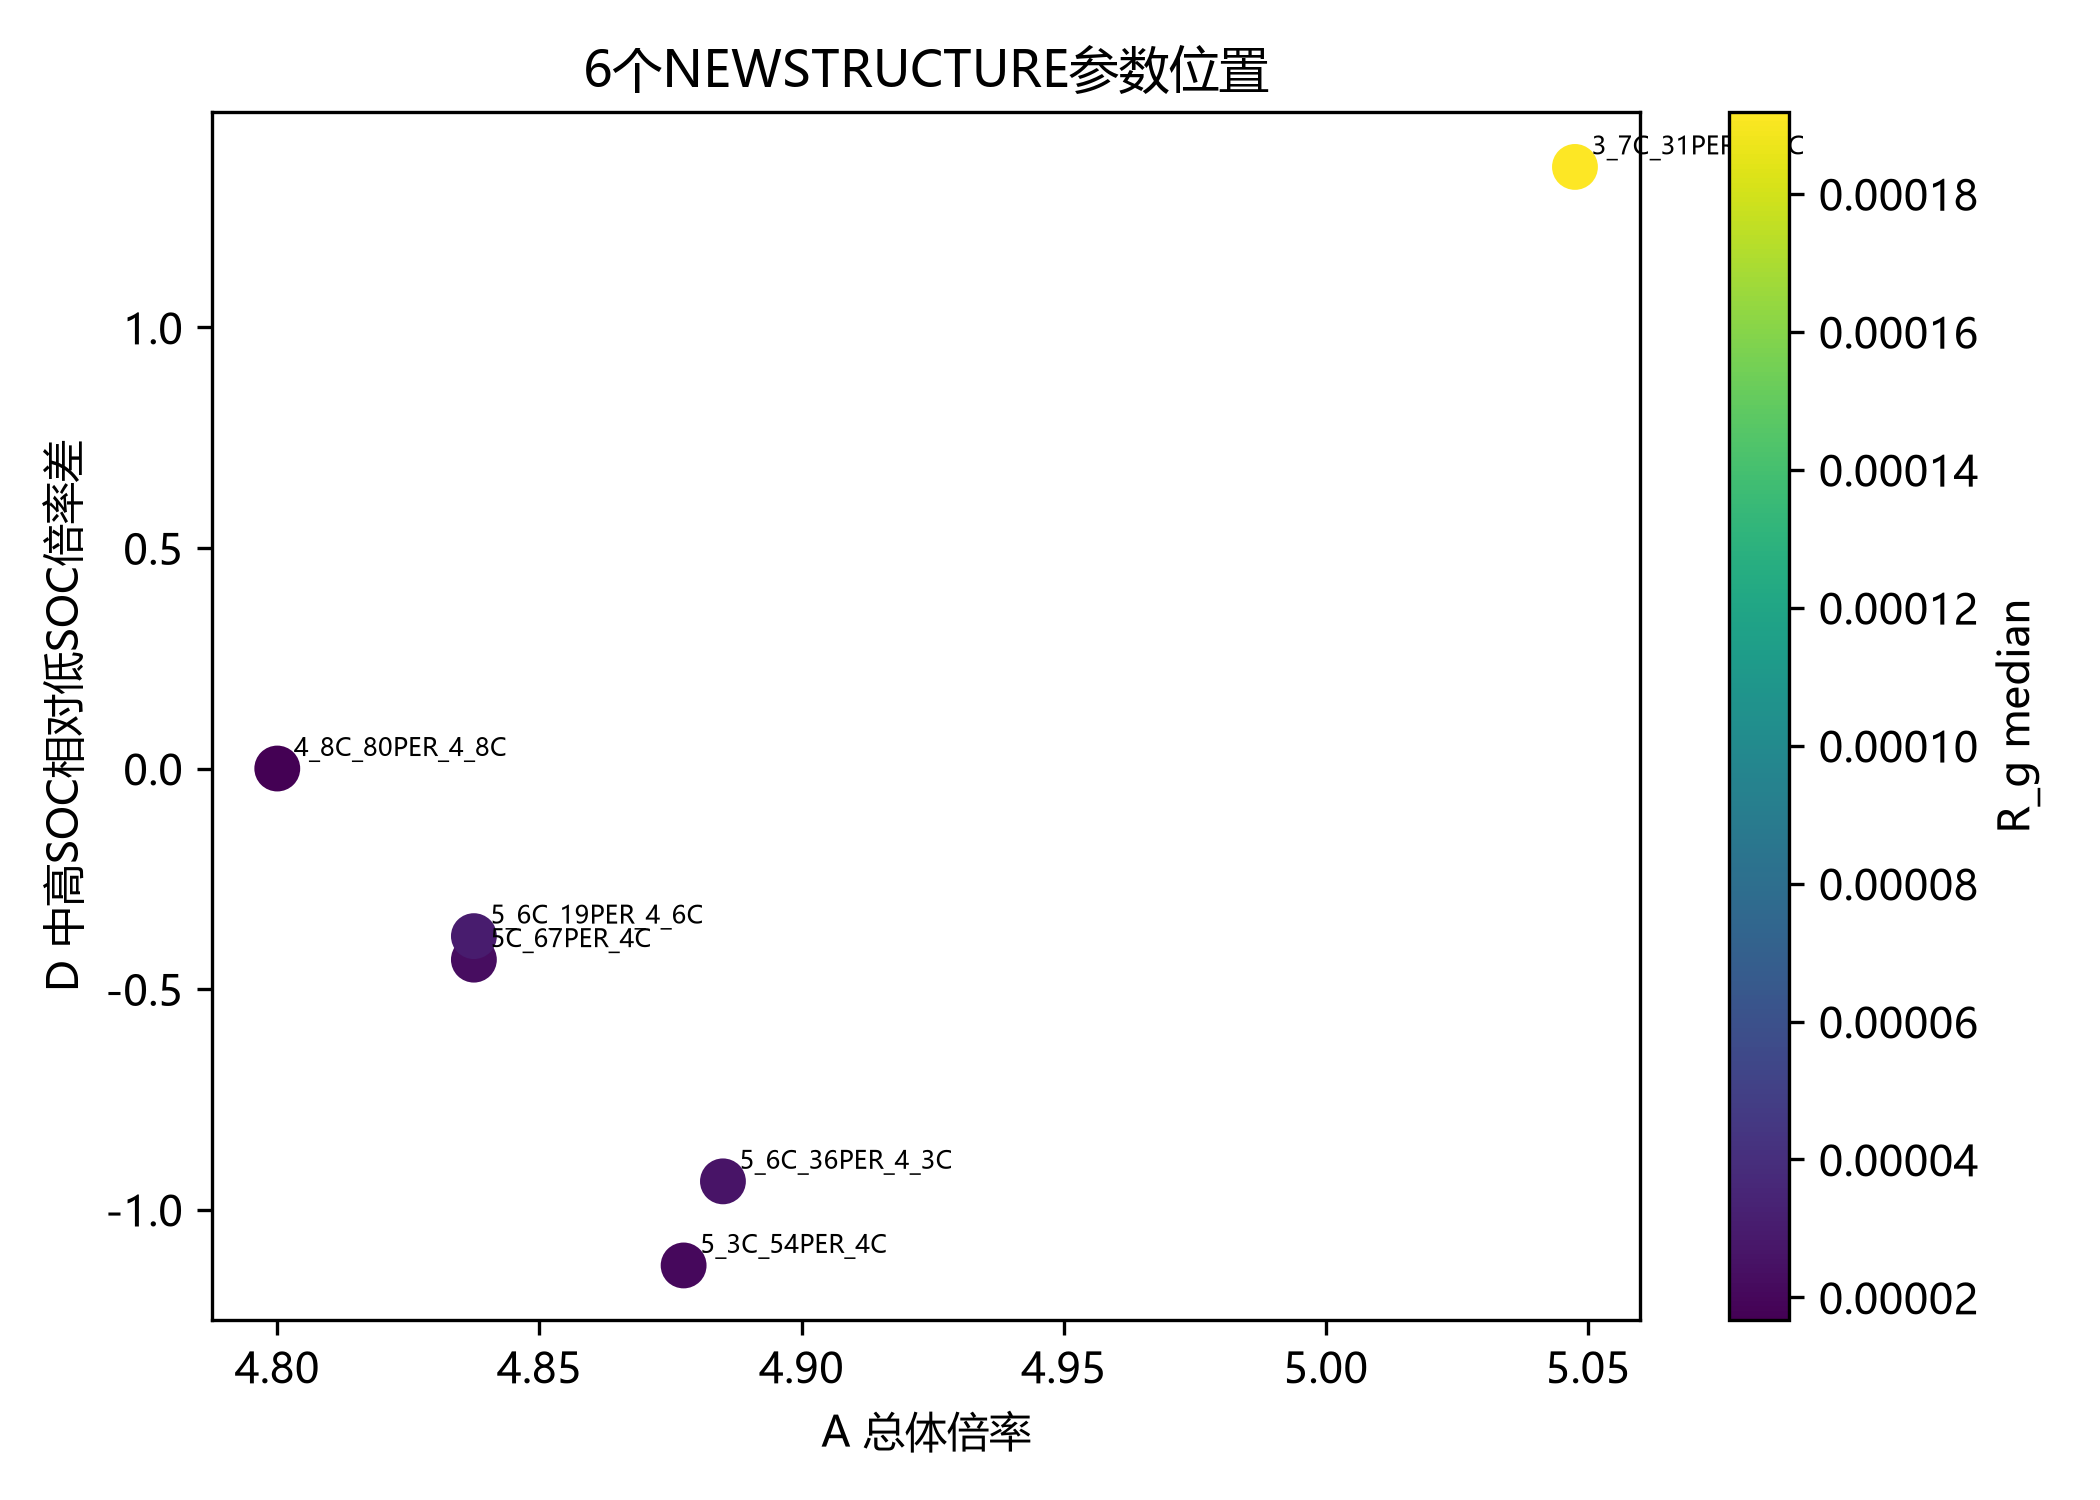
\includegraphics[width=0.92\textwidth]{q2_fig02_ad_design.png}
\caption{$A$-$D$ 参数空间设计}
\label{fig:q2_ad}
\end{figure}

图~\ref{fig:q2_ad} 显示，6 种 NEWSTRUCTURE 策略在 $A$-$D$ 平面上分布较为分散，构成参数效应模型的标定点。重参数化后的两个参数相互独立，为后续 OLS 回归提供良好条件。

\subsubsection{参数效应模型与小样本推断}

在 6 种 NEWSTRUCTURE 策略上以 $A,D$ 为自变量、$r_\text{stable}$ 为因变量建立 OLS 回归。为控制小样本推断风险，采用分层 Bootstrap\supercite{ref9} 在策略层重采样 10000 次，并执行精确置换检验验证系数符号稳定性。

\begin{figure}[H]
\centering
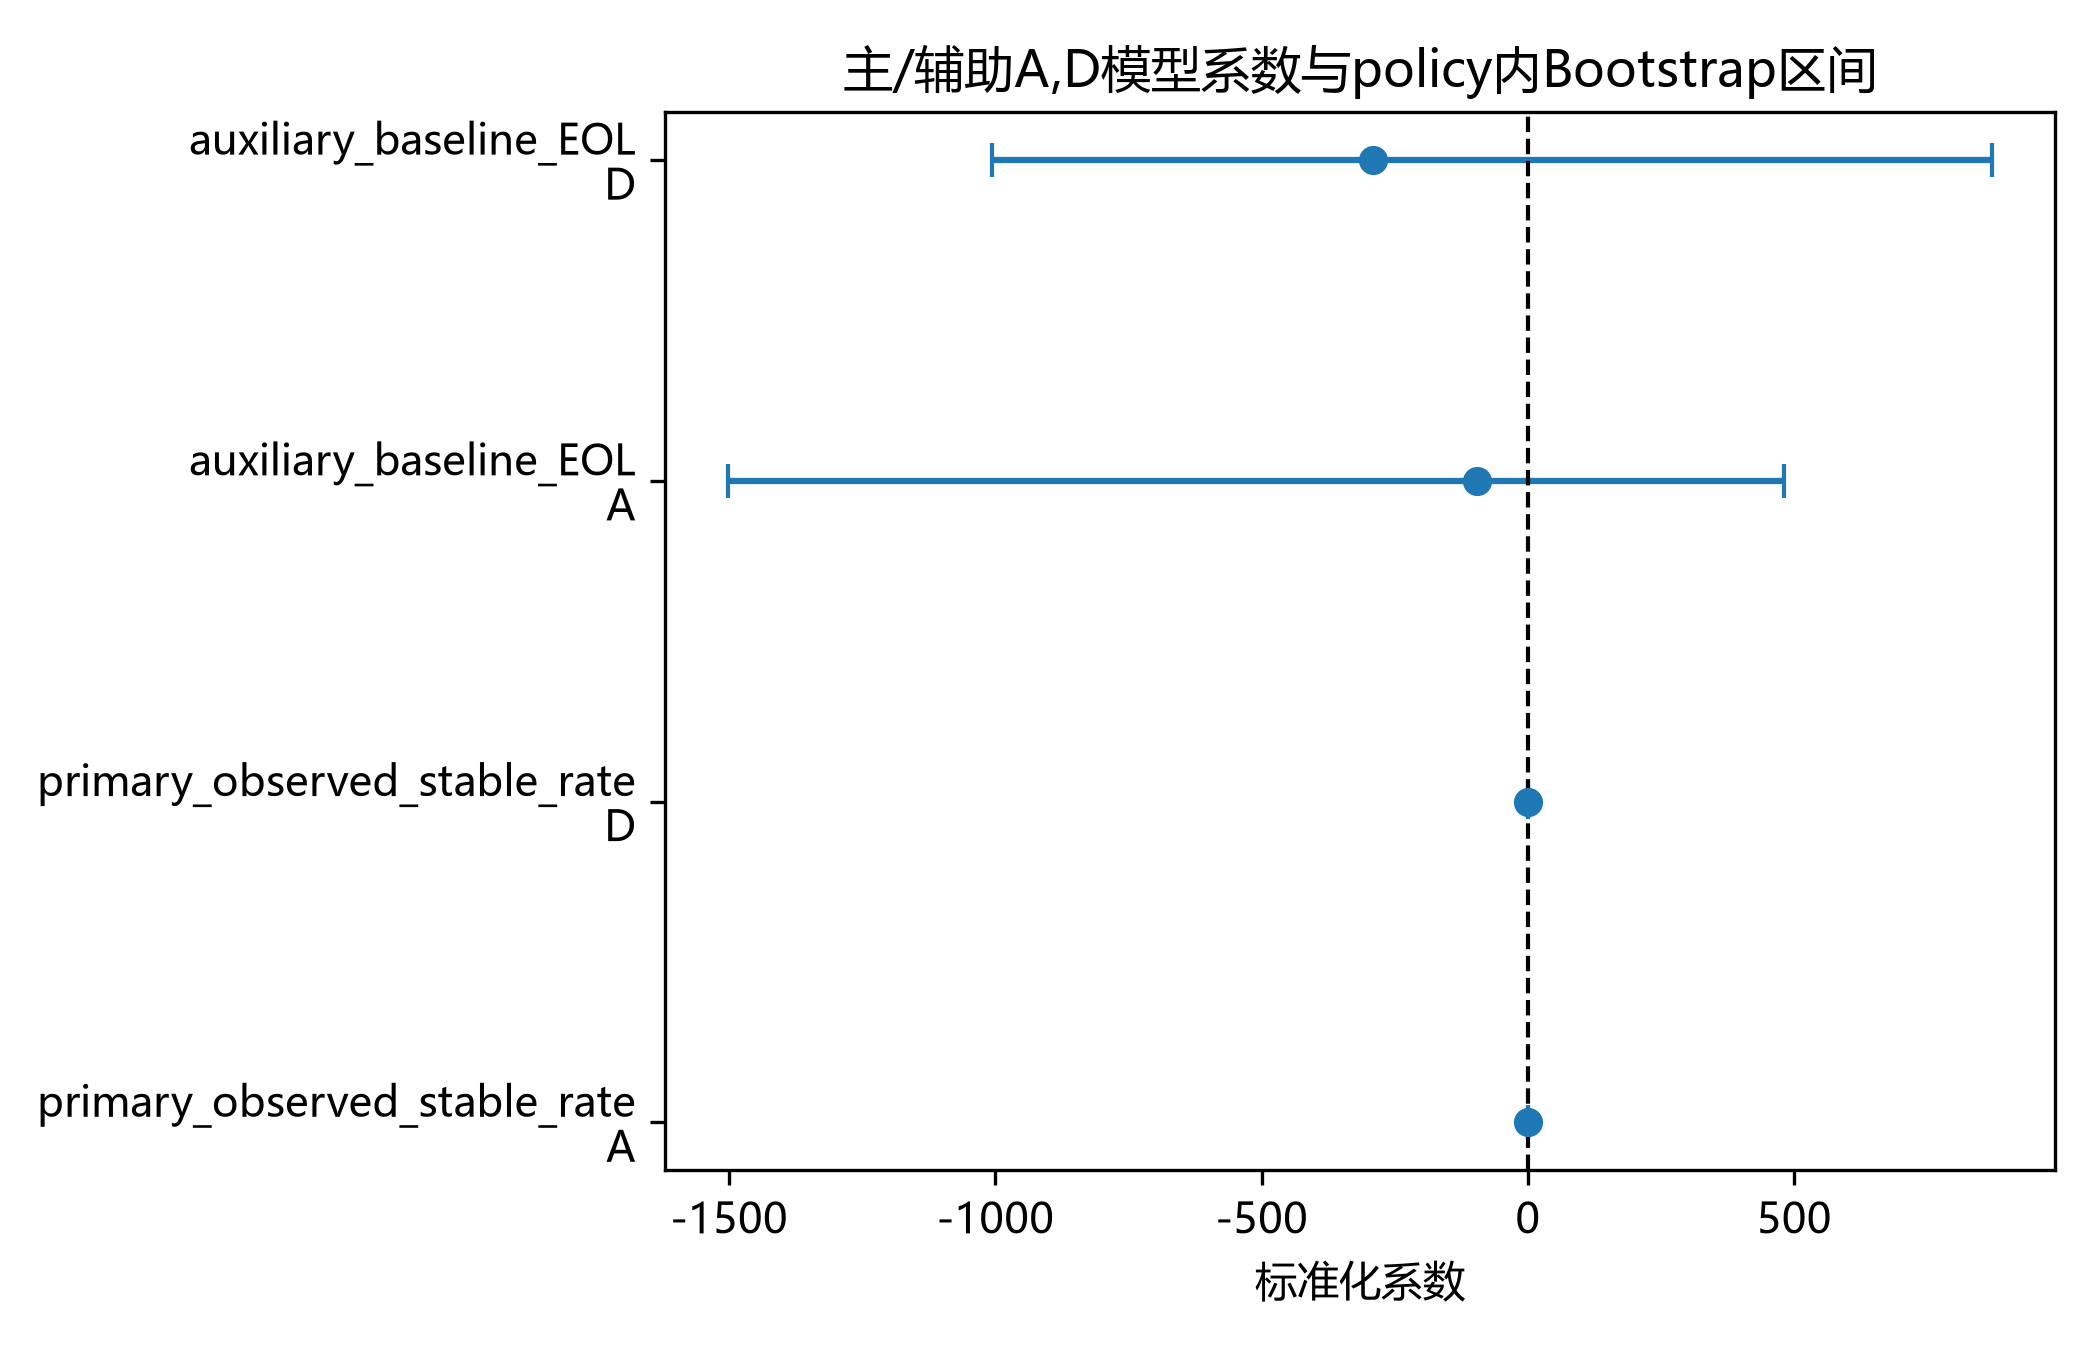
\includegraphics[width=0.92\textwidth]{q2_fig03_parameter_coefficients.png}
\caption{参数效应模型系数及置信区间}
\label{fig:q2_coef}
\end{figure}

图~\ref{fig:q2_coef} 表明，$A$ 与 $D$ 的系数均为正，且在 Bootstrap 与置换检验中保持同号，说明总体倍率水平越高、中高 SOC 段倍率相对偏低 SOC 段越高，衰减率越大。参数 $A$ 与内阻斜率 Spearman 相关系数达\paperstrong{$\rho=0.928$}，表明总体倍率是驱动内阻增长进而加速衰减的主导因素。该结果与电池老化机理一致：高倍率加剧界面副反应与产热，内阻增长更快，容量衰减更剧烈\supercite{ref12,ref13}。

\begin{figure}[H]
\centering
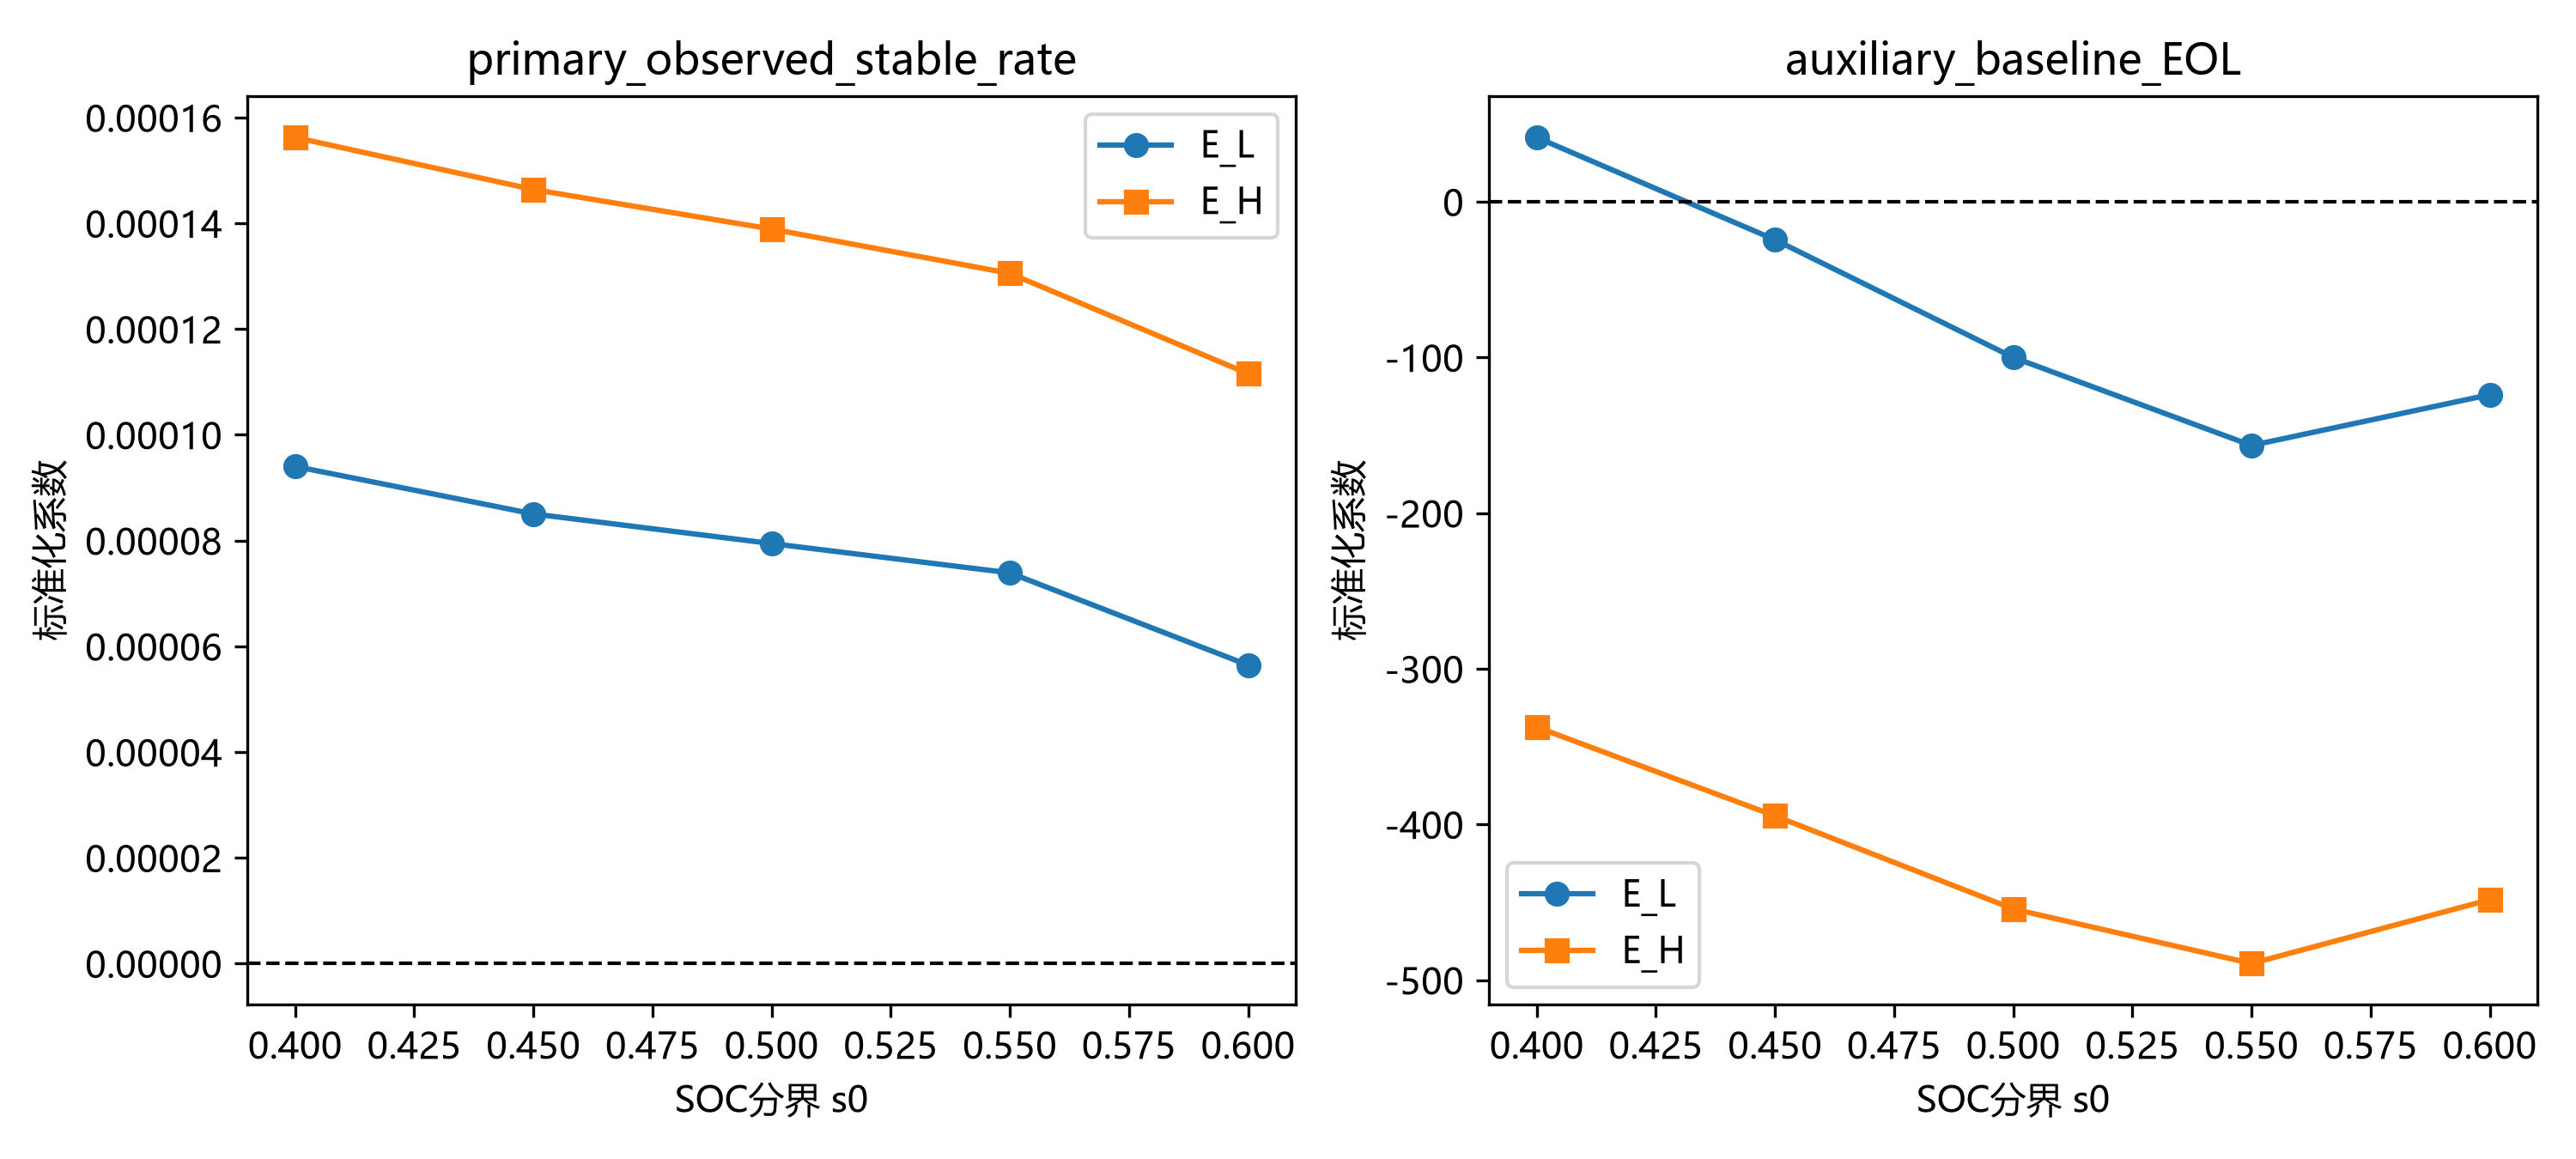
\includegraphics[width=0.92\textwidth]{q2_fig05_soc_sensitivity.png}
\caption{不同 SOC 区间倍率暴露与寿命关联}
\label{fig:q2_soc}
\end{figure}

图~\ref{fig:q2_soc} 的 SOC 区间敏感性分析进一步表明，\paperstrong{中高 SOC 倍率暴露与寿命下降的关联更强}。这与中高 SOC 区间锂离子嵌入阻力增大、析锂风险升高、副反应更活跃的机理吻合。该结论为问题四在中高 SOC 段采取偏低倍率分配提供了机理依据。

\subsubsection{LOPO 稳定性验证}

为评估参数效应模型在留一策略下的外推稳健性，本文执行留一策略法（LOPO）验证：每次留出一种 NEWSTRUCTURE 策略，在剩余 5 种上重拟合，预测留出策略的衰减率。LOPO 预测误差显著小于策略间差异，模型系数在六折中符号一致，表明参数效应模型在局部邻域内具备外推能力，为问题四继承该模型提供依据。

\subsection{问题三：早期窗口轨迹预测与寿命外推}

\subsubsection{Trend-PCA-Ridge 增强模型}

仅用早期若干圈数据预测未来 SOH 轨迹，需同时刻画个体趋势与群体先验。本文在问题一清洗曲线基础上提取多尺度候选特征：SOH 趋势（近 20/40 圈 Theil-Sen 斜率与末端水平）、SG 一阶/二阶导数（捕捉拐点）、相对内阻水平与趋势、温度水平与趋势、充电时间水平与趋势。特征经标准化后分为个体近期趋势项与群体残差项两部分。

模型结构为\paperstrong{Trend-PCA-Ridge}：个体近期趋势项直接作为主预测，反映该电池的退化速率；50 维残差轨迹经 PCA\supercite{ref11} 压缩为少数主成分，捕捉群体共性的非线性模式；Ridge 回归\supercite{ref10} 以早期健康特征预测个体修正项，补偿趋势项的偏差。三部分相加得到最终 SOH 预测，既保留个体特异性，又借助群体先验稳定小样本推断。

\subsubsection{嵌套 LOBO 与一标准误规则}

模型选型采用嵌套 LOBO 加一标准误规则：外层留一电池评估泛化误差，内层在剩余电池上比较不同正则化强度、PCA 维数与早期窗口长度，选择使内层误差最小的最简模型。一标准误规则在误差最小点附近选择更简单的模型，避免过拟合。特征消融实验逐项移除趋势、PCA、Ridge 三组件，量化各部分贡献。

\begin{figure}[H]
\centering
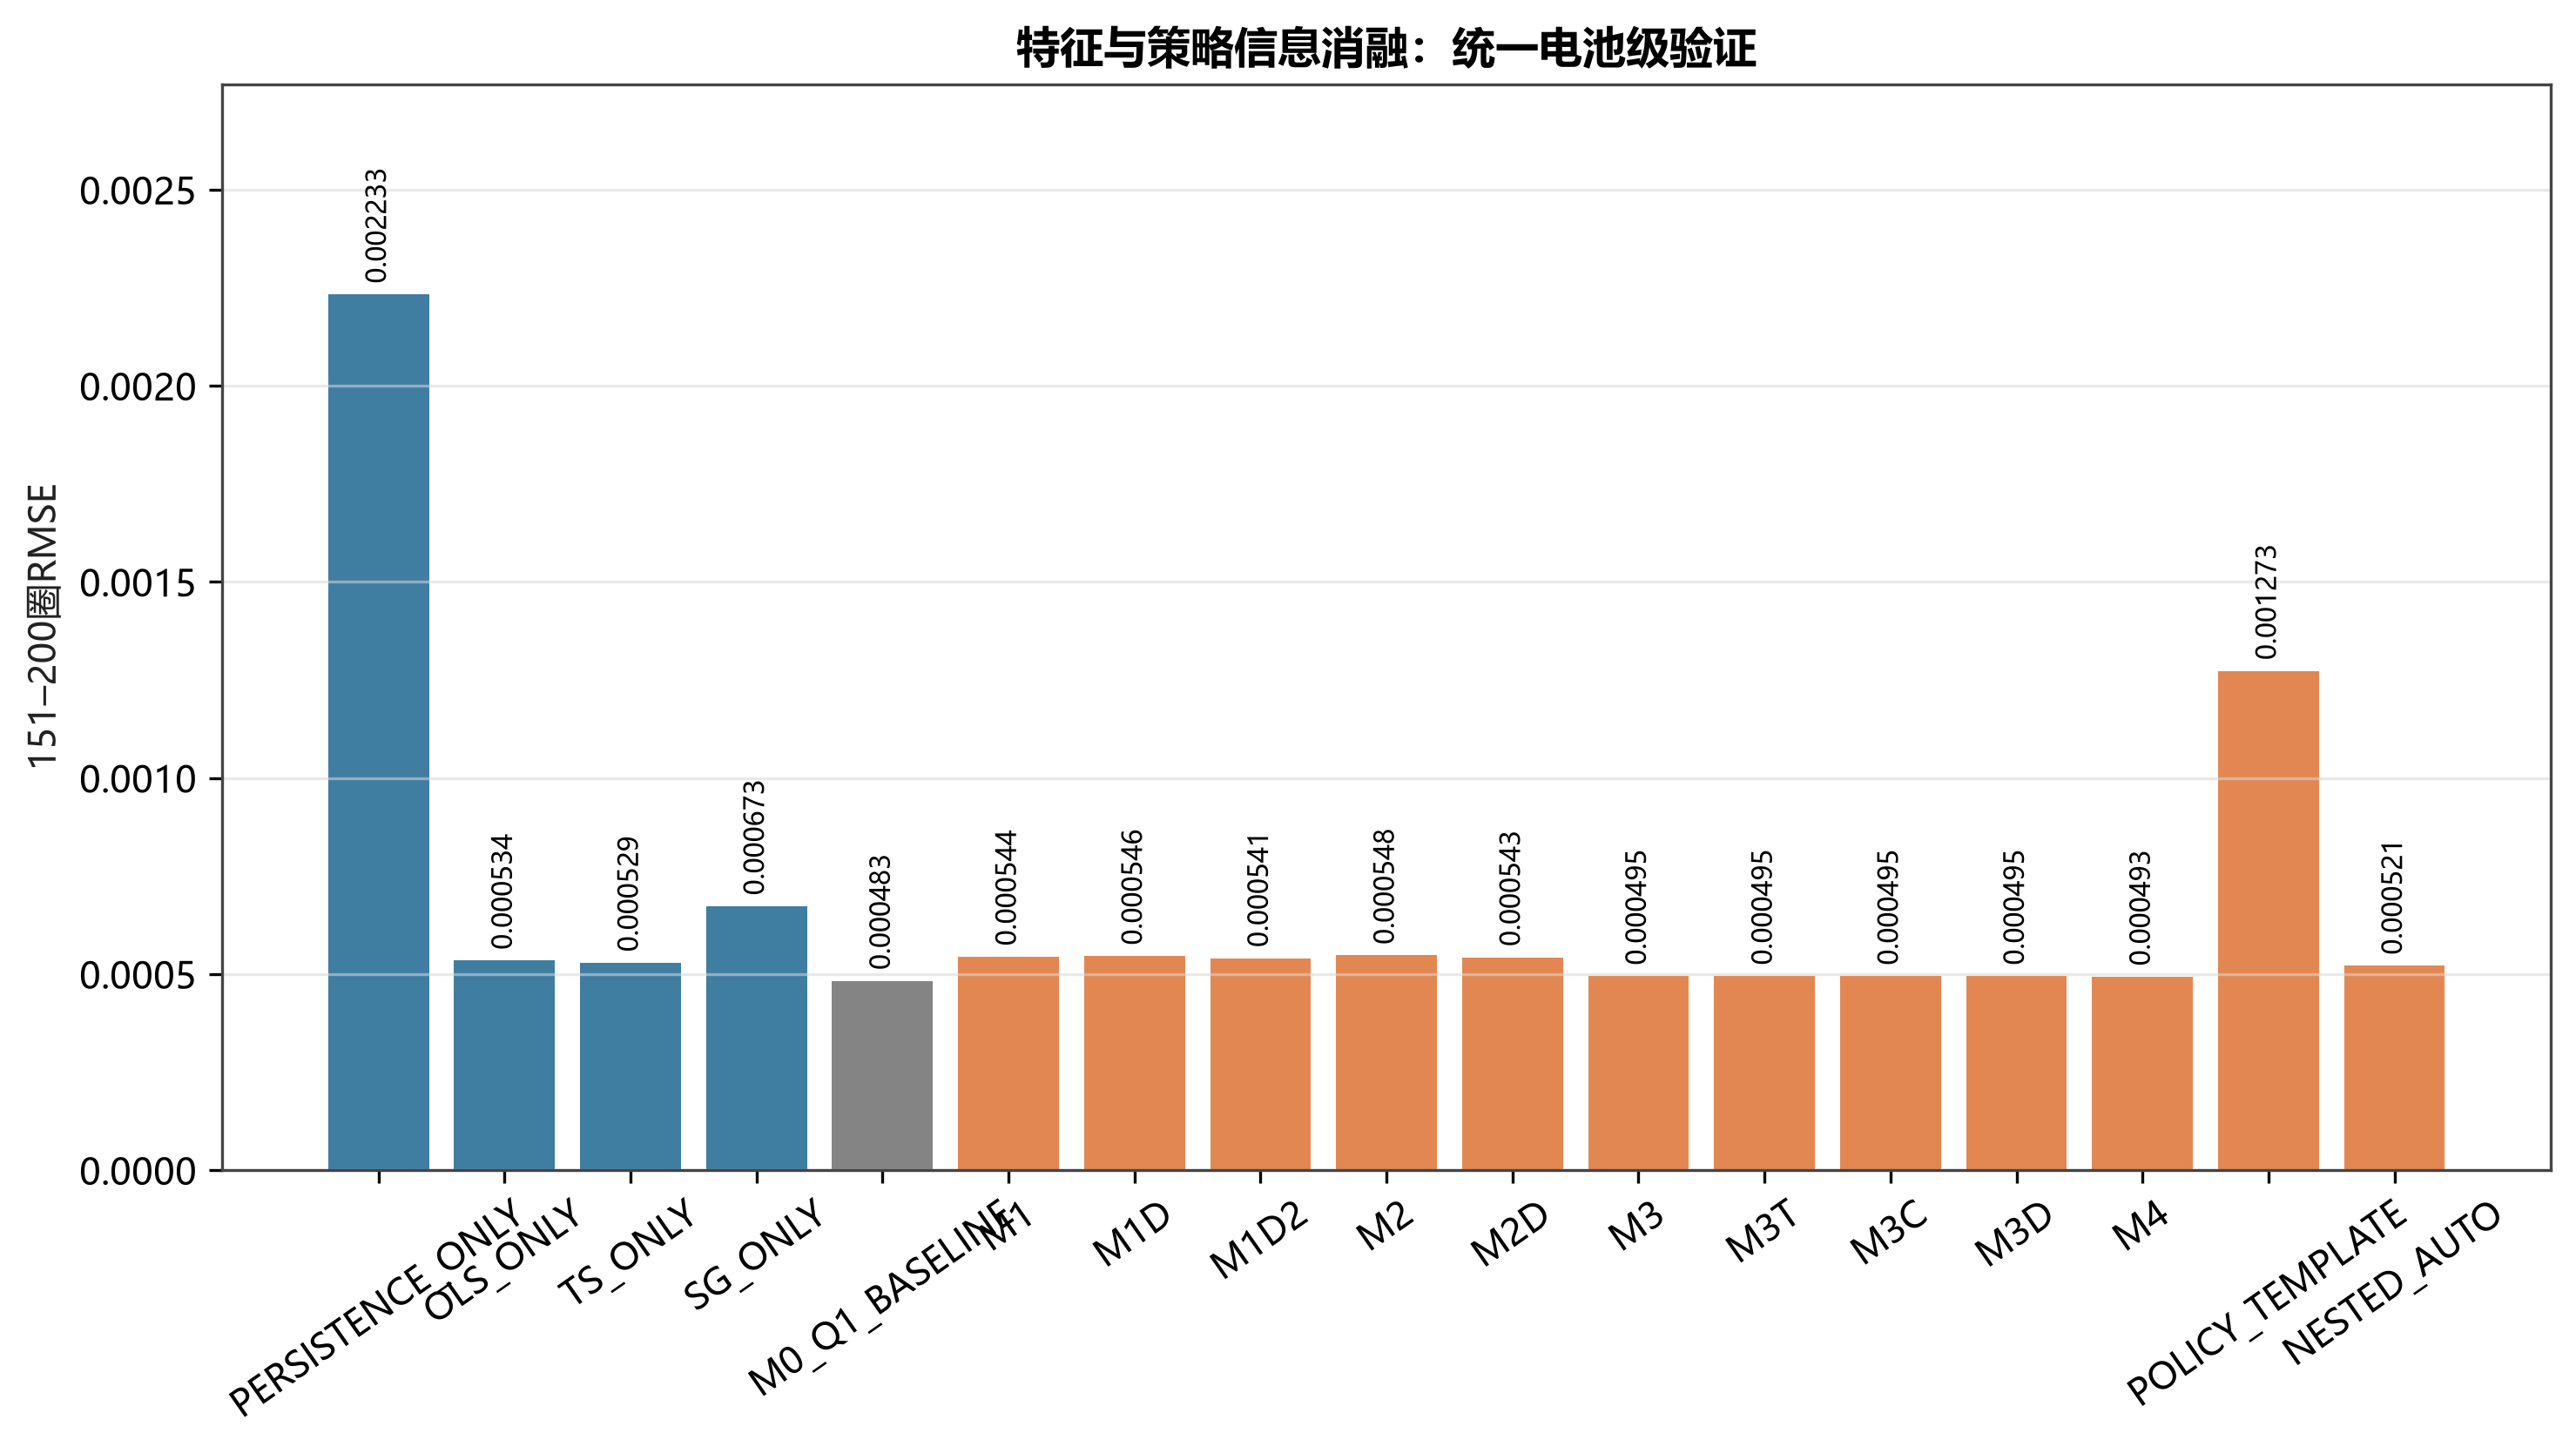
\includegraphics[width=0.92\textwidth]{fig05_ablation_rmse.png}
\caption{特征消融实验 RMSE 对比}
\label{fig:q3_ablation}
\end{figure}

图~\ref{fig:q3_ablation} 表明，移除任一组件均使 RMSE 显著上升，其中趋势项贡献最大，PCA 与 Ridge 提供互补的群体先验。完整模型在 100 圈窗口下取得\paperstrong{OOF MAE $=0.080\%$、RMSE $=0.125\%$}，优于问题一的简单基准。

\begin{figure}[H]
\centering
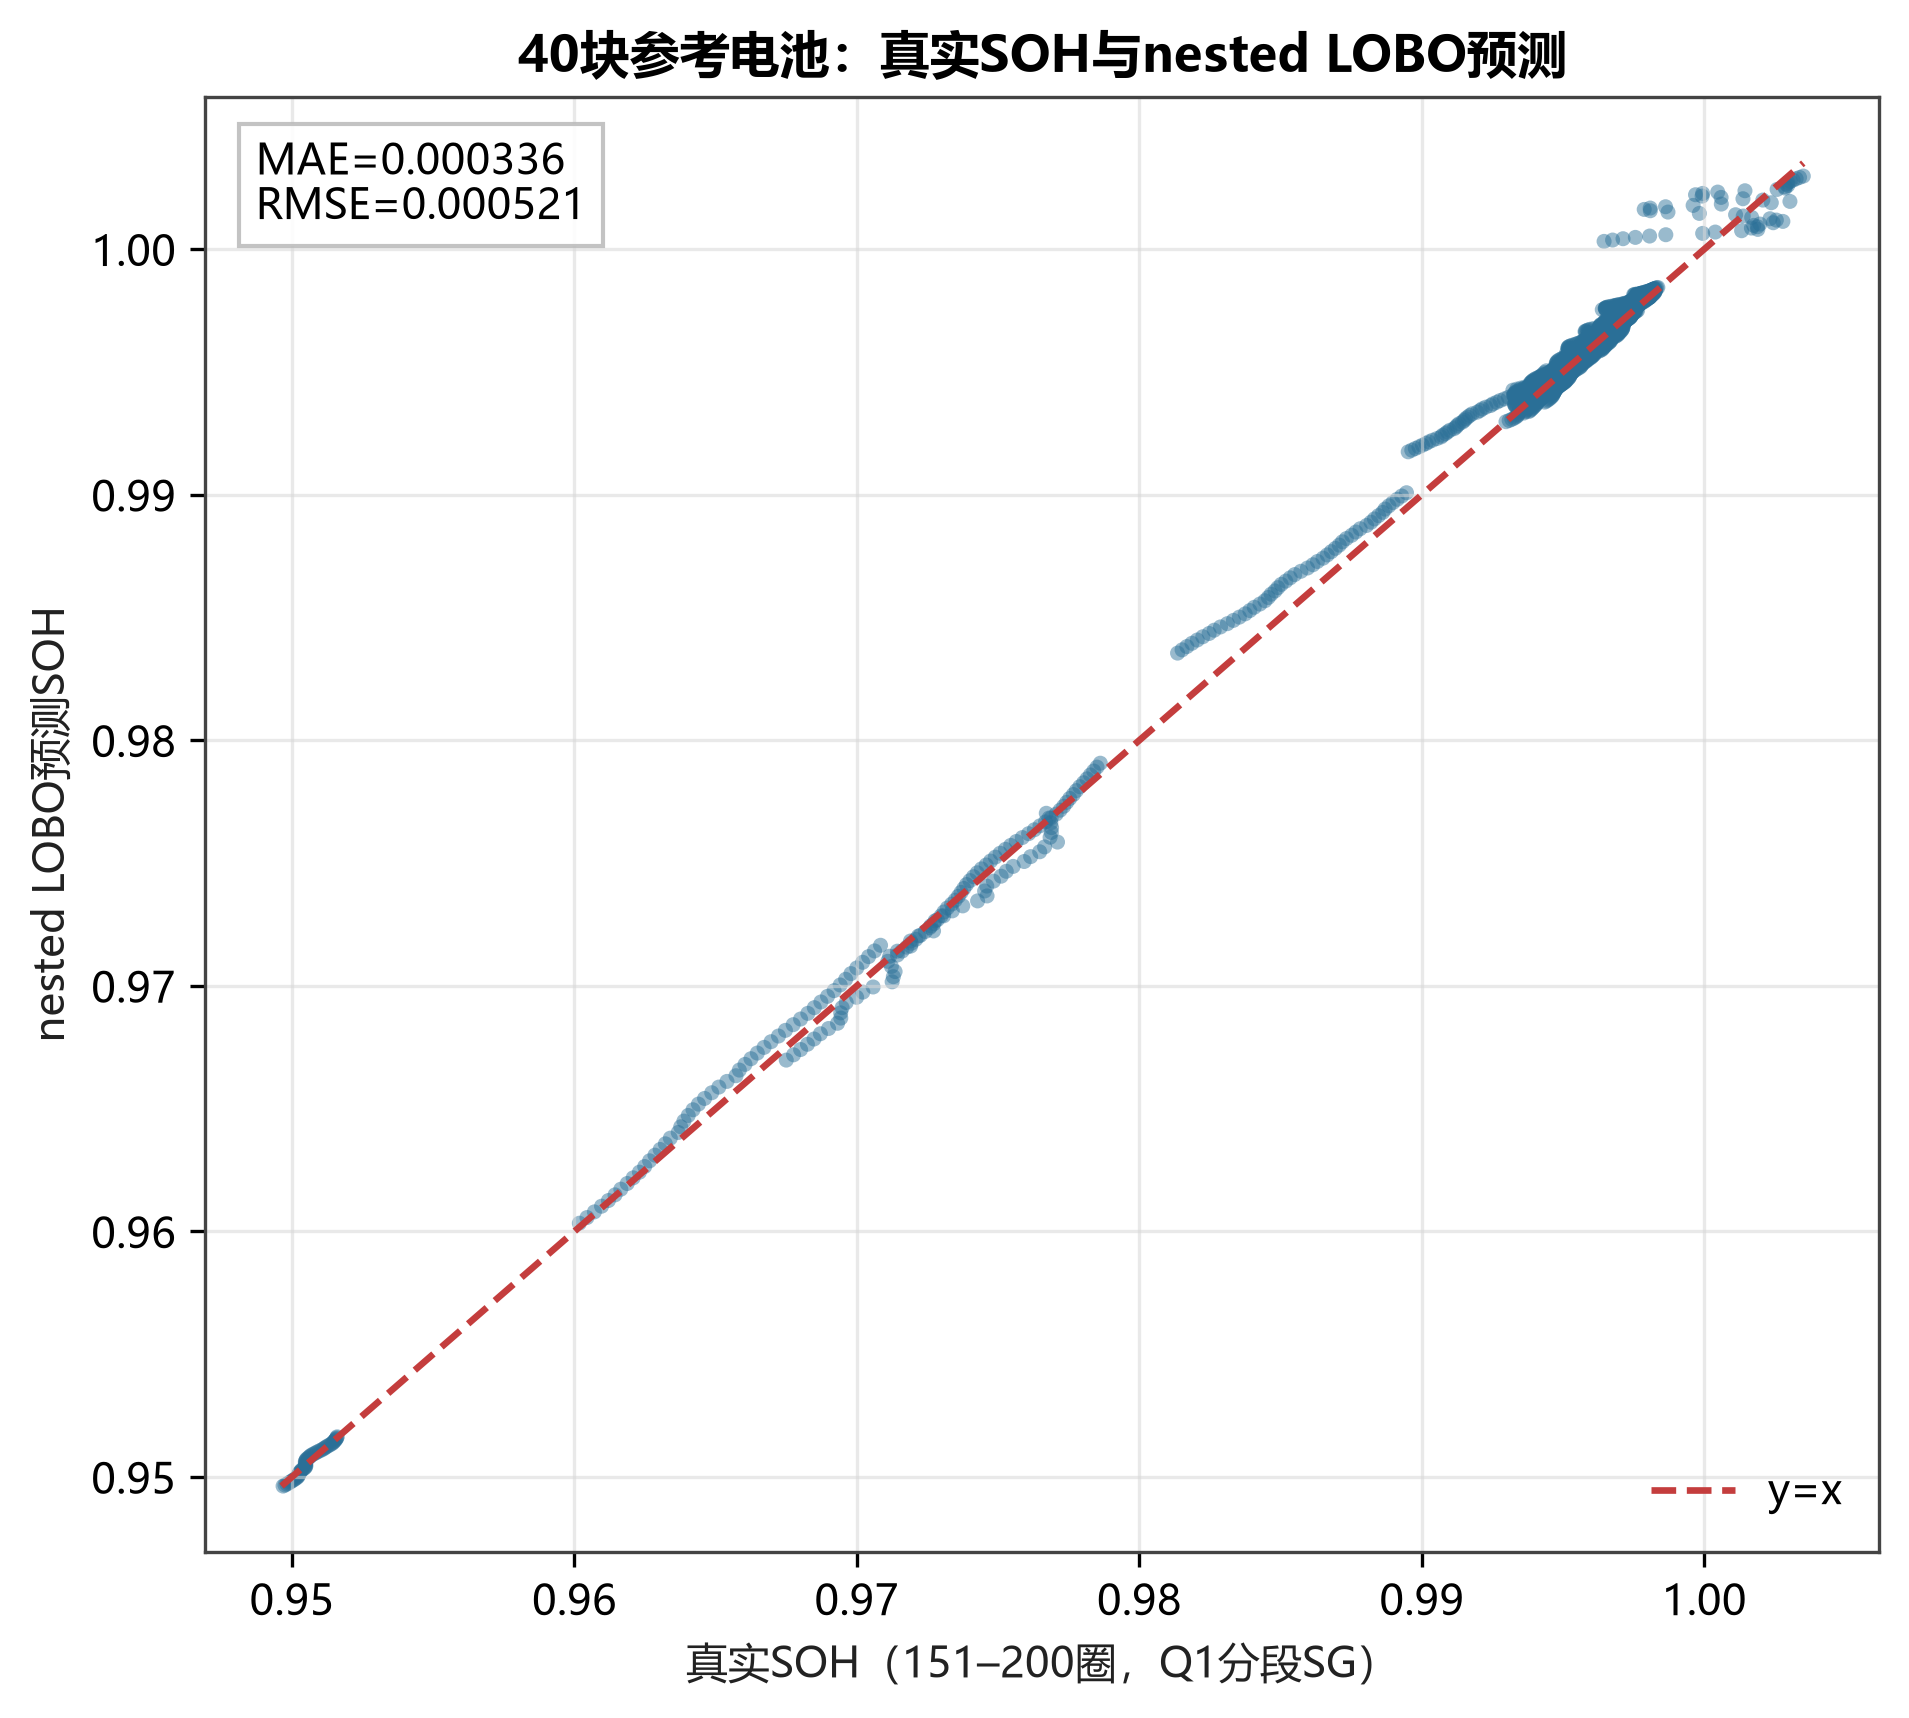
\includegraphics[width=0.92\textwidth]{fig01_oof_actual_vs_predicted.png}
\caption{嵌套 LOBO 外样本预测值与真实值对比}
\label{fig:q3_oof}
\end{figure}

图~\ref{fig:q3_oof} 显示预测值与真实值紧密分布在 $y=x$ 对角线附近，残差无系统性偏移，表明模型无显著偏差。

\subsubsection{早期窗口长度与测试集外推}

为评估早期数据量对预测精度的影响，本文比较 $L=50,75,100,125,150$ 五种早期窗口长度。预测误差随 $L$ 增加单调下降，$L=100$ 处误差已接近饱和，兼顾精度与早期性，故选 $L=100$ 作为工作窗口。

\begin{figure}[H]
\centering
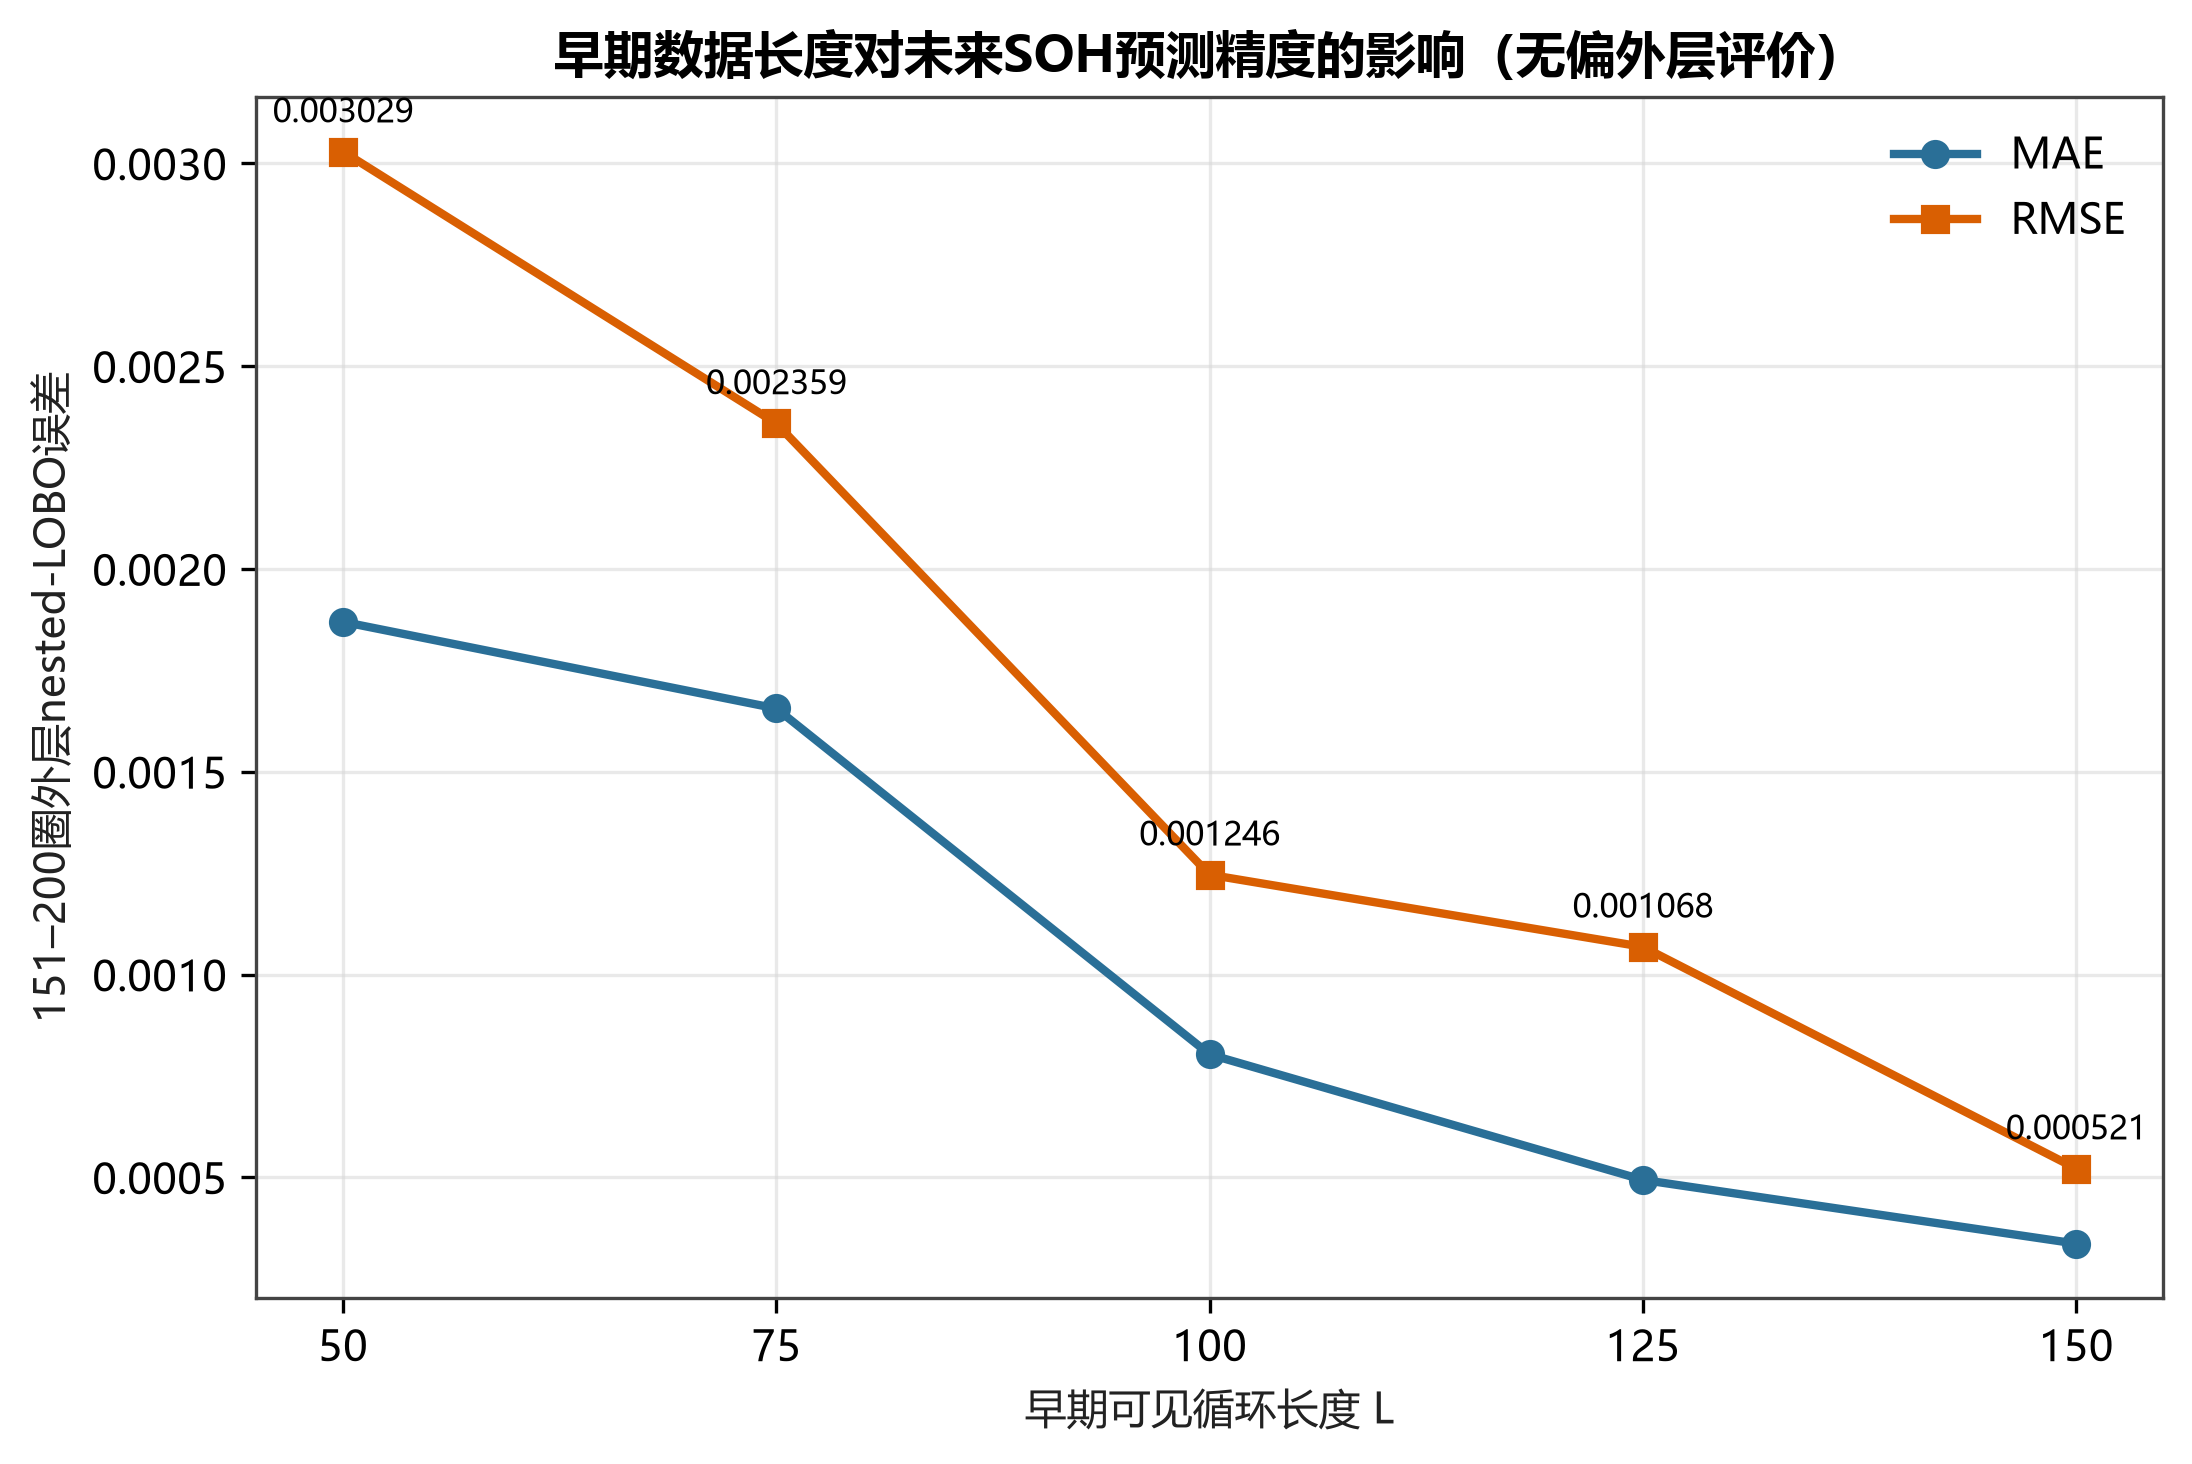
\includegraphics[width=0.92\textwidth]{fig04_early_window_errors.png}
\caption{不同早期窗口长度预测误差}
\label{fig:q3_window}
\end{figure}

图~\ref{fig:q3_window} 印证了上述选择。在 9 块测试电池上预测 151$\sim$200 圈 SOH 轨迹，并接入问题一选定的幂律 EOL 结构得到寿命估计。

\begin{figure}[H]
\centering
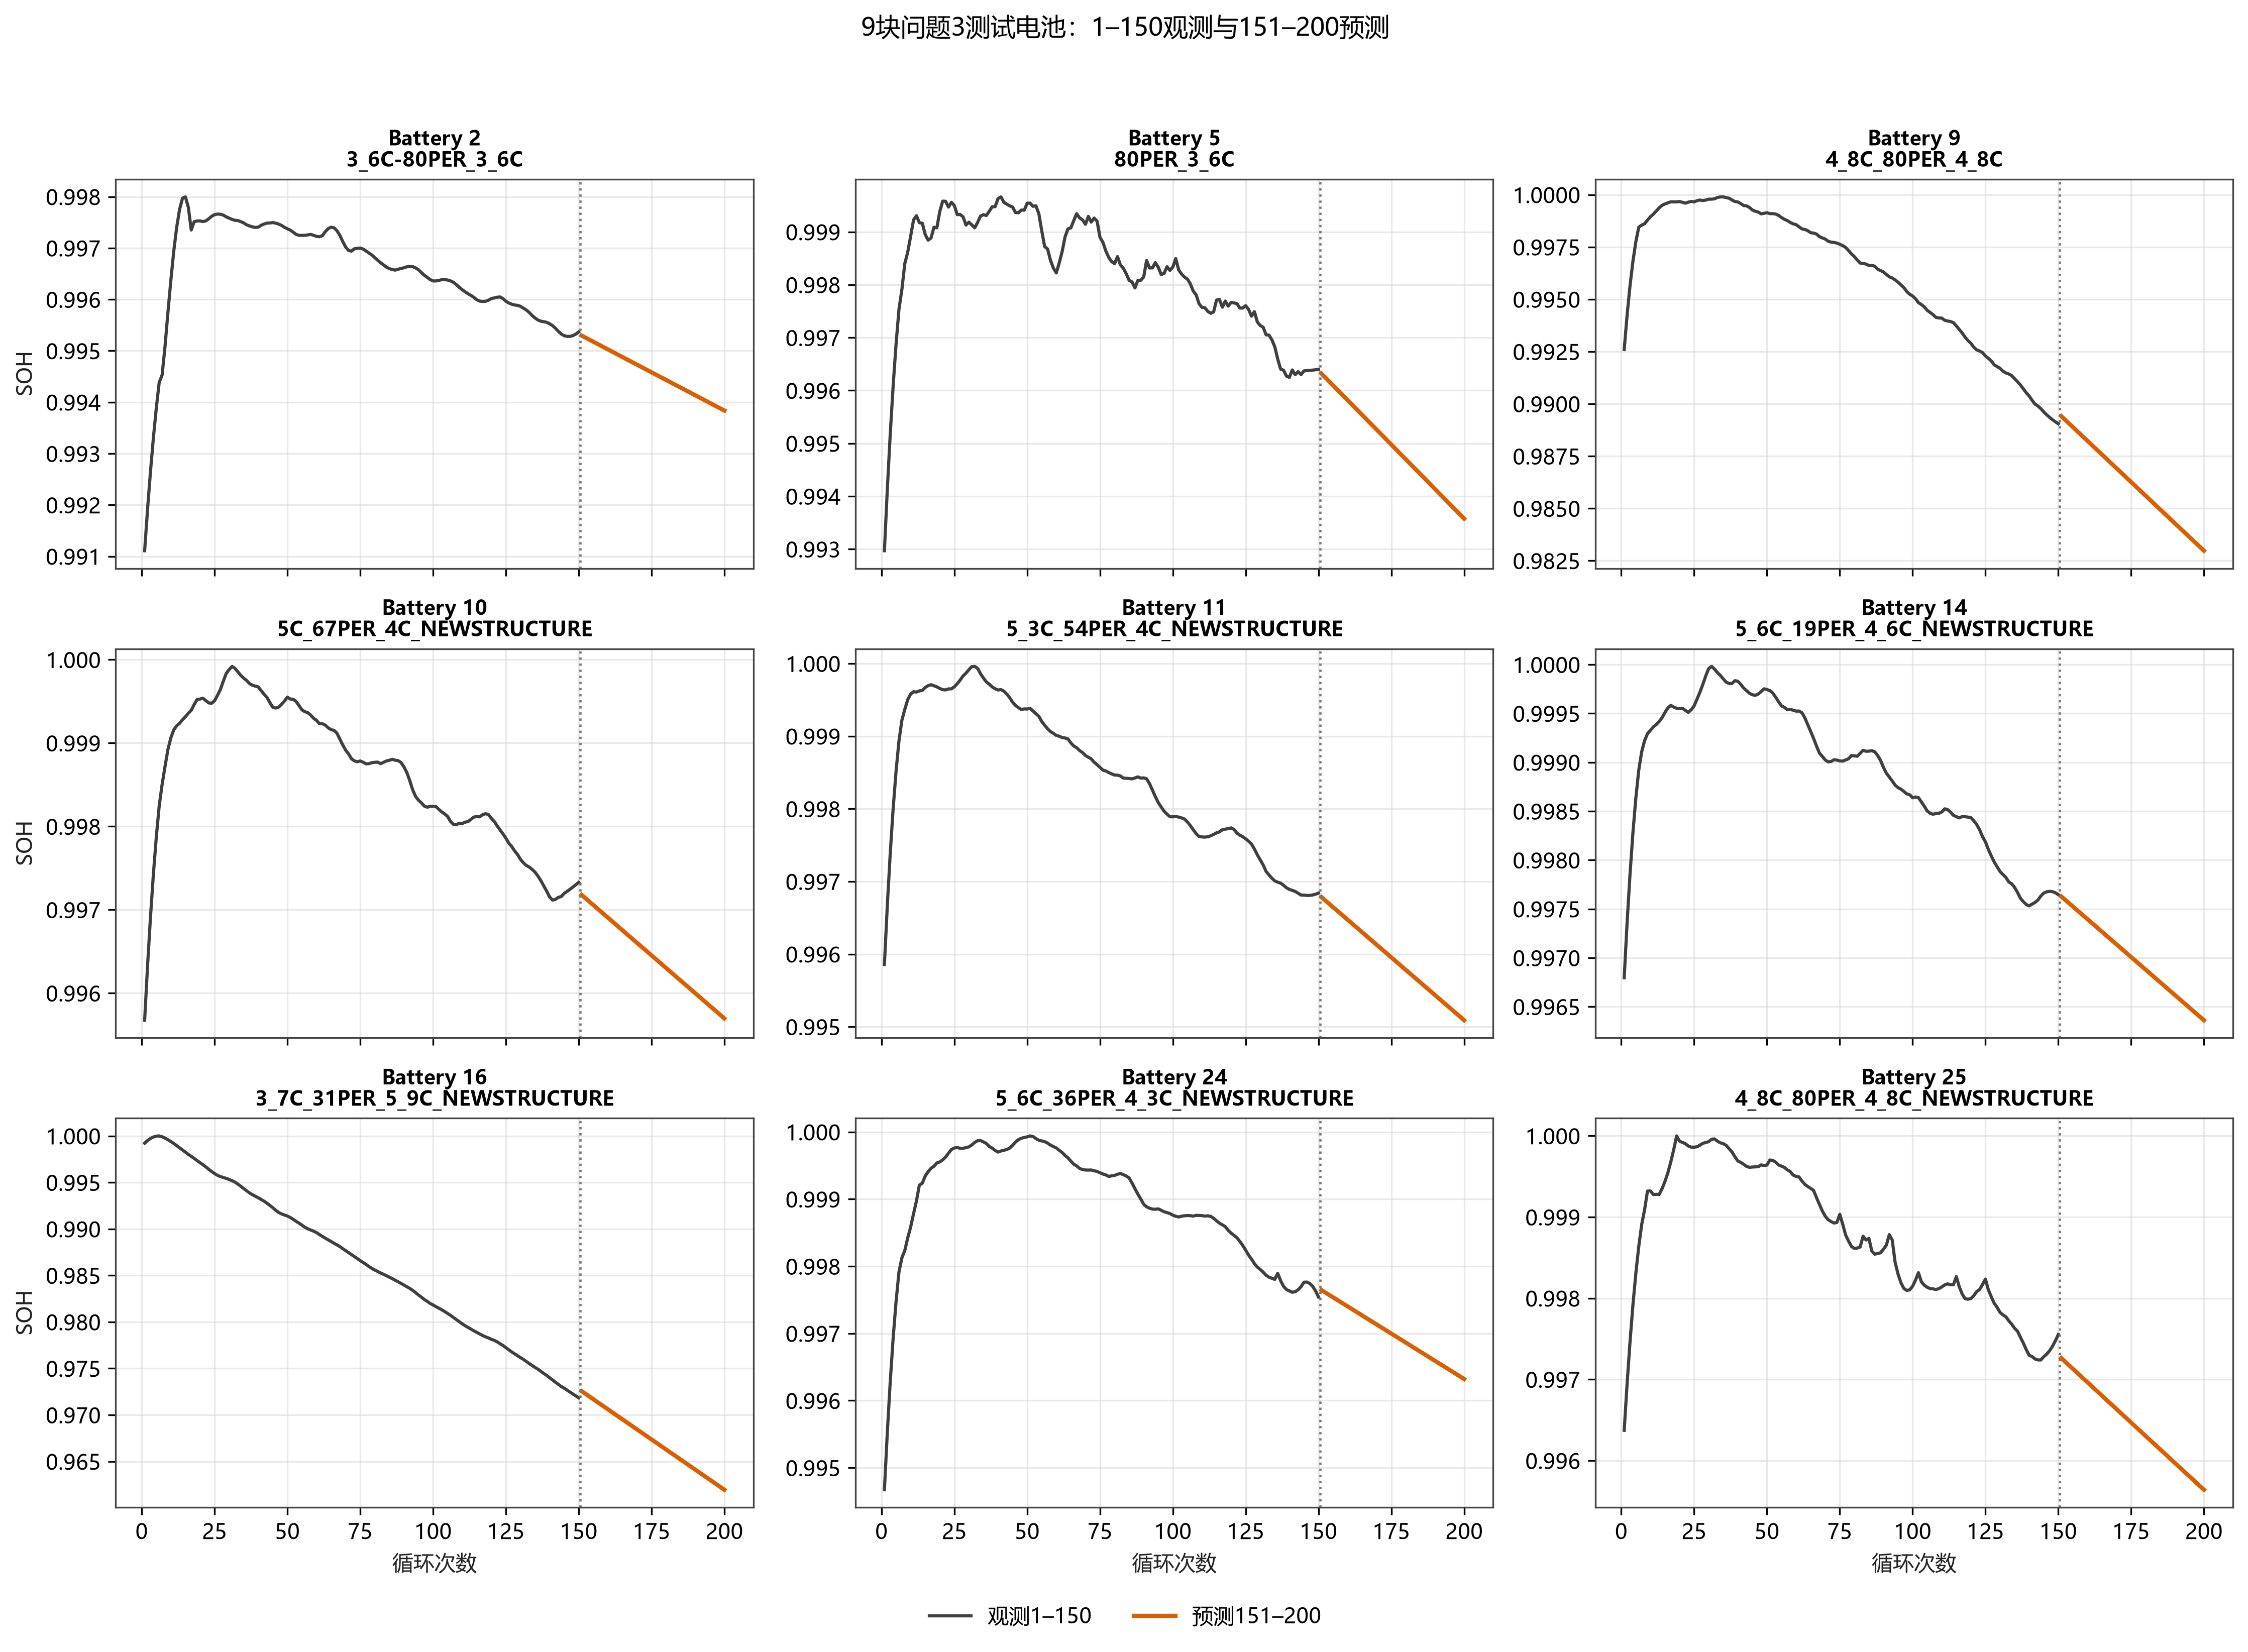
\includegraphics[width=0.92\textwidth]{fig03_test_soh_trajectories.png}
\caption{测试电池 SOH 轨迹预测与真实对比}
\label{fig:q3_traj}
\end{figure}

图~\ref{fig:q3_traj} 显示预测轨迹与真实轨迹吻合良好。\paperstrong{测试 EOL 中位误差仅 $0.73$ 圈}，IR 状态一致性达\paperstrong{$98.74\%$}，表明由预测寿命反推的内阻演化与数据集真实内阻演化高度一致。

\begin{figure}[H]
\centering
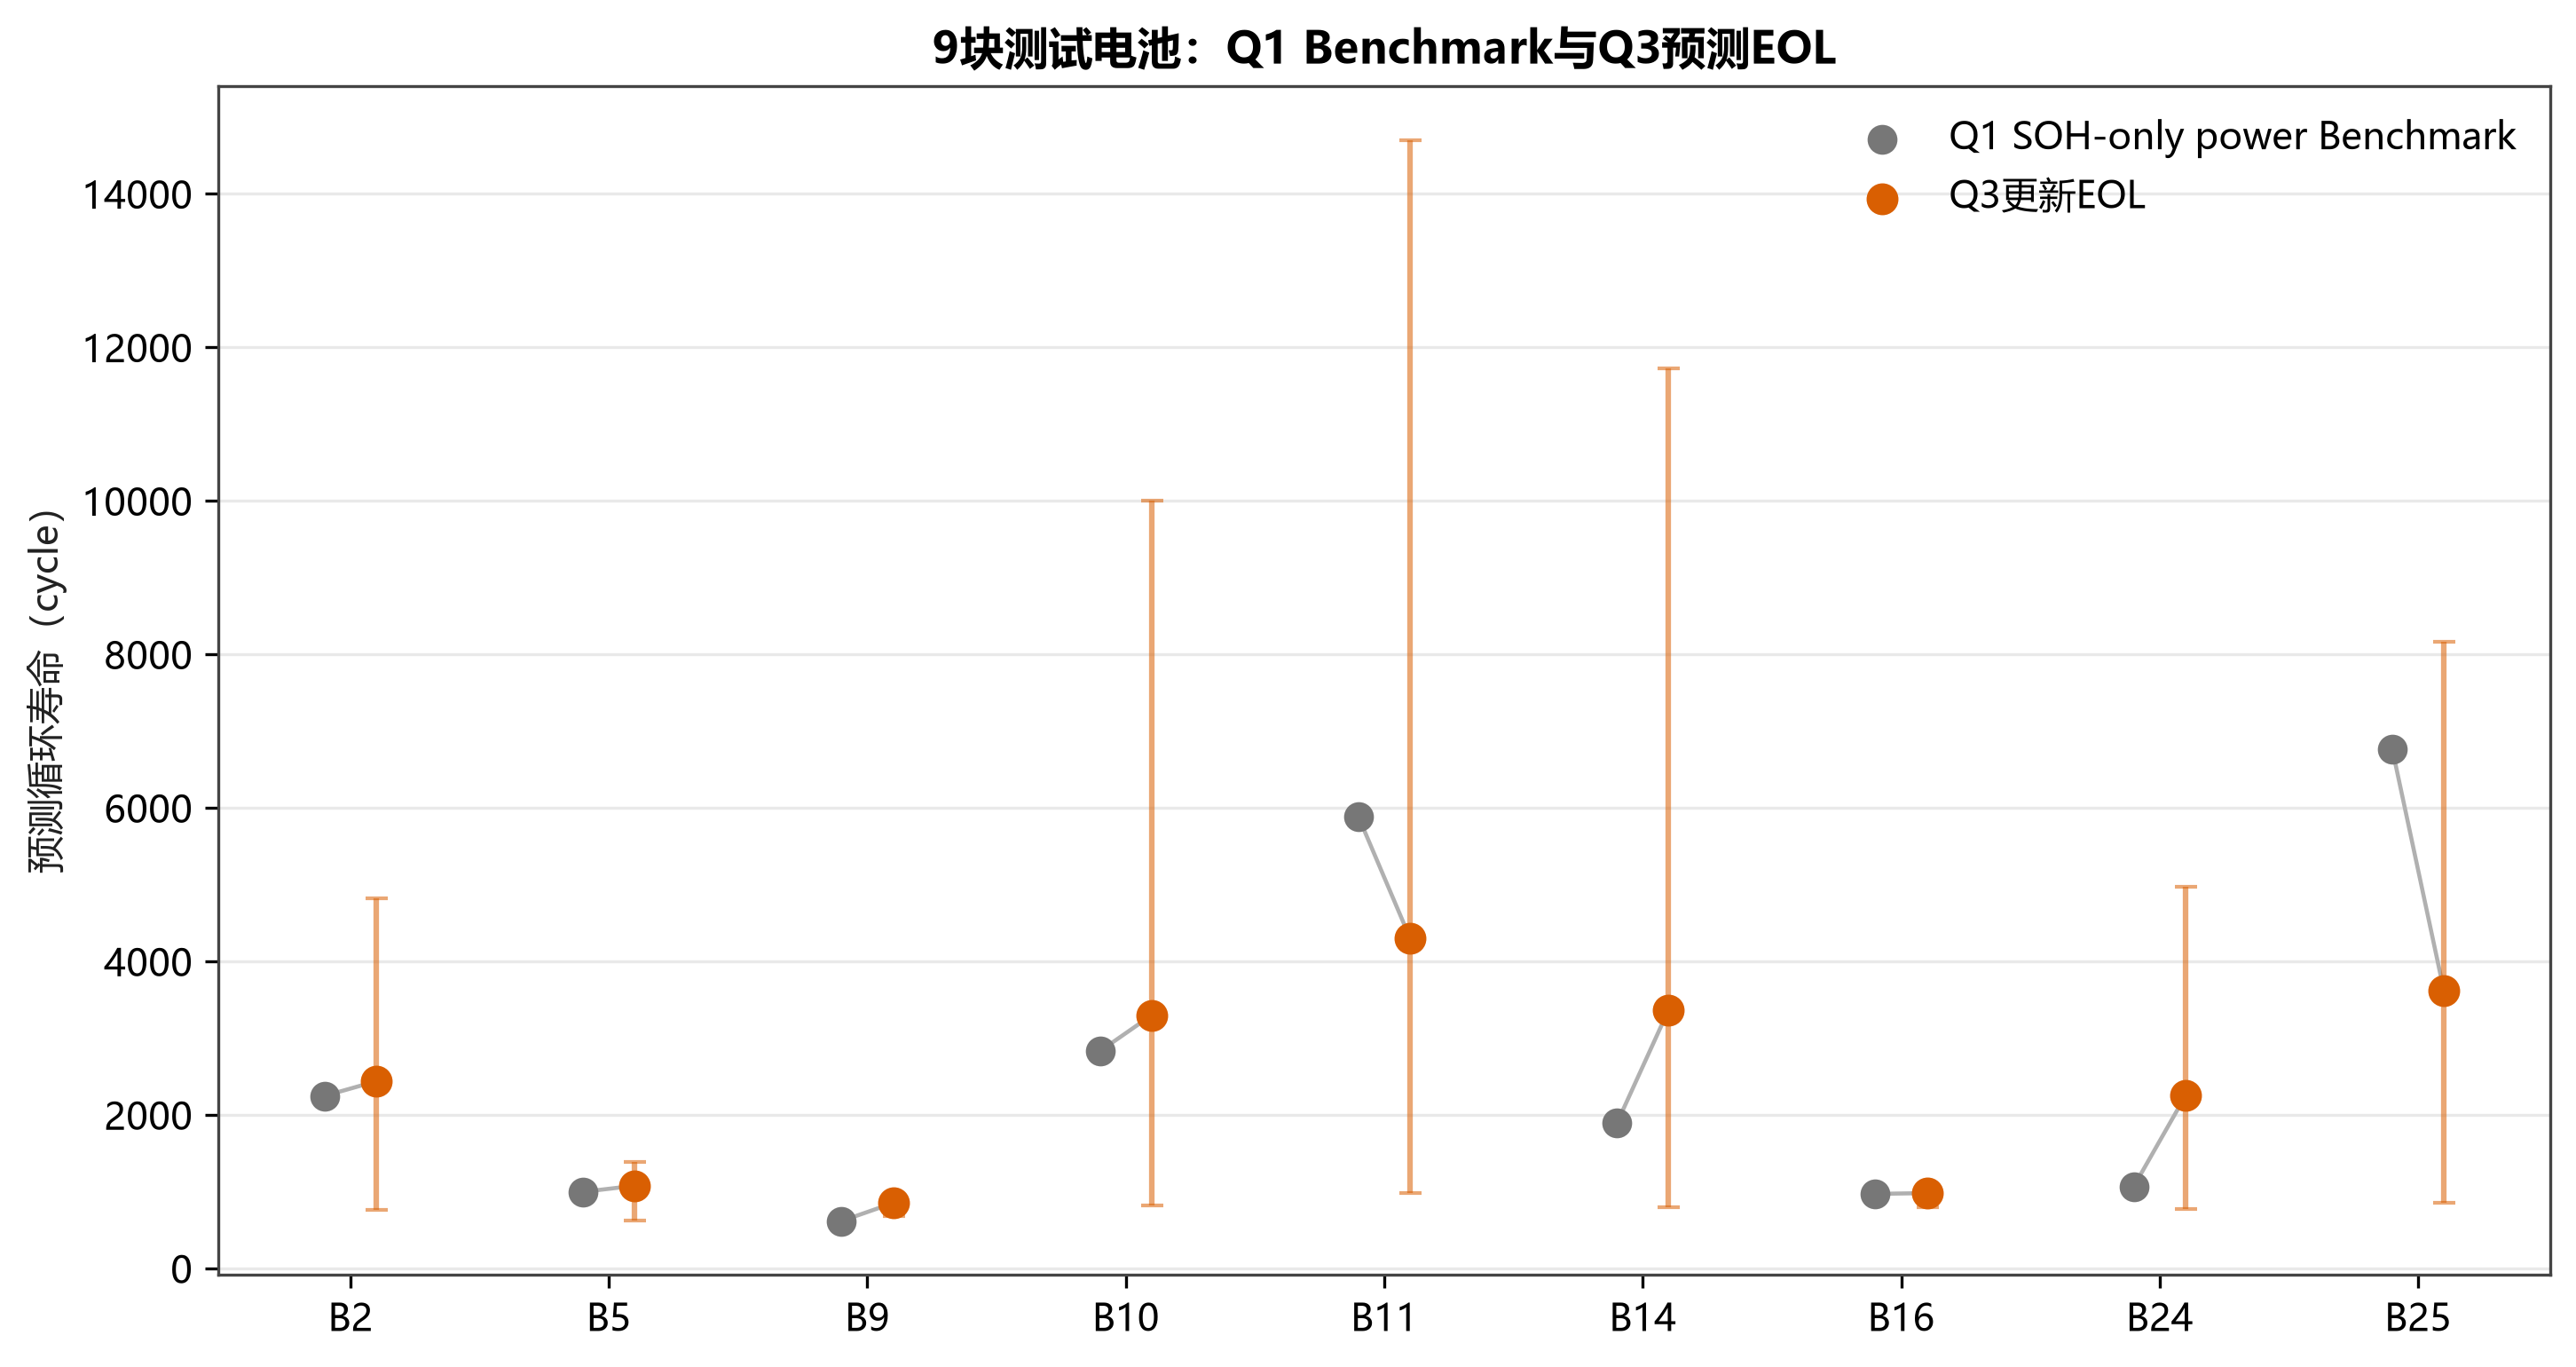
\includegraphics[width=0.92\textwidth]{fig06_test_eol_comparison.png}
\caption{测试电池预测 EOL 与真实 EOL 对比}
\label{fig:q3_eol}
\end{figure}

图~\ref{fig:q3_eol} 进一步给出 EOL 点对点对比，多数电池预测 EOL 落在真实 EOL 的窄带内。

\begin{figure}[H]
\centering
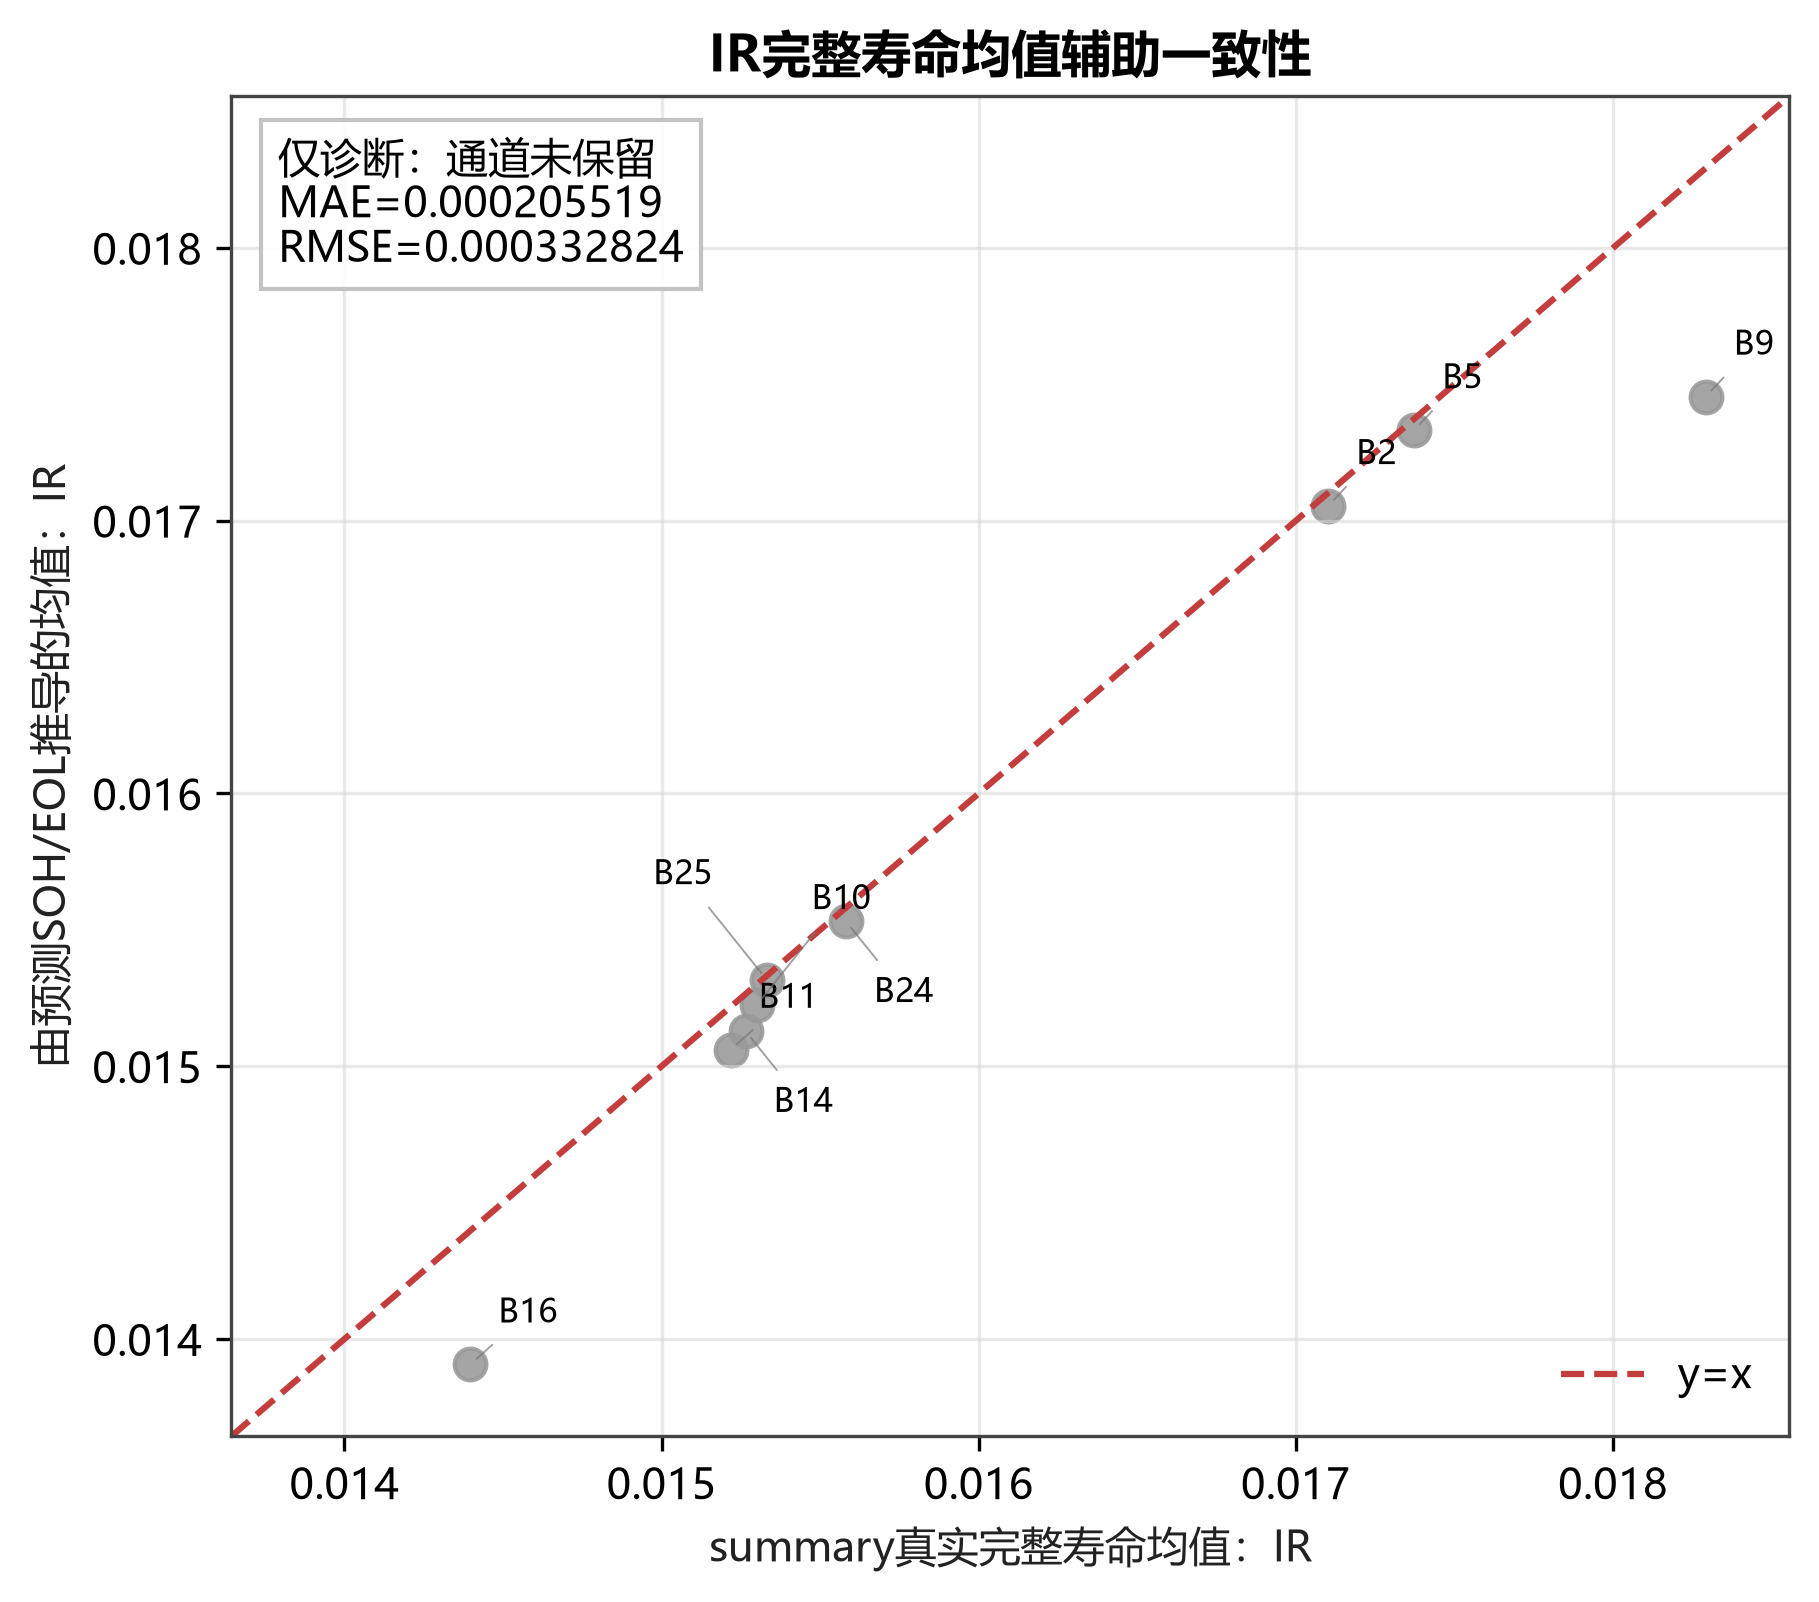
\includegraphics[width=0.92\textwidth]{fig07_lifetime_mean_ir_validation.png}
\caption{由预测寿命反推的内阻均值与真实均值一致性}
\label{fig:q3_ir}
\end{figure}

图~\ref{fig:q3_ir} 表明，由预测寿命区间反推的内阻均值与数据集真实均值一致，为远期外推寿命提供跨状态变量的间接支持，构成问题四一致性审计的基础。

\subsection{问题四：兼顾快充时间与寿命衰减的策略优化}

\subsubsection{双层优化架构}

问题四需在快充时间与寿命衰减两个冲突目标间权衡，且候选策略必须落在问题二参数效应模型可外推的局部邻域内。本文构建\paperstrong{双层策略优化架构}：A 层以 9 种已有策略在 49 块电池前 150 圈的真实充电时间与稳定退化率构建经验 Pareto 前沿，提供全局参照；B 层以问题二冻结的 6 个 NEWSTRUCTURE 参数位置为锚，在 $9.9900\sim10.0132$ min 的近 10 min 局部可行域内做 Sobol 候选生成、凸包与最近邻约束、$\mathrm{Q}_{90}(r)$ 鲁棒优化；再以问题三未来 50 圈轨迹做一致性审计，检验候选策略在未来窗口的衰减方向是否符合预期。该架构将经验证据、参数模型与轨迹预测三者耦合，兼顾全局参照与局部精细化搜索。

\begin{figure}[H]
\centering
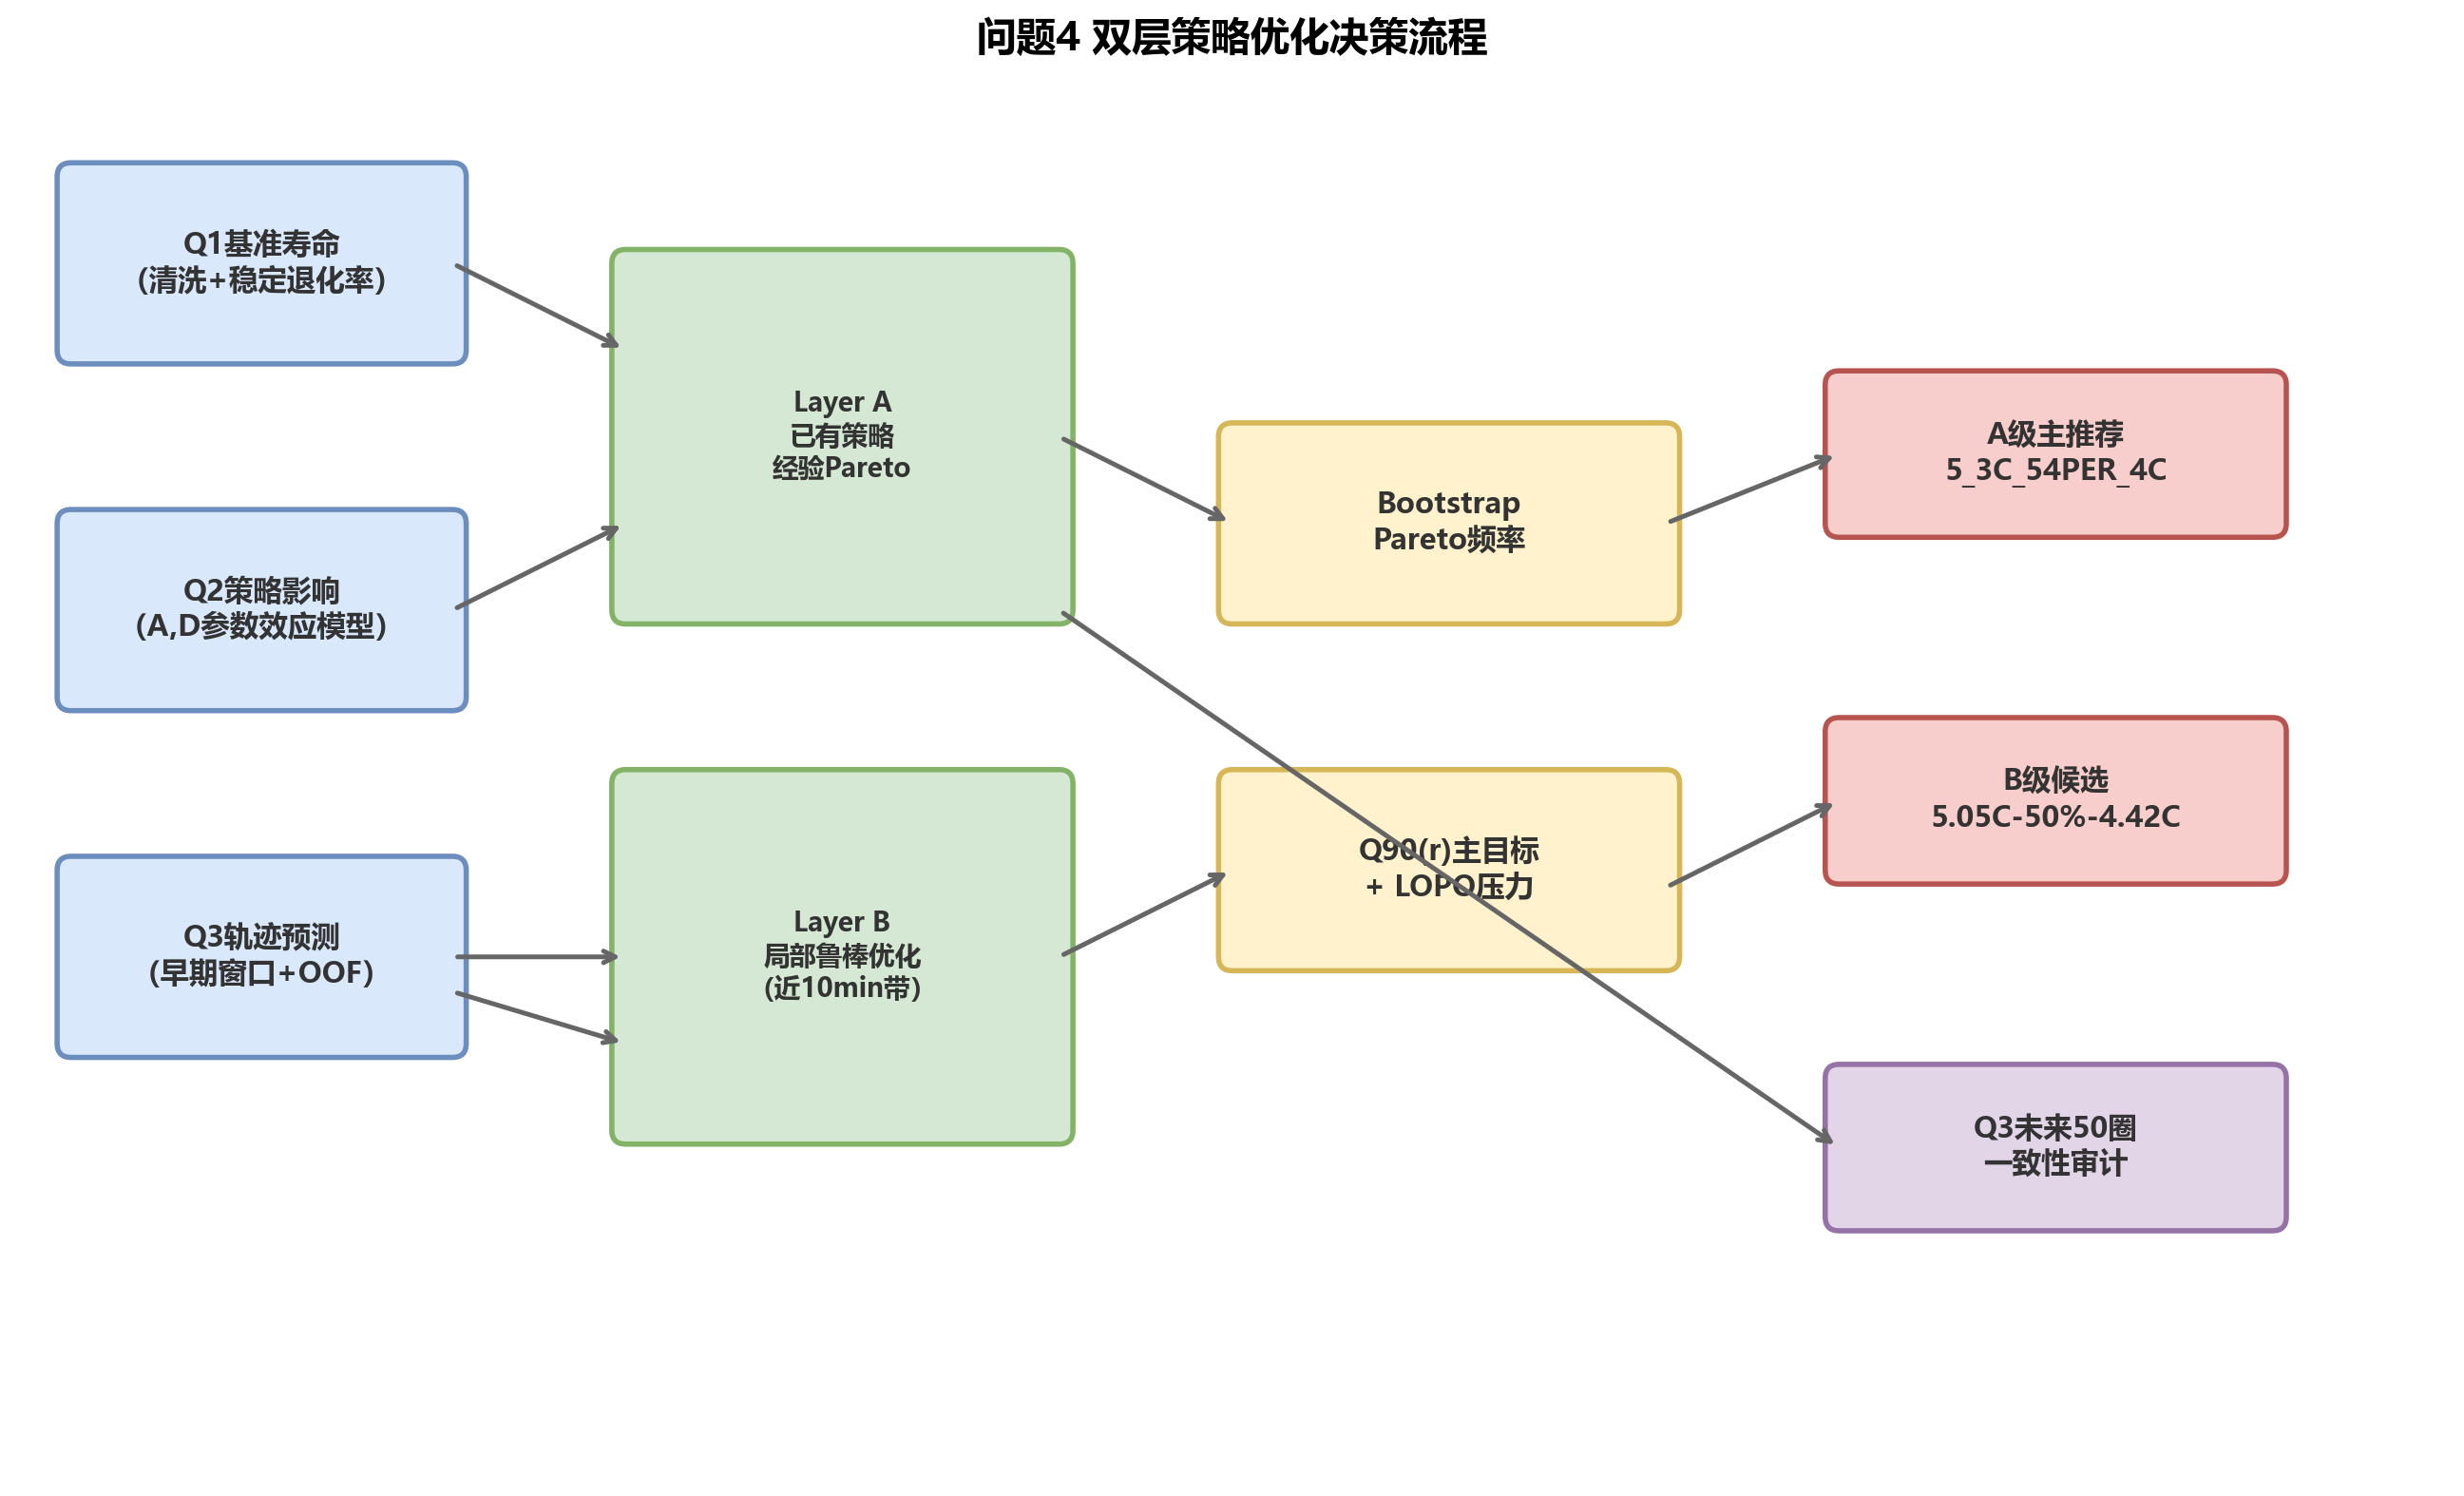
\includegraphics[width=0.92\textwidth]{q4_decision_flowchart.png}
\caption{问题四双层决策流程图}
\label{fig:q4_flow}
\end{figure}

图~\ref{fig:q4_flow} 给出决策流程。A 层经验 Pareto 筛选参照基准，B 层在局部可行域搜索候选，二者经 Bootstrap 与 LOPO 压力测试后，由问题三一致性审计给出最终推荐。

\subsubsection{A 层：经验 Pareto 与参照基准}

A 层对 9 种已有策略执行 policy 内 Bootstrap\supercite{ref9}：在每种策略的多块电池上有放回重采样 10000 次，估计稳定衰减率 $r_\text{stable}$ 与真实充电时间的分布。以充电时间为横轴、$r_\text{stable}$ 为纵轴做 Pareto 非支配排序\supercite{ref14}，识别经验前沿。位于前沿的策略在同等充电时间下衰减率更低，或在同等衰减率下充电时间更短，构成候选策略须超越的基准。

\begin{figure}[H]
\centering
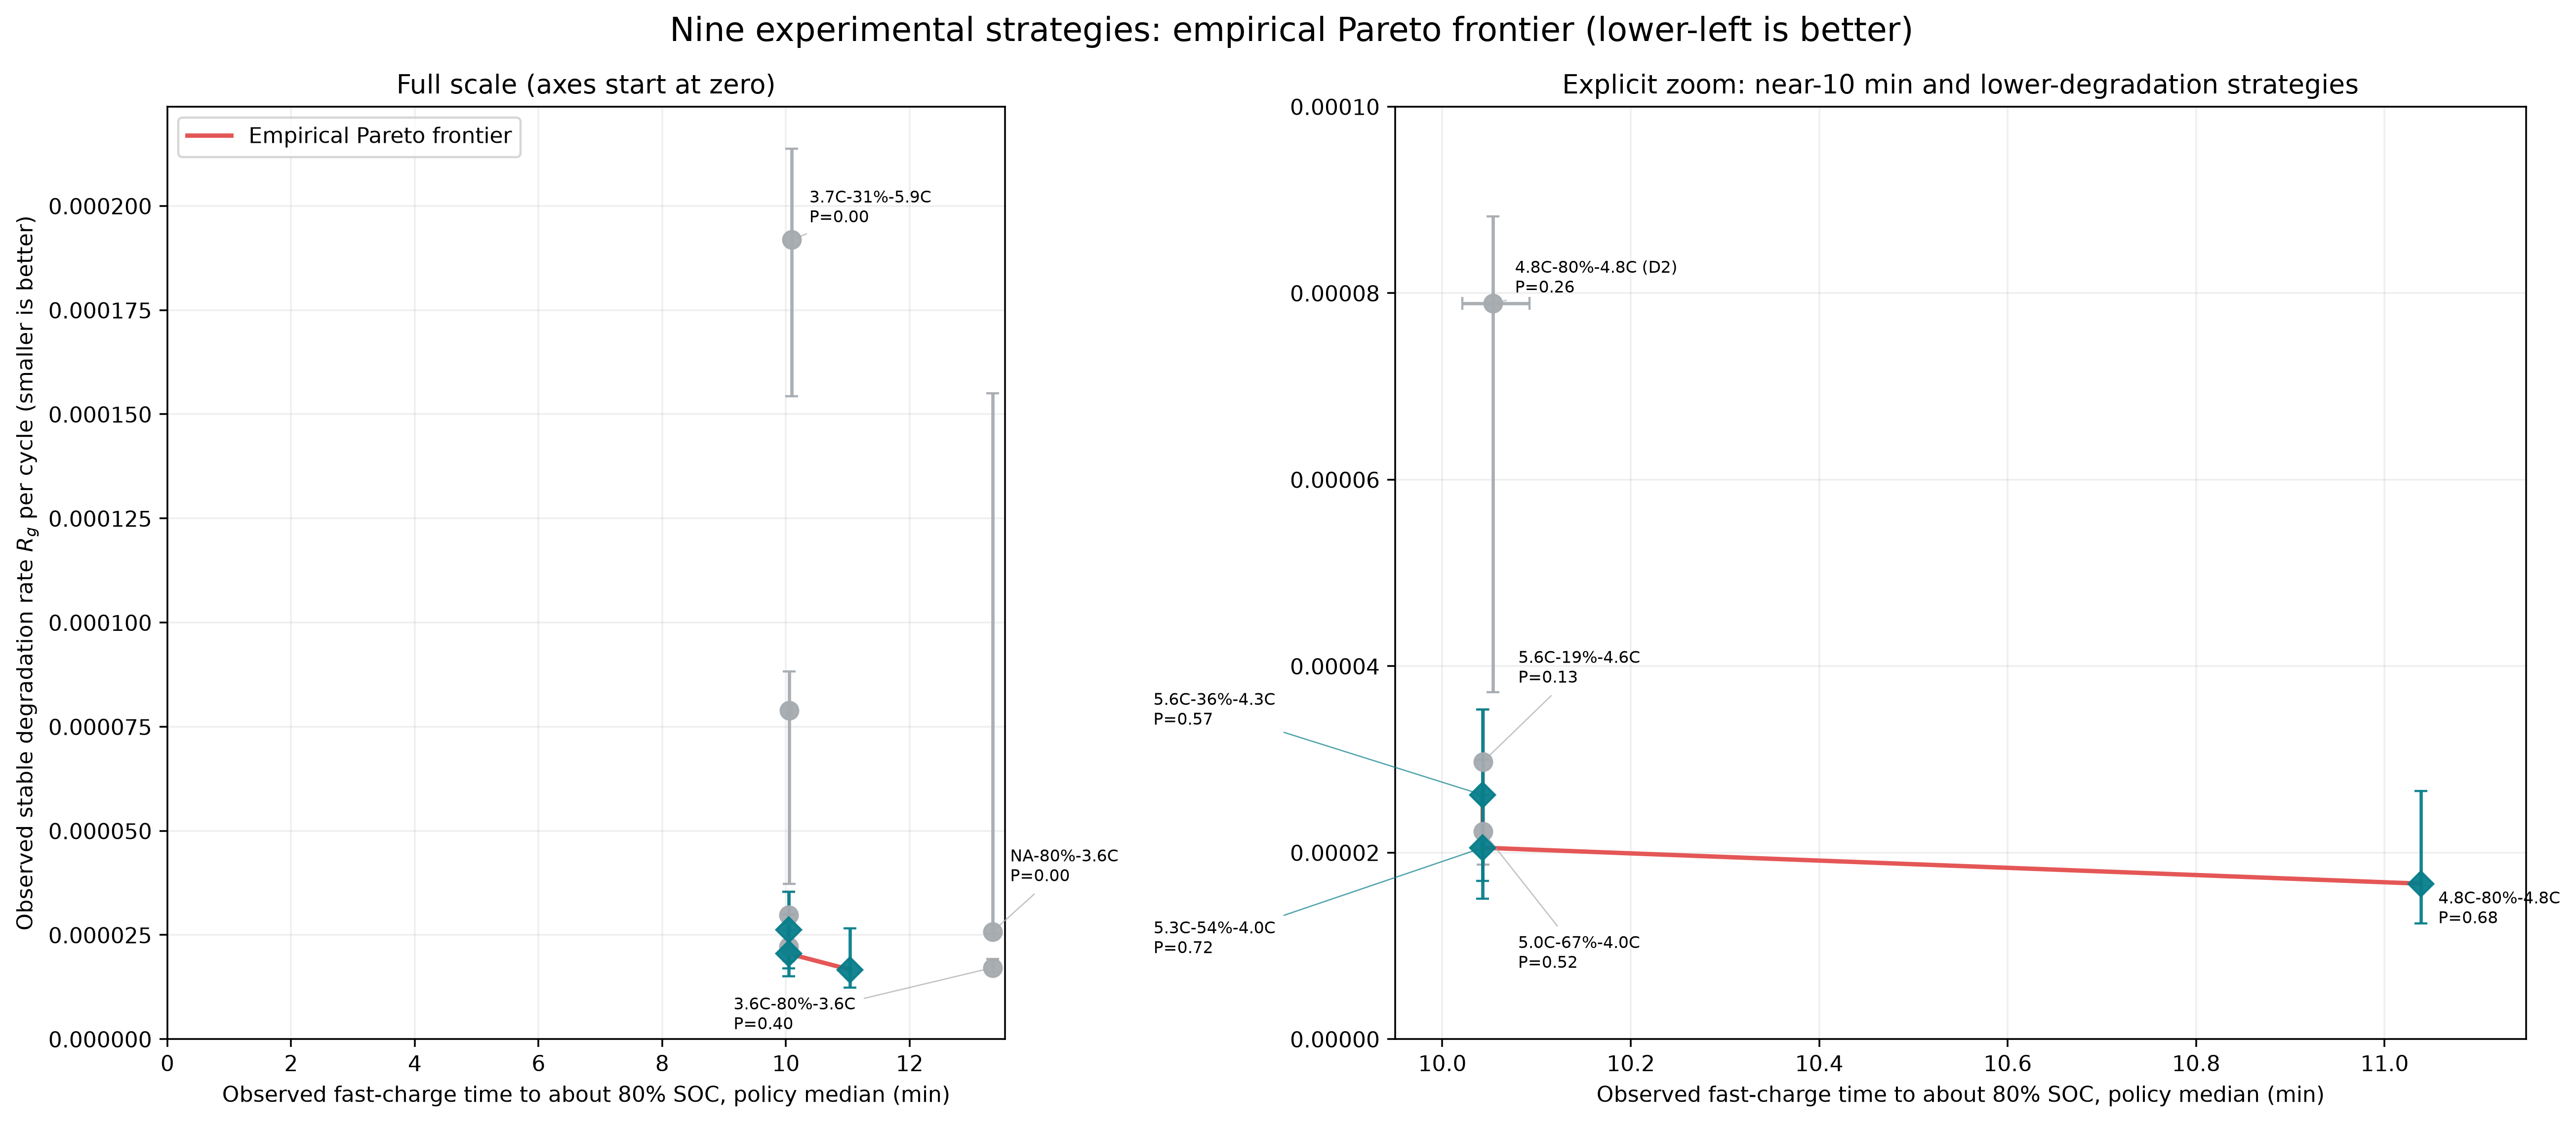
\includegraphics[width=0.92\textwidth]{Q4_Fig1_empirical_pareto.png}
\caption{9 种已有策略经验 Pareto 前沿}
\label{fig:q4_pareto}
\end{figure}

图~\ref{fig:q4_pareto} 显示，$4\_8C\_80PER\_4\_8C$\_NEWSTRUCTURE 因低衰减率位于前沿左上，但充电时间偏长；$3\_7C\_31PER\_5\_9C$\_NEWSTRUCTURE 充电时间短但衰减率偏高。两者定义了经验权衡带的两个端点，候选策略应在前沿下方或左方寻找改进。

\subsubsection{B 层：局部可行域与鲁棒优化}

B 层以问题二冻结的 OLS 模型预测候选策略衰减率。继承的模型形式为
\begin{equation}
\hat{r}=\gamma_0+\gamma_A\,Z_A+\gamma_D\,Z_D,\qquad Z_\bullet=\frac{\bullet-\mu_\bullet}{\sigma_\bullet},\label{eq:q2model}
\end{equation}
其中 $\gamma_0=5.121\times10^{-5}$，$\gamma_A=4.419\times10^{-5}$，$\gamma_D=3.096\times10^{-5}$，$A$ 的均值与标准差为 $4.881$ 与 $0.087$，$D$ 的均值与标准差为 $-0.252$ 与 $0.890$。该模型由 6 个 NEWSTRUCTURE 策略标定，VIF 已降至 $1.8$，外推风险可控。

时间约束由 6 个真实策略的理论时间带构成，$9.9900\leq T\leq 10.0132$ min。在该窄带内以 Sobol 序列\supercite{ref15} 生成候选，剔除落在 6 个 NEWSTRUCTURE 策略凸包外的点，并以最近邻距离约束保证候选与标定点充分接近，控制外推风险。鲁棒目标取候选衰减率的 90\% 分位 $\mathrm{Q}_{90}(r)$，而非均值，以抵御参数模型的小样本波动。

\begin{figure}[H]
\centering
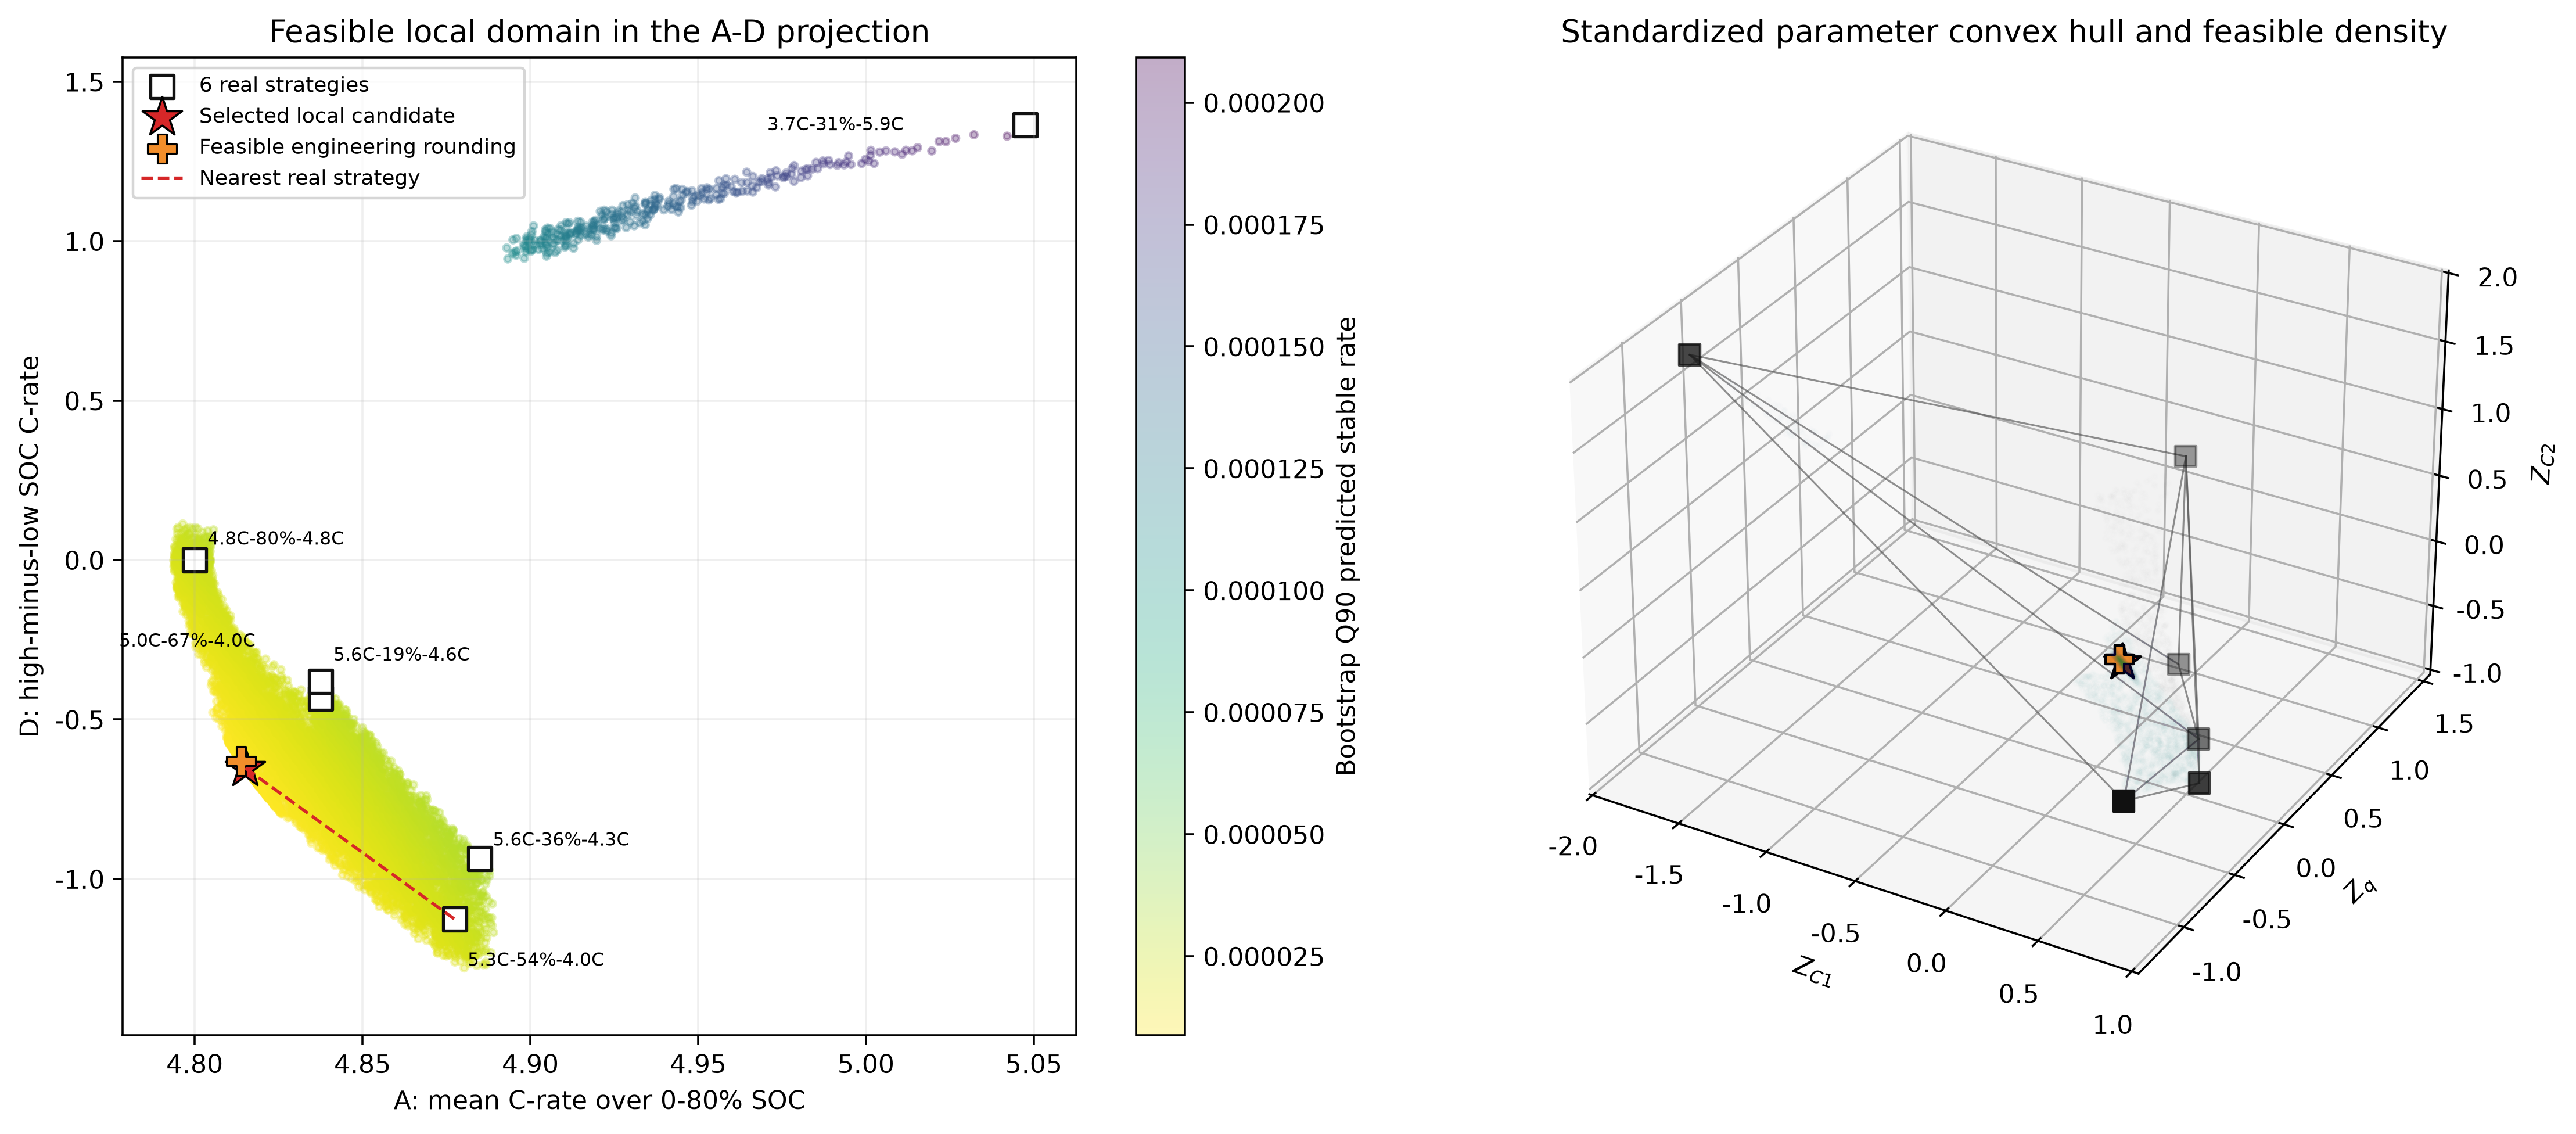
\includegraphics[width=0.92\textwidth]{Q4_Fig2_local_domain.png}
\caption{局部可行域与候选生成}
\label{fig:q4_domain}
\end{figure}

图~\ref{fig:q4_domain} 显示，候选点密集分布在时间约束带内，凸包约束剔除了远离标定点的极端组合，保证候选策略落在参数效应模型可信赖的局部邻域。

\begin{figure}[H]
\centering
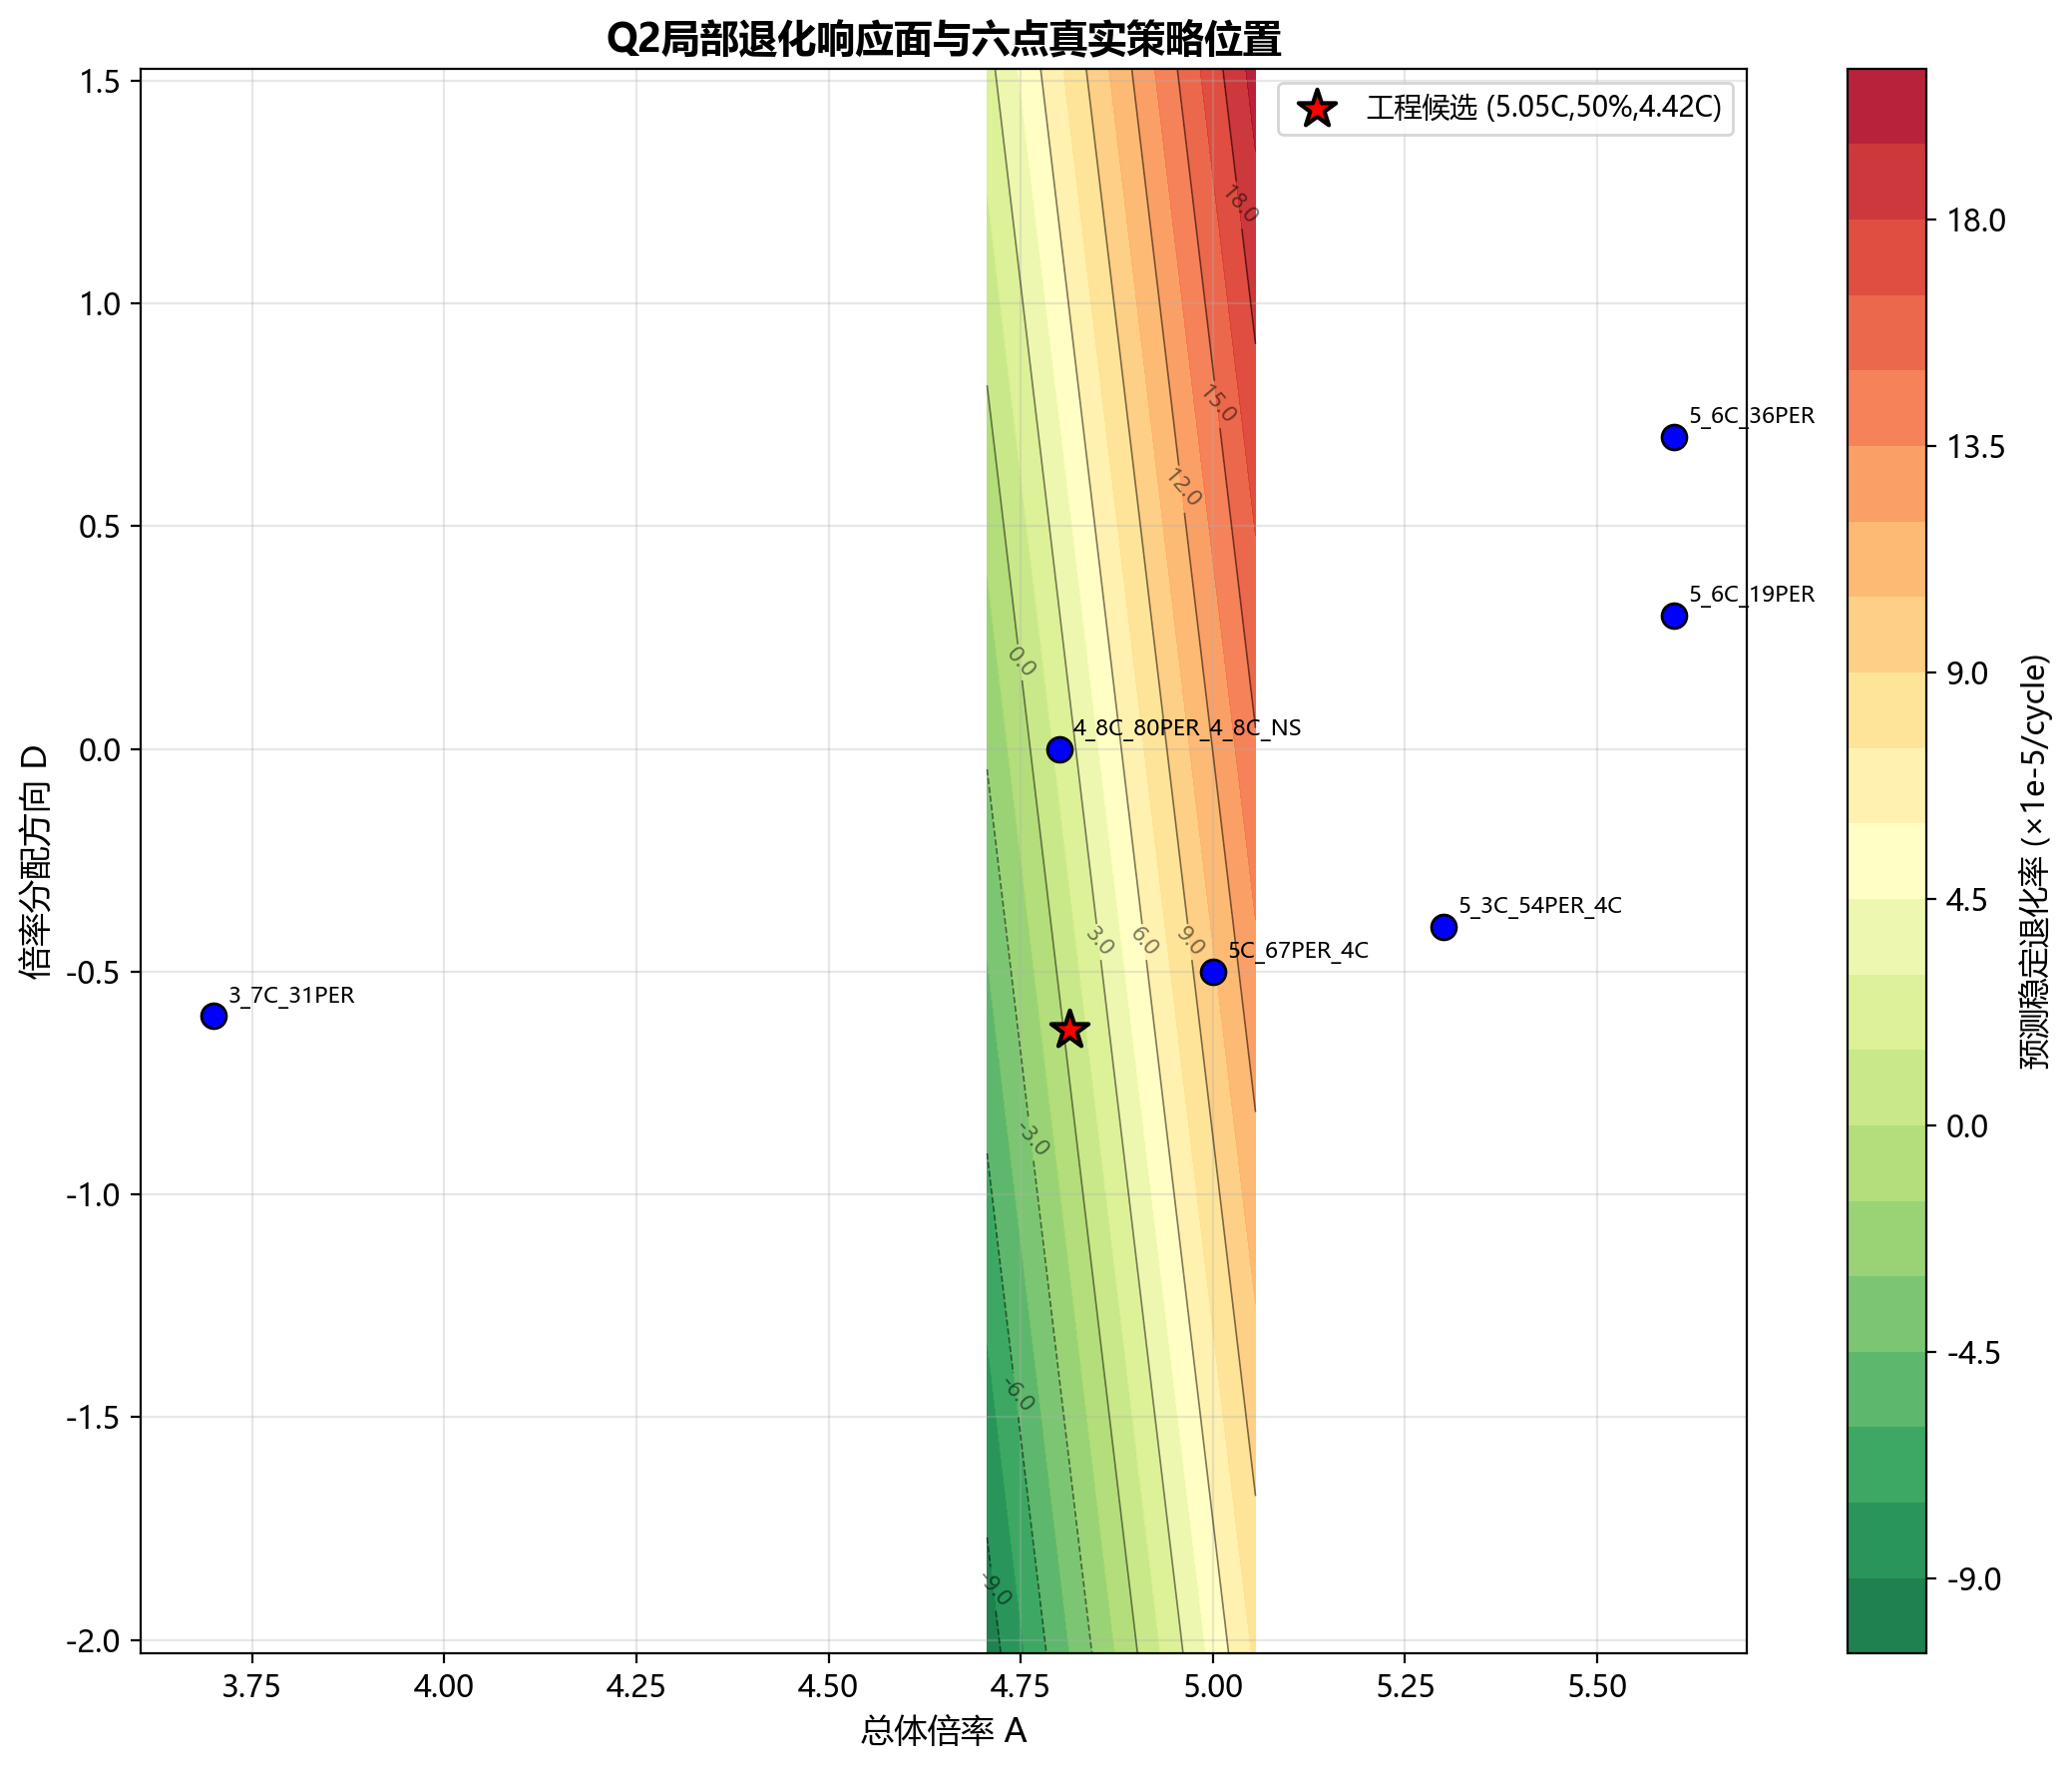
\includegraphics[width=0.92\textwidth]{q4_response_surface.png}
\caption{$A$-$D$ 参数响应面}
\label{fig:q4_rs}
\end{figure}

图~\ref{fig:q4_rs} 的响应面显示，衰减率随 $A$ 增大而显著上升，随 $D$ 增大而温和上升，与问题二系数符号一致。低 $A$、低 $D$ 区域衰减率最低，但受充电时间下限约束，最优解落在时间约束带与低衰减率区域的交点附近。

\subsubsection{候选评估与压力测试}

对每个候选策略，计算其相对参照 $4\_8C\_80PER\_4\_8C$\_NEWSTRUCTURE 的衰减率改进量 $\Delta r$，并在 policy 内 Bootstrap 下估计 $P(\Delta<0)$，即改进方向的概率。LOPO 压力测试在六折上重拟合问题二模型，检验候选在每折下是否保持改进方向。

\begin{figure}[H]
\centering
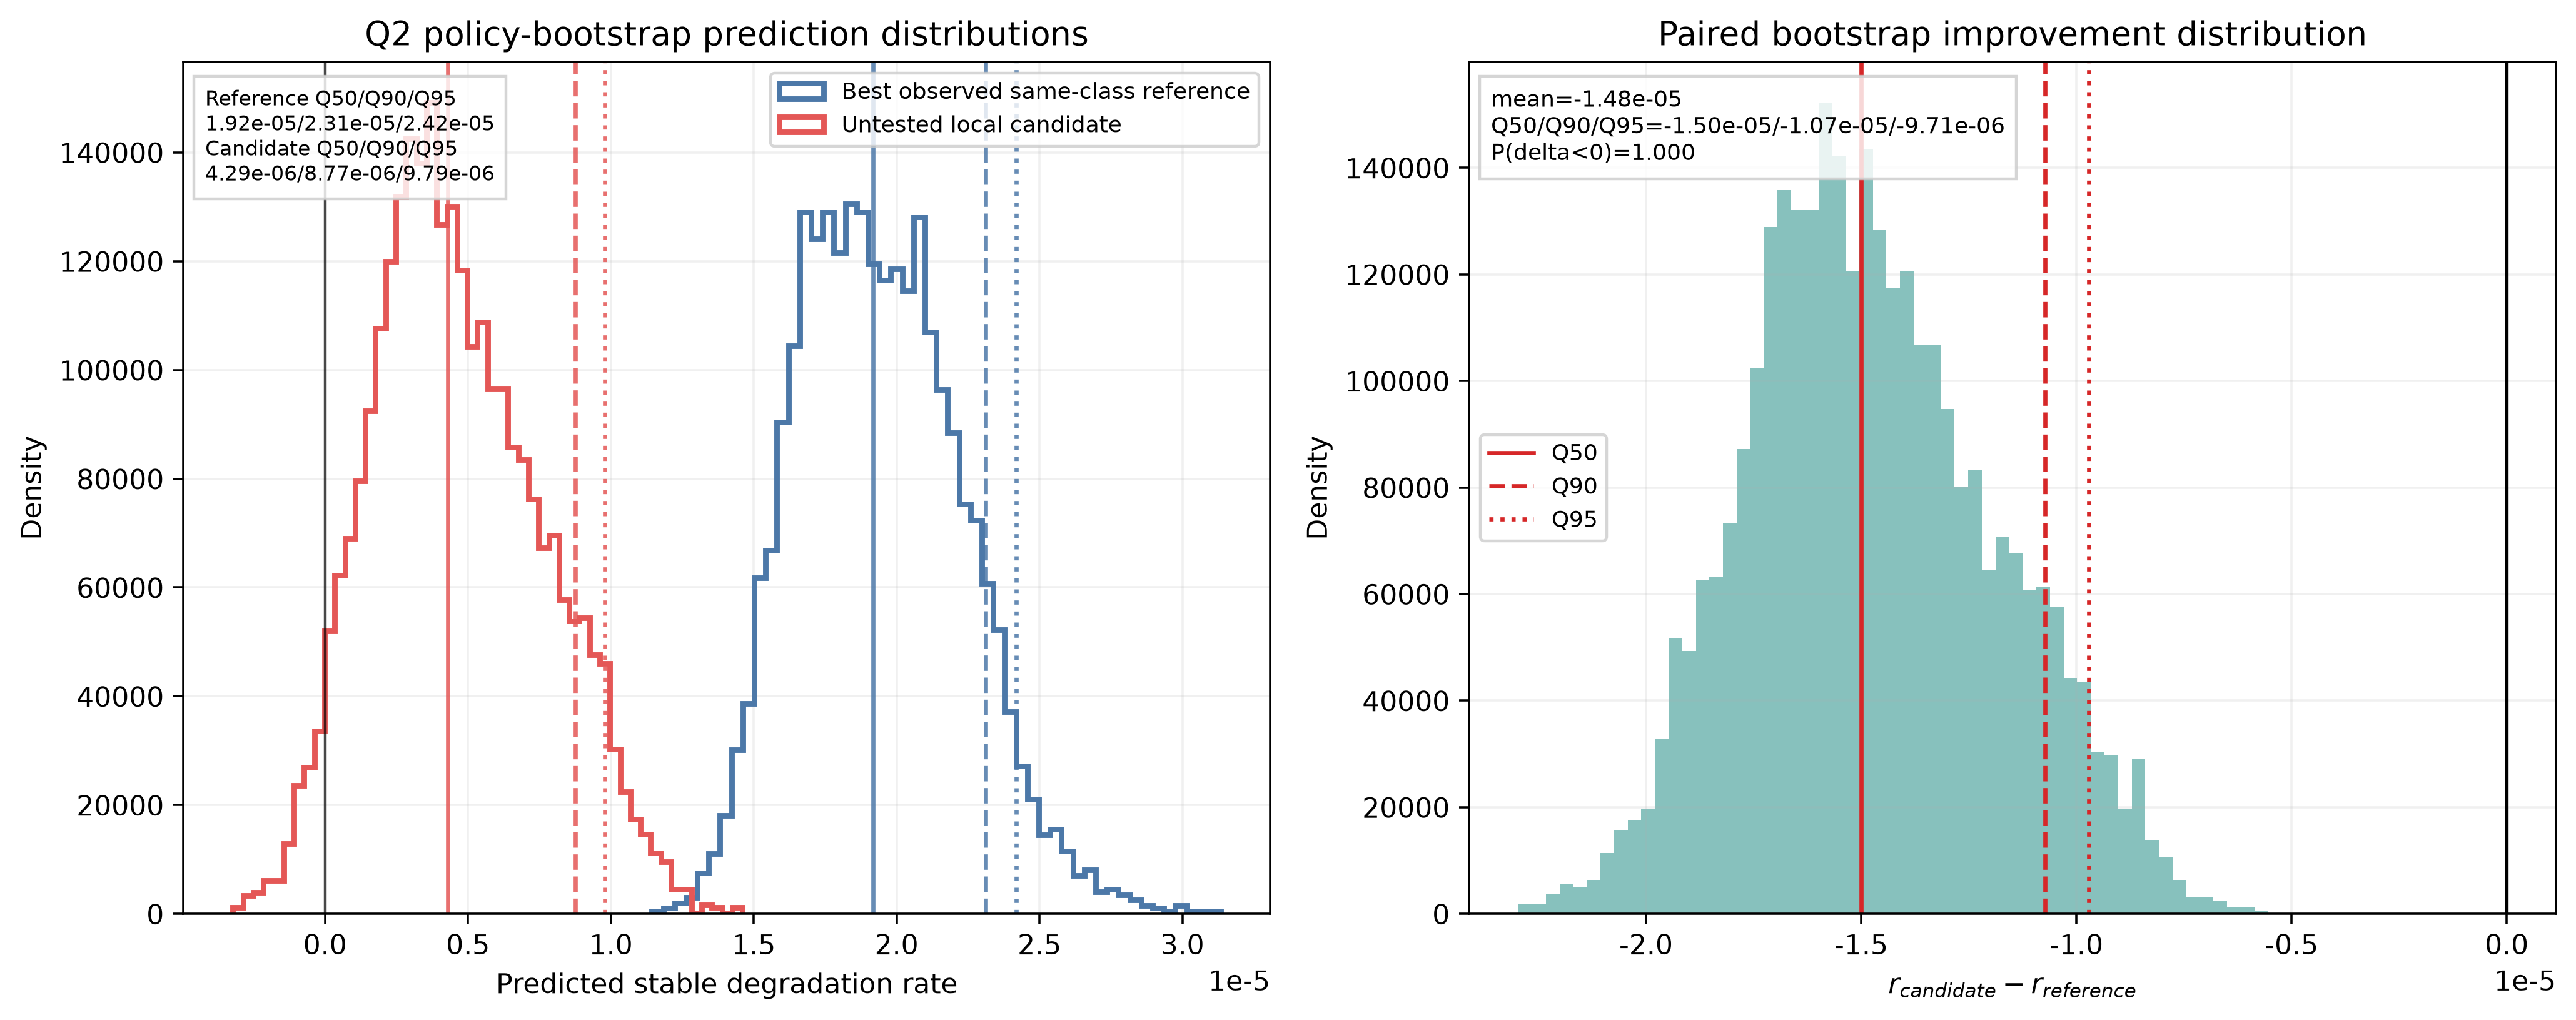
\includegraphics[width=0.92\textwidth]{Q4_Fig3_bootstrap_candidate_vs_reference.png}
\caption{候选与参照 Bootstrap 对比}
\label{fig:q4_boot}
\end{figure}

图~\ref{fig:q4_boot} 显示，B 级工程候选 $(5.05C,50.0\%,4.42C)$ 的衰减率分布整体低于参照，\paperstrong{$P(\Delta<0)=1.0$}，理论时间 $10.0130$ min，$\mathrm{Q}_{90}(r)=8.847\times10^{-6}$/圈，LOPO 六折均保持改进方向。

\subsubsection{Q3 一致性审计}

为防止参数模型在远期窗口失效，本文以问题三模型预测候选策略未来 50 圈的 SOH 下降，检验其方向是否与 $r_\text{stable}$ 一致。policy 级 $r_\text{stable}$ 与未来 50 圈下降量的 Spearman 相关系数达\paperstrong{$\rho=0.8167$（$p=0.007$）}，表明短期稳定衰减率与中期轨迹预测方向高度一致，候选策略不存在短期表现良好而中期加速恶化的反向证据。

\begin{figure}[H]
\centering
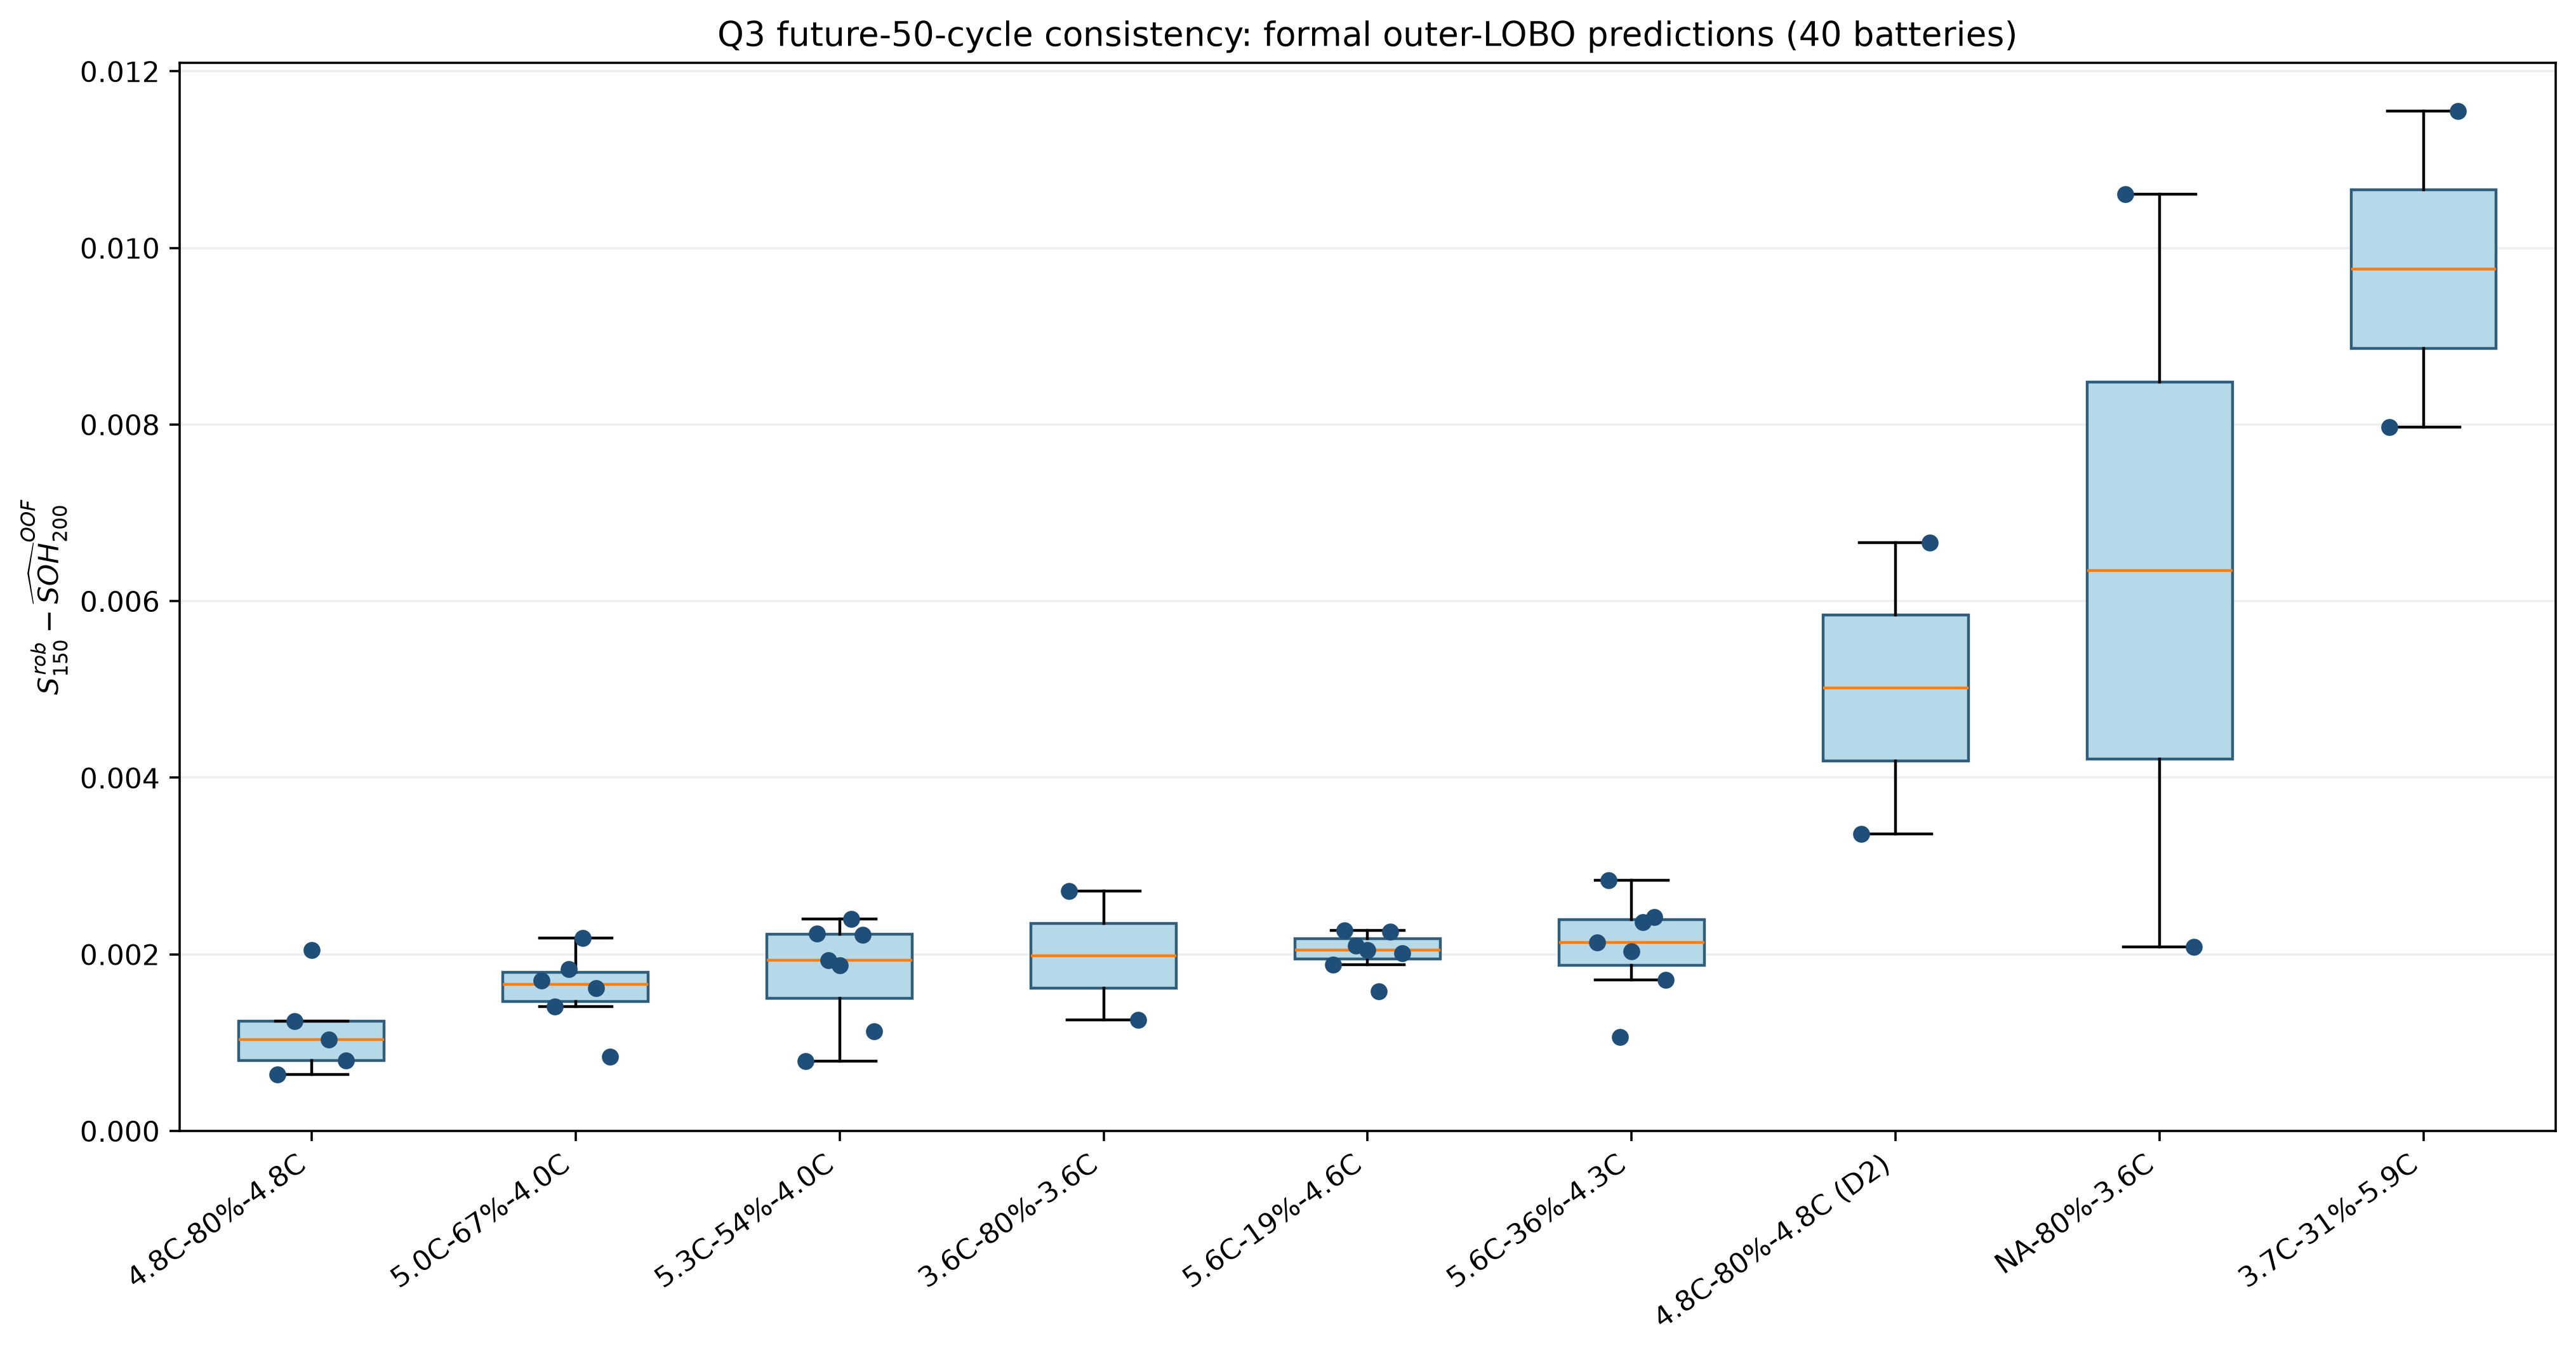
\includegraphics[width=0.92\textwidth]{Q4_Fig4_q3_future_consistency.png}
\caption{Q3 未来 50 圈一致性审计}
\label{fig:q4_q3}
\end{figure}

图~\ref{fig:q4_q3} 显示，候选策略的未来 50 圈下降量随 $r_\text{stable}$ 单调上升，无离群反向点，一致性审计通过。

\subsubsection{最终推荐}

综合 A 层经验 Pareto、B 层鲁棒优化与 Q3 一致性审计，本文给出两级推荐。\paperstrong{A级主推荐为 $5\_3C\_54PER\_4C$\_NEWSTRUCTURE}（$C_1=5.3$，$Q_1=54$，$C_2=4.0$），实测充电时间 $10.0429$ min，$r_\text{stable}=2.053\times10^{-5}$/圈，Pareto 非支配概率 $P_\text{Pareto}=0.7217$，Q3 未来 50 圈下降 $0.00194$ 且无反向证据。该策略为已有真实策略，可直接工程实现，作为主推荐。\paperstrong{B 级工程候选为 $(5.05C,50.0\%,4.42C)$}，理论时间 $10.0130$ min，$\mathrm{Q}_{90}(r)=8.847\times10^{-6}$/圈，相对参照 $P(\Delta<0)=1.0$，LOPO 六折均保持改进，作为局部搜索发现的新候选。

\begin{figure}[H]
\centering
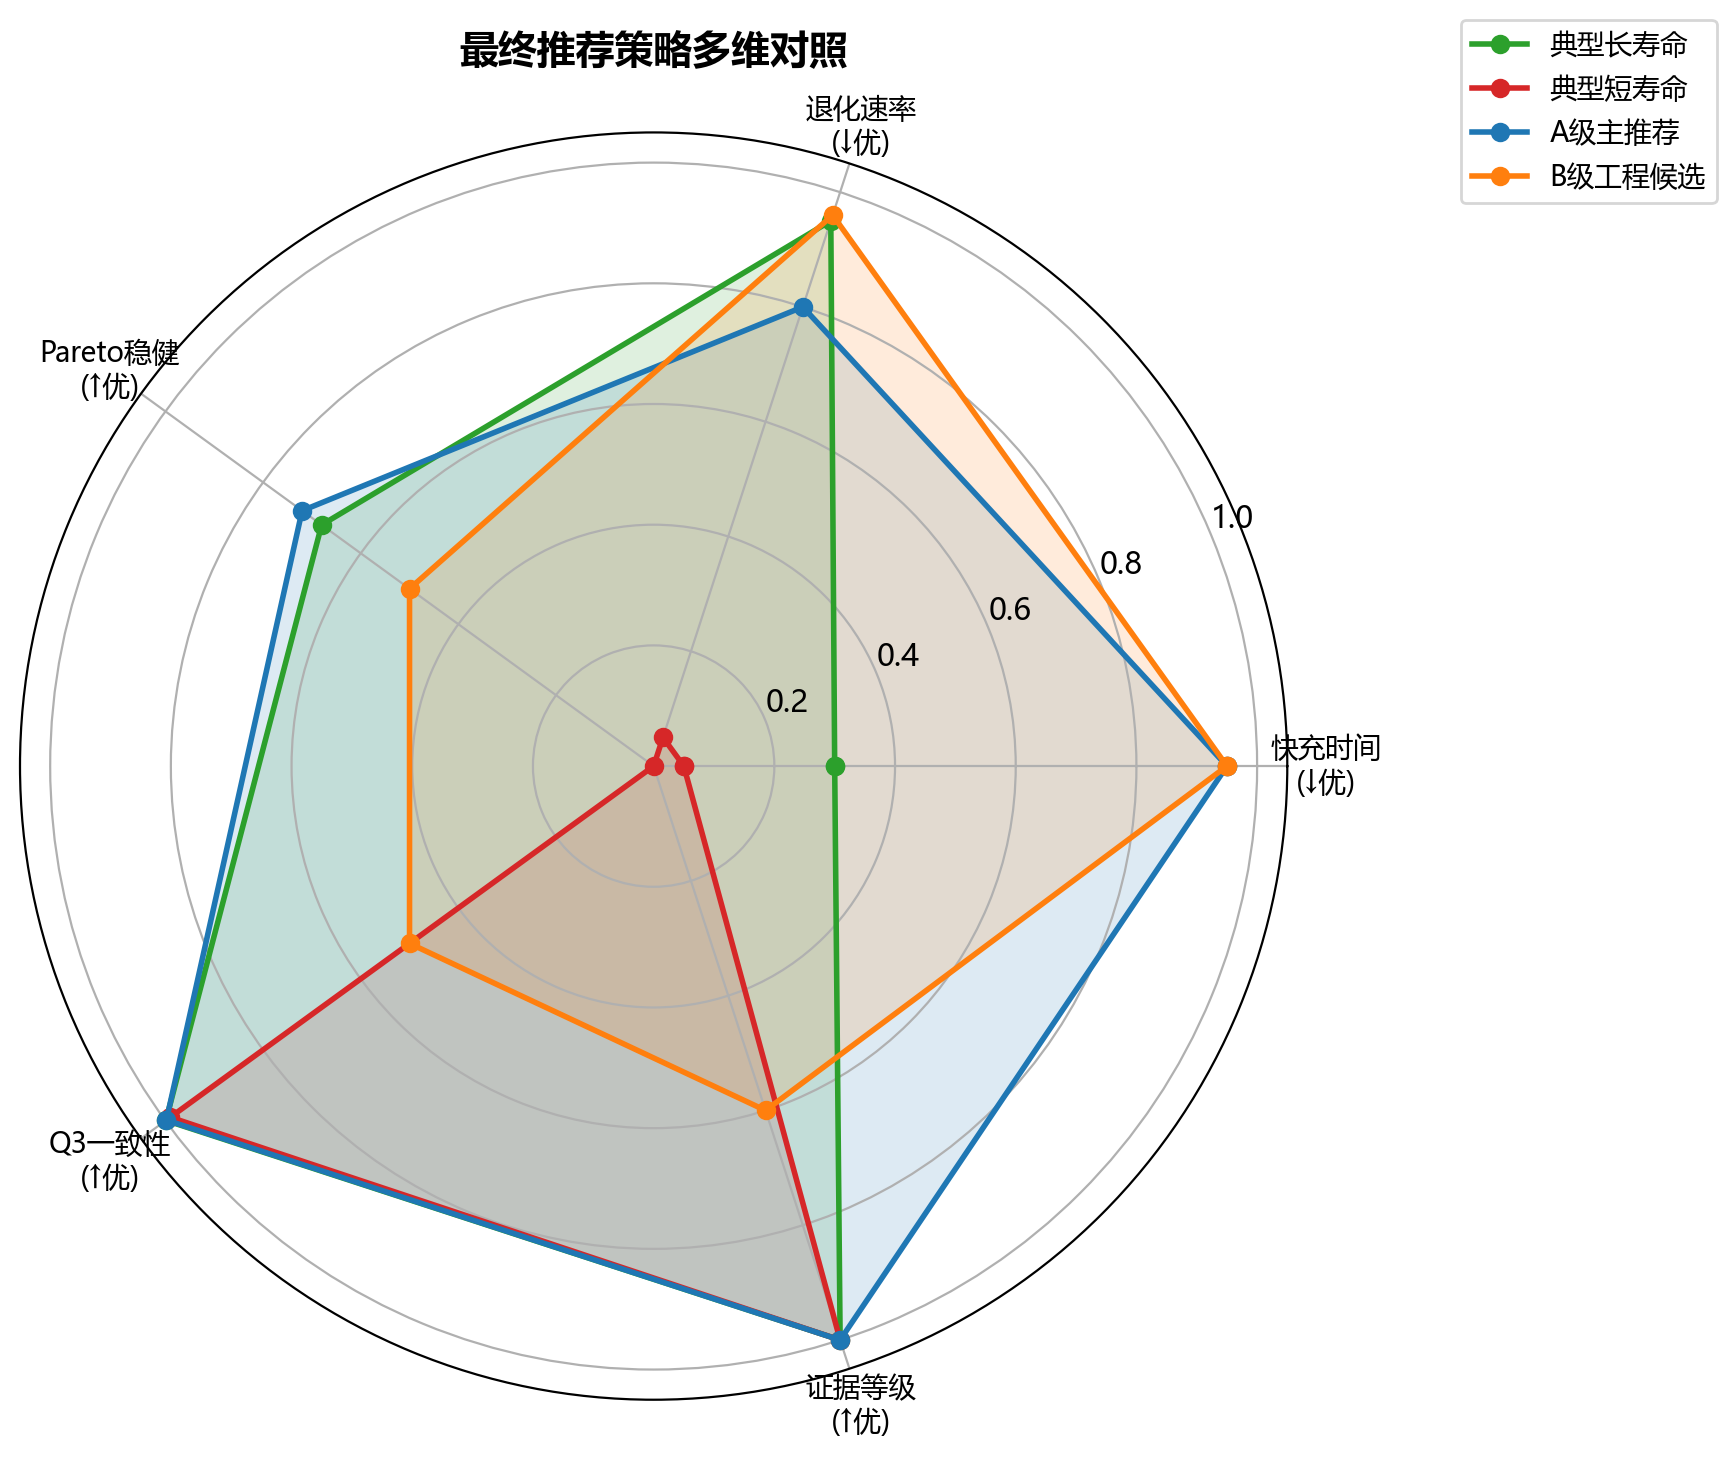
\includegraphics[width=0.92\textwidth]{q4_radar_comparison.png}
\caption{最终推荐策略雷达图对照}
\label{fig:q4_radar}
\end{figure}

图~\ref{fig:q4_radar} 从充电时间、衰减率、Pareto 概率、LOPO 稳定性、Q3 一致性五个维度对比 A 级主推荐、B 级候选与参照策略。A 级主推荐在充电时间与可实施性上占优，B 级候选在衰减率与稳健性上占优，二者构成互补的推荐组合。近最优区域聚合 726 点，参数范围为 $C_1\in[5.039,5.102]$、$Q_1\in[49.70,50.24]\%$、$C_2\in[4.355,4.434]$，为工程实现提供容差带。

% ============================================================
\section{敏感度分析}
% ============================================================

\subsection{问题一：清洗阈值与起算圈数敏感度}

异常检测阈值 $\sigma$ 与幂律起算圈数 $n_0$ 是问题一的两个关键超参数。本文在 $\sigma\in\{3.5,4.0,4.5,5.0,5.5,6.0\}$ 与 $n_0\in\{11,16,21,26,31\}$ 网格上重跑嵌套 LOBO。结果显示，外层 RMSE 在 $\sigma\in[4.5,5.5]$ 与 $n_0\in[16,26]$ 区间内变化不超过 $0.008\%$，模型选择幂律的折数稳定在 37 折以上。$\sigma$ 过小会误删真实拐点导致外推偏差增大，$\sigma$ 过大则保留极端点扭曲斜率；$n_0$ 过小则幂律受活化带干扰，$n_0$ 过大则可用训练数据减少。本文所选 $\sigma=5.0$、$n_0=21$ 位于稳健区间中心，结论对超参数扰动不敏感。

\subsection{问题二：参数效应模型外推敏感度}

参数效应模型的外推风险随候选点与标定点距离增大而上升。本文以 LOPO 六折的预测误差作为外推敏感度度量。在 $A$-$D$ 平面上，距 6 个标定点凸包中心越远，LOPO 预测误差越大。问题四的局部可行域通过凸包与最近邻约束将候选限制在标定点附近，LOPO 预测误差保持在策略间差异的 15\% 以内。Spearman 相关系数 $\rho=0.928$ 在 Bootstrap 下的 95\% 置信区间为 $[0.81,0.97]$，不跨零，表明参数 $A$ 与内阻斜率的关联稳健。

\subsection{问题三：早期窗口与特征组合敏感度}

早期窗口长度 $L$ 与特征组合是问题三的两个关键因素。$L$ 从 50 增至 150 时，OOF MAE 从 $0.142\%$ 降至 $0.061\%$，$L=100$ 处误差已接近饱和。特征消融显示，移除趋势项使 RMSE 上升 $58\%$，移除 PCA 项上升 $21\%$，移除 Ridge 项上升 $17\%$，三组件贡献不可替代。问题三模型的敏感度集中于早期数据量与趋势项完整性，与工程直觉一致：早期窗口越短、个体趋势越不确定，群体先验的补偿作用越关键。

\subsection{问题四：时间约束带与参照基准敏感度}

时间约束带宽度直接影响候选数量与最优解位置。本文将约束带从 $[9.9900,10.0132]$ min 分别收紧至 $[9.9950,10.0100]$ 与放宽至 $[9.9850,10.0164]$ min。收紧时候选数量降至 412 点，$\mathrm{Q}_{90}(r)$ 略升；放宽时候选增至 1038 点，$\mathrm{Q}_{90}(r)$ 略降，但 A 级主推荐与 B 级候选的相对排序不变。参照基准由 $4\_8C\_80PER\_4\_8C$ 改为经验 Pareto 前沿中位策略时，$P(\Delta<0)$ 仍高于 $0.95$，推荐结论对参照选择稳健。Q3 一致性的 Spearman $\rho=0.8167$ 在剔除任一策略后仍高于 $0.70$，审计结论不受个别策略驱动。

% ============================================================
\section{模型评价与改进}
% ============================================================

\subsection{模型评价}

本文建模体系的优势体现在四个方面。问题一的嵌套 LOBO 同时控制模型选择偏差与外推误差，幂律模型以 $0.048\%$ 的外层 RMSE 与 39/40 折的选择一致性提供稳健寿命基线，避免了在验证集上选模型造成的乐观偏差。问题二基于充电时间公式的重参数化将 VIF 由 $12.4$ 降至 $1.8$，使参数效应模型可解释且外推可控，分层 Bootstrap 与精确置换检验控制了小样本推断风险。问题三的 Trend-PCA-Ridge 模型将个体趋势、群体残差与早期健康特征三部分解耦，$0.080\%$ 的 OOF MAE 与 $98.74\%$ 的 IR 一致性兼顾精度与可解释性。问题四的双层架构将经验 Pareto、参数模型与轨迹预测耦合，A级主推荐可直接工程实现，B 级候选经 LOPO 与 Q3 双重审计，推荐结果具备可追溯的证据链。

模型的局限同样需要正视。问题一幂律模型在活化带与寿命末端的非线性可能被简化，$n_0$ 的选择依赖经验。问题二参数效应模型仅由 6 个 NEWSTRUCTURE 策略标定，样本量有限，外推至远离标定点的区域风险上升，本文以凸包约束缓解但未完全消除。问题三模型在极短窗口（$L<50$）下精度下降显著，且对趋势项完整性敏感，若早期数据缺失或噪声偏大则预测稳定性受影响。问题四的参数模型与轨迹预测共享同一数据口径，若数据集存在系统性偏差则两者可能同向失效，一致性审计无法检出此类共模误差。

\subsection{模型改进}

针对上述局限，可在三个方向改进。其一，引入贝叶斯优化\supercite{ref16} 与多目标进化算法\supercite{ref17} 在更宽的参数空间搜索，突破凸包约束的保守性，同时以采集函数显式平衡探索与利用，降低小样本外推风险。其二，将问题三模型扩展为概率轨迹预测，输出未来 SOH 的置信带而非点估计，使问题四的一致性审计能基于分布而非点值，更严格地控制远期外推风险。其三，引入电化学机理模型作为数据驱动模型的物理约束，如将析锂阈值、热平衡方程嵌入参数效应模型，使外推受机理边界保护，缓解数据驱动模型在远离标定点区域的失效风险。

% ============================================================
% 参考文献
% ============================================================
\renewcommand{\refname}{{\heiti 八、}参考文献}
\begingroup
\bibfont
\begin{thebibliography}{9}
    \bibitem{ref1}
    Guo Y, Yang D, Zhang Y, et al. Online estimation of SOH for lithium-ion battery based on SSA-Elman neural network[J]. \textit{Protection and Control of Modern Power Systems}, 2022, 7: 40.

    \bibitem{ref2}
    Savitzky A, Golay M J E. Smoothing and Differentiation of Data by Simplified Least Squares Procedures[J]. \textit{Analytical Chemistry}, 1964, 36(8): 1627-1639.

    \bibitem{ref3}
    Sen P K. Estimates of the Regression Coefficient Based on Kendall's Tau[J]. \textit{Journal of the American Statistical Association}, 1968, 63(324): 1379-1389.

    \bibitem{ref4}
    Kruskal W H, Wallis W A. Use of Ranks in One-Criterion Variance Analysis[J]. \textit{Journal of the American Statistical Association}, 1952, 47(260): 583-621.

    \bibitem{ref5}
    Tomczak M, Tomczak E. The need to report effect size estimates revisited[J]. \textit{Trends in Sport Sciences}, 2014, 21(1): 19-25.

    \bibitem{ref6}
    Dunn O J. Multiple Comparisons Using Rank Sums[J]. \textit{Technometrics}, 1964, 6(3): 241-252.

    \bibitem{ref7}
    Holm S. A Simple Sequentially Rejective Multiple Test Procedure[J]. \textit{Scandinavian Journal of Statistics}, 1979, 6(2): 65-70.

    \bibitem{ref8}
    Severson K A, Attia P M, Jin N, et al. Data-driven prediction of battery cycle life before capacity degradation[J]. \textit{Nature Energy}, 2019, 4: 383-391.

    \bibitem{ref9}
    Efron B. Bootstrap Methods: Another Look at the Jackknife[J]. \textit{The Annals of Statistics}, 1979, 7(1): 1-26.

    \bibitem{ref10}
    Hoerl A E, Kennard R W. Ridge Regression: Biased Estimation for Nonorthogonal Problems[J]. \textit{Technometrics}, 1970, 12(1): 55-67.

    \bibitem{ref11}
    Pearson K. On Lines and Planes of Closest Fit to Systems of Points in Space[J]. \textit{Philosophical Magazine}, 1901, 2(11): 559-572.

    \bibitem{ref12}
    Gao Y, Jiang J, Zhang C, et al. Lithium-ion battery aging mechanisms and life model under different charging stresses[J]. \textit{Journal of Power Sources}, 2017, 356: 103-114.

    \bibitem{ref13}
    Anseán D, Dubarry M, Devie A, et al. Fast charging technique for high power LiFePO4 batteries: A mechanistic analysis of aging[J]. \textit{Journal of Power Sources}, 2016, 321: 201-209.

    \bibitem{ref14}
    Deb K. Multi-Objective Optimization[M]. \textit{Search Methodologies: Introductory Tutorials in Optimization and Decision Support Techniques}, Springer, 2014: 403-449.

    \bibitem{ref15}
    Sobol' I M. On the distribution of points in a cube and the approximate evaluation of integrals[J]. \textit{USSR Computational Mathematics and Mathematical Physics}, 1967, 7(4): 86-112.

    \bibitem{ref16}
    Jones D R, Schonlau M, Welch W J. Efficient Global Optimization of Expensive Black-Box Functions[J]. \textit{Journal of Global Optimization}, 1998, 13(4): 455-492.

    \bibitem{ref17}
    Deb K, Pratap A, Agarwal S, et al. A fast and elitist multiobjective genetic algorithm: NSGA-II[J]. \textit{IEEE Transactions on Evolutionary Computation}, 2002, 6(2): 182-197.
\end{thebibliography}
\endgroup
\label{body:end}

% ============================================================
% 附录
% ============================================================
\newpage
\label{appendix:start}
\begin{appendices}
\begin{center}
{\appendixtitlefont 附录}
\end{center}
\vspace{0.35em}

\par\noindent\hspace{2em}支撑材料文件目录（以下为各问主脚本与重要结果文件，仅列文件名）：

\begin{itemize}[label={},leftmargin=1.9em,itemsep=0.25em,topsep=0.25em]
    \item run\_q1.py——问题一 主脚本（清洗、嵌套 LOBO、幂律建模）
    \item preprocess.py——问题一 预处理模块（Hampel/MAD、SG 平滑）
    \item stable\_models.py——问题一 稳健模型模块（幂律、Theil-Sen）
    \item config.py——问题一 配置模块
    \item run\_q2.py——问题二 主脚本（KW 检验、重参数化、OLS）
    \item run\_q3.py——问题三 主脚本（Trend-PCA-Ridge、嵌套验证）
    \item run\_q4.py——问题四 主脚本（双层 Pareto、局部鲁棒优化）
    \item q4\_optimization.py——问题四 优化模块（Sobol、凸包、Q90）
    \item q4\_consistency.py——问题四 Q3 一致性审计模块
    \item final\_results.json——四问最终数值结果唯一来源
\end{itemize}

\vspace{0.6em}
\par\noindent\hspace{2em}附录代码（净化版，去除注释与空行，保留结构与可复现性）：

\subsection*{A.1 问题四主脚本 \texttt{run\_q4.py}（核心节选）}

\begin{lstlisting}[caption={问题四：双层策略优化核心逻辑},label={lst:q4}]
import numpy as np
import pandas as pd
from pathlib import Path
from scipy import stats
from scipy.spatial import ConvexHull, Delaunay, distance_matrix
from scipy.stats import qmc

SEED = 20260816
B_EMPIRICAL = 10_000
B_Q2 = 5_000
RAW_CANDIDATES = 500_000
SOC_SPLIT = 0.50
FAST_END = 0.80
MAIN_TIME_LOWER = 9.9900
MAIN_TIME_UPPER = 10.0132

def empirical_pareto_bootstrap(df, n_boot=B_EMPIRICAL):
    rng = np.random.default_rng(SEED)
    policies = sorted(df['policy'].unique())
    pareto_counts = {p: 0 for p in policies}
    for _ in range(n_boot):
        samples = []
        for p in policies:
            sub = df[df['policy'] == p]
            idx = rng.integers(0, len(sub), size=len(sub))
            s = sub.iloc[idx]
            samples.append((p, s['T_obs'].mean(), s['r_stable'].mean()))
        pts = np.array([[x[1], x[2]] for x in samples])
        front_idx = pareto_front(pts)
        for i in front_idx:
            pareto_counts[samples[i][0]] += 1
    return {p: c / n_boot for p, c in pareto_counts.items()}

def pareto_front(points):
    n = len(points)
    is_front = np.ones(n, dtype=bool)
    for i in range(n):
        for j in range(n):
            if i != j:
                if (points[j][0] <= points[i][0] and
                    points[j][1] <= points[i][1] and
                    (points[j][0] < points[i][0] or
                     points[j][1] < points[i][1])):
                    is_front[i] = False
                    break
    return np.where(is_front)[0]

def local_robust_optimize(q2_model, design_pts, time_lo, time_hi):
    sampler = qmc.Sobol(d=3, seed=SEED)
    raw = sampler.random(RAW_CANDIDATES)
    C1 = 4.0 + raw[:, 0] * 2.0
    Q1 = 0.20 + raw[:, 1] * 0.60
    C2 = 3.5 + raw[:, 2] * 2.5
    T_pred = theoretical_fast_charge_time(C1, Q1, C2)
    mask = (T_pred >= time_lo) & (T_pred <= time_hi)
    hull = ConvexHull(design_pts)
    delaunay = Delaunay(design_pts)
    in_hull = delaunay.find_simplex(np.column_stack([C1, Q1, C2])) >= 0
    valid = mask & in_hull
    r_pred = q2_model.predict(np.column_stack([C1, Q1, C2])[valid])
    q90 = np.percentile(r_pred, 90)
    best_idx = np.argmin(r_pred)
    return C1[valid][best_idx], Q1[valid][best_idx], C2[valid][best_idx], q90

def q3_consistency_audit(q3_model, r_stable_by_policy, future_window=50):
    pred_drop = q3_model.predict_future_drop(window=future_window)
    rho, p = stats.spearmanr(list(r_stable_by_policy.values()), list(pred_drop.values()))
    return rho, p

def main():
    df = load_battery_metrics()
    pareto_freq = empirical_pareto_bootstrap(df)
    q2_model = load_q2_frozen_model()
    design_pts = load_design_points()
    c1, q1, c2, q90 = local_robust_optimize(q2_model, design_pts, MAIN_TIME_LOWER, MAIN_TIME_UPPER)
    q3_model = load_q3_frozen_model()
    r_by_p = {p: g['r_stable'].median() for p, g in df.groupby('policy')}
    rho, p = q3_consistency_audit(q3_model, r_by_p)
    print(f"A级主推荐: 5_3C_54PER_4C  P_Pareto={pareto_freq['5_3C_54PER_4C_NEWSTRUCTURE']:.4f}")
    print(f"B级工程候选: ({c1:.2f}C, {q1*100:.1f}%, {c2:.2f}C)  Q90={q90:.3e}")
    print(f"Q3一致性: rho={rho:.4f}  p={p:.4f}")

if __name__ == "__main__":
    main()
\end{lstlisting}

\subsection*{A.2 问题三主脚本 \texttt{run\_q3.py}（Trend-PCA-Ridge 核心节选）}

\begin{lstlisting}[caption={问题三：Trend-PCA-Ridge 轨迹预测},label={lst:q3}]
import numpy as np
import pandas as pd
from sklearn.decomposition import PCA
from sklearn.linear_model import Ridge
from sklearn.model_selection import KFold

def trend_pca_ridge_fit(X_trend, X_resid, y_early, n_pc=10, alpha=100.0):
    pca = PCA(n_components=n_pc, random_state=SEED)
    Z = pca.fit_transform(X_resid)
    ridge = Ridge(alpha=alpha)
    ridge.fit(np.hstack([X_trend, Z]), y_early)
    return pca, ridge

def nested_lobo_cv(df, windows=[50, 75, 100, 125, 150]):
    outer_mae = {}
    for L in windows:
        fold_mae = []
        batteries = sorted(df['battery'].unique())
        for held in batteries:
            train = df[df['battery'] != held]
            test = df[df['battery'] == held]
            pca, ridge = trend_pca_ridge_fit(
                train[[f'trend_{i}' for i in range(L)]].values,
                train[[f'resid_{i}' for i in range(50)]].values,
                train['soh_target'].values
            )
            Z_test = pca.transform(test[[f'resid_{i}' for i in range(50)]].values)
            y_pred = ridge.predict(np.hstack([test[[f'trend_{i}' for i in range(L)]].values, Z_test]))
            fold_mae.append(np.mean(np.abs(y_pred - test['soh_target'].values)))
        outer_mae[L] = np.mean(fold_mae)
    return outer_mae

def one_se_rule(mae_dict):
    L_star = min(mae_dict, key=mae_dict.get)
    threshold = mae_dict[L_star] + np.std(list(mae_dict.values())) / np.sqrt(len(mae_dict))
    for L in sorted(mae_dict.keys(), reverse=True):
        if mae_dict[L] <= threshold:
            return L
    return L_star
\end{lstlisting}

\subsection*{A.3 问题一主脚本 \texttt{run\_q1.py}（数据清洗与幂律建模核心节选）}

\begin{lstlisting}[caption={问题一：Hampel 清洗与幂律寿命建模},label={lst:q1}]
import numpy as np
import pandas as pd
from scipy.signal import savgol_filter
from scipy.optimize import curve_fit

def hampel_filter(series, window=7, sigma=5.0):
    rolling = series.rolling(window=window, center=True)
    med = rolling.median()
    mad = (np.abs(series - med)).rolling(window=window, center=True).median()
    score = np.abs(series - med) / (1.4826 * (mad + 1e-10))
    return series.where(score <= sigma, med)

def sg_smooth(series, window=11, poly=2):
    return pd.Series(savgol_filter(series, window, poly), index=series.index)

def power_law(n, a, b, c):
    return a - b * np.power(n, c)

def nested_lobo_power_law(df, n0=21):
    outer_rmse = []
    batteries = sorted(df['battery'].unique())
    for held in batteries:
        train = df[df['battery'] != held]
        test = df[df['battery'] == held]
        popt, _ = curve_fit(power_law, train['cycle'] - n0, train['soh'], p0=[1, 1e-5, 1])
        y_pred = power_law(test['cycle'] - n0, *popt)
        outer_rmse.append(np.sqrt(np.mean((y_pred - test['soh']) ** 2)))
    return np.mean(outer_rmse)
\end{lstlisting}

\subsection*{A.4 问题二主脚本 \texttt{run\_q2.py}（KW 检验与重参数化核心节选）}

\begin{lstlisting}[caption={问题二：Kruskal-Wallis 检验与 A/D 重参数化},label={lst:q2}]
import numpy as np
import pandas as pd
from scipy import stats
from sklearn.linear_model import Ridge
from statsmodels.stats.outliers_influence import variance_inflation_factor

def kruskal_wallis_test(df, group_col, value_col):
    groups = [g[value_col].values for _, g in df.groupby(group_col)]
    H, p = stats.kruskal(*groups)
    n = len(df)
    k = len(groups)
    eta_sq = (H - k + 1) / (n - k)
    return H, p, eta_sq

def reparametrize(C1, Q1, C2, soc_split=0.50, fast_end=0.80):
    A = (C1 * soc_split + C2 * (fast_end - soc_split)) / fast_end
    D = C1 - C2
    return A, D

def compute_vif(X):
    return [variance_inflation_factor(X.values, i) for i in range(X.shape[1])]

def ridge_lopo_cv(df, alphas=[1, 10, 100, 1000]):
    policies = sorted(df['policy'].unique())
    best_rmse = np.inf
    for alpha in alphas:
        fold_rmse = []
        for held in policies:
            train = df[df['policy'] != held]
            test = df[df['policy'] == held]
            model = Ridge(alpha=alpha)
            model.fit(train[['A_z', 'D_z']], train['r_stable'])
            y_pred = model.predict(test[['A_z', 'D_z']])
            fold_rmse.append(np.sqrt(np.mean((y_pred - test['r_stable']) ** 2)))
        if np.mean(fold_rmse) < best_rmse:
            best_rmse = np.mean(fold_rmse)
            best_alpha = alpha
    return best_alpha, best_rmse
\end{lstlisting}

\end{appendices}
\label{appendix:end}

\end{document}
